%\documentclass{sig-alternate-05-2015}
\documentclass[acmlarge, ,11pt]{acmart}
%\citestyle{acmauthoryear}
%\usepackage{booktabs} % For formal tables
\usepackage[ruled]{algorithm2e} % For algorithms
\usepackage{subfigure}
\usepackage{marvosym}
\usepackage{mathtools}
\usepackage{caption}
\usepackage{algpseudocode}
%\usepackage{algorithm}
\usepackage{graphicx}
\usepackage[T1]{fontenc}
\usepackage{tikz}
\usepackage{listings}
\usepackage{amsmath,bm,times,amssymb}
\usepackage{textcomp}
 %\newtheorem {theorem} {Theorem}
 %\newtheorem{corollary} {corollary} [theorem] 
\DeclarePairedDelimiterX\Set[2]{\lbrace}{\rbrace}%
{ #1 \,\delimsize|\,\mathopen{} #2 }
\newsavebox{\ieeealgbox}
\newenvironment{boxedalgorithmic}
  {\begin{lrbox}{\ieeealgbox}
   \begin{minipage}{\dimexpr\columnwidth-2\fboxsep-2\fboxrule}
   \begin{algorithmic}}
  {\end{algorithmic}
   \end{minipage}
   \end{lrbox}\noindent\fbox{\usebox{\ieeealgbox}}}
\lstset{ %
language=Java,                % choose the language of the code
%basicstyle=\scriptsize,       % the size of the fonts that are used for the code
%basicstyle=\sffamily,
basicstyle={\footnotesize \sffamily},
%numbers=left,                   % where to put the line-numbers
%numberstyle=\footnotesize,      % the size of the fonts that are used for the line-numbers
%stepnumber=1,                   % the step between two line-numbers. If it's 1 each line
                                % will be numbered
%numbersep=2pt,                  % how far the line-numbers are from the code
backgroundcolor=\color{white},  % choose the background color. You must add \usepackage{color}
showspaces=false,               % show spaces adding particular underscores
showstringspaces=false,         % underline spaces within strings
showtabs=false,                 % show tabs within strings adding particular underscores
frame=none,                    % adds a frame around the code
tabsize=2,                      % sets default tabsize to 2 spaces
captionpos=none,                % sets the caption-position to bottom
breaklines=true,                % sets automatic line breaking
breakatwhitespace=false,        % sets if automatic breaks should only happen at whitespace
title=\lstname,                 % show the filename of files included with \lstinputlisting;
                                % also try caption instead of title
escapeinside={\%*}{*)},         % if you want to add a comment within your code
%morekeywords={Definition, Theorem, Fixpoint}            % if you want to add more keywords to the set
}
\begin{document}
\title{A Consistent Understanding of Consistency} 
%\numberofauthors{3} %  in this sample file, there are a *total*
%% of EIGHT authors. SIX appear on the 'first-page' (for formatting
%% reasons) and the remaining two appear in the \additionalauthors section.
%%
\author{Subhajit Sidhanta}
\authornote{The corresponding author}
%\orcid{1234-5678-9012-3456}
\email{ssidhanta@gsd.inesc-id.pt}
\affiliation{%
  \institution{INESC-ID}
%  \department{School of Engineering}
%  \city{Charlottesville}
%  \state{VA}
%  \postcode{22903}
  \country{Portugal}
}
\author{Ricardo Dias}
\email{ricardo.dias@gmail.com}
\affiliation{%
  \institution{SUSE Linux GmbH}
%  \city{Prague}
%  \country{Czech Republic}}
%\author{Tian He}
%\affiliation{%
%  \institution{University of Minnesota}
  \country{Portugal}}
\author{Rodrigo Rodrigues}
\email{rodrigo@gsd.inesc-id.pt}
\affiliation{%
  \institution{INESC-ID/IST (U.\ Lisboa)}
%  \city{Charlottesville}
%  \state{VA}
%  \postcode{22903}
  \country{Portugal}
}
  
%\author{
%% You can go ahead and credit any number of authors here,
%% e.g. one 'row of three' or two rows (consisting of one row of three
%% and a second row of one, two or three).
%%
%% The command \alignauthor (no curly braces needed) should
%% precede each author name, affiliation/snail-mail address and
%% e-mail address. Additionally, tag each line of
%% affiliation/address with \affaddr, and tag the
%% e-mail address with \email.
%%
%% 1st. author
%
%\alignauthor
%Subhajit Sidhanta\\%\titlenote{Dr.~Trovato insisted his name be first.}\\
%       \affaddr{INESC-ID/IST}\\
%       %\affaddr{1932 Wallamaloo Lane}\\
%       %\affaddr{Wallamaloo, New Zealand}\\
%       %\email{ssidhanta@gsd.inesc-id.pt}
%% 2nd. author
%\alignauthor
%Ricardo Dias\\%Tobin\titlenote{The secretary disavows
%%any knowledge of this author's actions.}\\
%       \affaddr{SUSE Linux GmbH}\\
%       %\affaddr{P.O. Box 1212}\\
%       %\affaddr{Dublin, Ohio 43017-6221}\\
%       %\email{ricardo.dias@gmail.com}
%% 3rd. author
%\alignauthor %Lars Th{\o}rv{\"a}ld\titlenote{This author is the
%Rodrigo Rodrigues\\ %one who did all the really hard work.}\\
%       \affaddr{INESC-ID/IST}\\
%       %\affaddr{1 Th{\o}rv{\"a}ld Circle}\\
%       %\affaddr{Hekla, Iceland}\\
%       %\email{rodrigo.miragaia.rodrigues@tecnico.ulisboa.pt}
%%\and  % use '\and' if you need 'another row' of author names
%%% 4th. author
%%\alignauthor Lawrence P. Leipuner\\
%%       \affaddr{Brookhaven Laboratories}\\
%%       \affaddr{Brookhaven National Lab}\\
%%       \affaddr{P.O. Box 5000}\\
%%       \email{lleipuner@researchlabs.org}
%%% 5th. author
%%\alignauthor Sean Fogarty\\
%%       \affaddr{NASA Ames Research Center}\\
%%       \affaddr{Moffett Field}\\
%%       \affaddr{California 94035}\\
%%       \email{fogartys@amesres.org}
%%% 6th. author
%%\alignauthor Charles Palmer\\
%%       \affaddr{Palmer Research Laboratories}\\
%%       \affaddr{8600 Datapoint Drive}\\
%%       \affaddr{San Antonio, Texas 78229}\\
%%       \email{cpalmer@prl.com}
%}
% There's nothing stopping you putting the seventh, eighth, etc.
% author on the opening page (as the 'third row') but we ask,
% for aesthetic reasons that you place these 'additional authors'
% in the \additional authors block, viz.
%\additionalauthors{Additional authors: John Smith (The Th{\o}rv{\"a}ld Group,
%email: {\texttt{jsmith@affiliation.org}}) and Julius P.~Kumquat
%(The Kumquat Consortium, email: {\texttt{jpkumquat@consortium.net}}).}
%\date{30 July 1999}
% Just remember to make sure that the TOTAL number of authors
% is the number that will appear on the first page PLUS the
% number that will appear in the \additionalauthors section.

\maketitle
\begin{abstract}
 We propose a specification language named \emph{ConSpec}, which enables the formalization of
 different consistency semantics that a storage system may provide, using a simple and uniform syntax, which is independent
 of the design and implementation of the target storage system. ConSpec addresses the recent profusion of consistency definitions,
 which are often accompanied by either informal definitions, or definitions that are tied to implementation-level details.
% Furthermore, even in the case of consistency models that have a precise definition associated with them, 
%  Prior to ConSpec, definitions of
%  consistency models were tightly coupled with the specific design and implementation of the target storage system.
%  Each new storage system would redefine a consistency model in terms of its design and implementation. T
%   the absence of a uniform notation for describing different models 
%   makes it difficult to compare different proposals.
%  Existing
%  definitions of consistency models and isolation levels either use textual descriptions or graphical representation of
%  proscribed anomalies and allowed dependencies between operations, making
%   automated verification even more difficult. To the best of our knowledge, this is the first work that expresses both
%   consistency and isolation levels in terms of ConSpec, a language that
To enable a simple and uniform description of various existing proposals, ConSpec builds on recent proposals that view weak consistency
definitions as partial orderings between operations forming a visibility graph, which reduces the consistency definition to a set of
restrictions on those partial orders, described using Linear Temporal Logic (LTL). We use ConSpec to revisit several existing models in light 
of a common way to define and compare them. Furthermore, the use 
of LTL enabled us to leverage existing automatic checkers to build a tool for validating whether a given trace of the execution of a system meets
a certain consistency semantics. 
Finally, using our generic definitions and the insights from analyzing different models, we restate the CAP theorem to precisely define the class of consistency definitions that can and cannot be implemented in a highly-available, partition-tolerant way, in contrast with the original definition which only considered linearizability. %We present SpecCheck, an  automated verification tool that is used %leverages of static analysis techniques
  %to  verify whether a storage system satisfies a consistency model or isolation level, specified using ConSpec.
  %Using the following approach, specifications derived using ConSpec can be used to subsequently  verify whether a given storage system satisfies a given consistency model or isolation level.
 %SpecCheck accepts as input: 1) a ConSpec expression corresponding to a consistency model or isolation level that a
% target storage system claims to provide, and 2) a trace collected by executing a client application on the target storage system.
  %For the simplified case, we consider that the target system can only performs simple read and write operations.
%The target system can work under any possible consistency model that can be defined with respect to storage operations that can be modelled using simple read and write operations.
  %Client applications, transactions, or client sessions executing on the target system can comprise a sequence of storage operations, optionally enclosed within
%  the application scope.
 %For transactional storage systems, we consider only committed transactions; analyzing uncommitted transactions is beyond the scope of this paper.
\end{abstract}

\section{Introduction}

   The development of modern Internet-based applications and services requires application developers to take into account the semantics of the 
%consistency \cite{Burckhardt:2014:PEC:2693641.2693642} and isolation level \cite{DBLP:conf/icde/AdyaLO00} provided by the 
underlying storage system, to ensure correctness and acceptable performance.
In fact, there is evidence that the lack of a good comprehension of these
semantics can lead programmers to unintendedly break the application semantics \cite{Bailis:2015:FCC:2723372.2737784}. 
However, the task of understanding and comparing the semantics provided by storage systems, normally encapsulated in a consistency definition (or an isolation definition, in case of a transactional interface), is made difficult by several factors. First, the current set of possible consistency models is not only large but also expanding, as new storage systems often coin new terms for the consistency semantics that they offer \cite{Cooper:2008:PYH:1454159.1454167, Lloyd:2011:DSE:2043556.2043593, Lakshman:2010:CDS:1773912.1773922}.
% http://docs.datastax.com/en/archived/cassandra/2.0/cassandra/dml/dml_config_consistency_c.html
Second, existing consistency semantics have definitions that are often imprecise and/or are tied to implementation specifics (such as versioning \cite{DBLP:conf/icde/AdyaLO00} or the existence of replicas at different sites \cite{Li:2012:MGS:2387880.2387906}).
%% , and not generic enough to be used in the context of a different (newer) storage system.
%%       It is important for consistency and isolation definitions to be implementation-independent, because a particular
%%       storage system implementation may not be suitable for different application domains. A relational storage system, like MySQL
%%       or Oracle, may be unsuitable for an application that operates in the scale of millions of concurrent executions,
%%       serving clients that are geographically distributed across different continents. In the latter case, a
%%       geo-distributed storage system like Cassandra may prove to be more be more efficient, producing lower latency, while
%%       compromising on serializability and strict isolation.  Hence, research papers and projects often end up  re-defining
%%        existing consistency models using disparate semantics and notations.
%%        \par Disparities among multiple definitions of the
%%       same model may result in ambiguities and confusion, which in turn, may result in incorrect design and implementations
%%         of applications built upon such definitions.
%%  Also, with such ambiguous definitions, it is difficult to compare consistency models of different storage systems, and choose
%%  a suitable storage system for a given application. Though Adya et al. claim that their definitions are implementation agnostic,
%%  they assume that the system is able to track version histories of each object; hence, we argue that these definitions
%%  will not be applicable to systems that do not persist version histories.
%%  Further, they use graphical representation of proscribed
%%    anomalies and allowed dependencies between operations; making it difficult to automatically verify such definitions.
%%    Existing definitions of consistency models  used either textual descriptions or graphical representations, making
%%    automated verification even more difficult. The goal of this paper is to specify consistency and isolation definitions
%%     using a uniform syntax in an implementation agnostic manner.
%%    \par Traditionally, specifications of consistency models or isolation levels are comprised of the following components:
%%    \emph{rules} that restrict the order in which results of operations can be observed, specified using axiomatic expressions,
%%    \emph{anomalies} precluded by the models, expressed using directed serialization graphs (DSGs), where vertices in a DSG
%%    represent operations, and edges represent the dependency relations among operations corresponding to the connecting
%%    vertices. 
%%  The rules in state-of-the-art consistency and isolation definitions specify the valid order of execution among operations
%%   in terms of dependency relations, like write-write (ww), write-read (wr) dependency, etc. Such dependency relations
%%   belong to two categories - explicit dependencies, like ww dependency, and implicit dependencies, like read-write (rw)
%%   dependency, that are expressed in terms of one or more explicit dependencies. 
%%  These dependency relations are not apparent from the statement of consistency and isolation definition, especially
%%  implicit dependencies, since those are further described in terms of explicit dependencies. 
%% \par However, a given consistency or isolation level specifies a valid relative temporal order among operations. Such
%% temporal order can be directly expressed using LTL \cite{Lamport:1994:TLA:177492.177726} operators, like next, eventually, etc.
%% We argue that consistency and isolation levels can be readily expressed in term of LTL-like expressions
%%  that specify required temporal order among operations according to given consistency or isolation level.
Third, even in the cases for which precise definitions exist, it is difficult to compare different definitions, since they are written using different formalisms and using community-specific terms or notations. 

To address these issues, we propose a specification language called
\emph{ConSpec}, a generic definition for consistency models, which can
be easily parameterized to obtain precise definitions of a variety of
semantics. ConSpec builds on the observations made by recent proposals
that it is possible to define weak consistency semantics in terms of
partial orders over the set of operations that were executed in the
system, which comprise a visibility graph 
\cite{Li:2012:MGS:2387880.2387906, Gotsman:2016:CIS:2837614.2837625, Li:2012:MGS:2387880.2387906}. This allows us to reduce
the configurable part of the consistency definition to a set of restrictions,
written in Linear Temporal Logic (LTL), to a generic partial order.
%% . LTL is a natural choice for specifying relative
%%  temporal ordering among operations in different consistency and isolation definitions. ConSpec uses LTL-like semantics to
Intuitively, this allows us to express a set of rules that specify the allowed order in which results of operations can be visible to a client application. 
%  The ConSpec expressions specify the allowed temporal order (i.e., ``happens before" order \cite{Bailis:2013:BCC:2463676.2465279}) in which operations within a client application return results, and restricts the manner in which these results are visible to subsequent operations in the client application.


With this framework in place, we were able to express several existing
consistency definitions in a common language, and compare them in a precise
way, thereby defining a hierarchy of consistency models. In addition, our
variants of the definitions for these
consistency models were linked to their original definitions by proving their
equivalence.

Another contribution of this paper is that we built a tool, which is available online, to check whether a given trace violates a certain consistency model. This tool leverages our LTL based syntax, which allowed us to reuse existing automatic checkers and adapt them to our constructs in a direct way.

Our final contribution is that we were able to restate in much broader terms the CAP theorem \cite{brew:cap, Gilbert:2002:BCF:564585.564601}, whose original proof used linearizability as synonym for the strong consistency captured by the ``C'' property. In our new formulation of this theorem, we are able to define necessary and sufficient conditions for a given consistency model to be \emph{CAP-strong}, i.e., bound by the impossibility of being implemented in a highly available, partition-tolerant way.

The remainder of this paper is organized as follows. Section  \ref{sec:definitions} presents the assumed system model, and basic definitions and terminology used in the paper.  Section \ref{sec:syntax} presents a general format of specifications based on ConSpec. Section \ref{sec:list} lists the specifications of various  consistency models, expressed using ConSpec.  Section \ref{sec:cap} presents a reformulation of the CAP theorem, and formally proves the same.  Section \ref{sec:impl} presents the design of a prototype automated verification tool that can validate a session trace with respect to a ConSpec specification. In Sections \ref{sec:derive} and \ref{sec:restderive}, we prove equivalence of each of the listed ConSpec specifications with their original definitions; because of lack of space, we include some of the proofs in the Appendix.  %Section \ref{sec:capanalyze} analyzes the lattice of consistency models in terms of the restated CAP theorem.  
% Section \ref{sec:ser} in the appendix comprises ConSpec expressions for the various serialization definitions used in the original consistency definitions.  Section \ref{sec:equiv} illustrates the equivalence between the syntax of ConSpec expressions and the syntax of state-of-the-art  consistency definitions.  Section \ref{sec:hierarchy} presents a hierarchical organizaton of the lattice of consistency models. %Section \ref{sec:complex} in the appendix comprises a comparison of the complexity of verification using ConSpec with the state-of-the-art verification techniques. 
% Section  \ref{sec:examples}  comprises a detailed analysis of the process of verification of ConSpec specifications with respect to sample session traces that cause violations of the specifications. 
 
 %%  \par We argue that specifications expressed in terms of ConSpec are much easier to reason about than the state-of-the-art definitions, which require an understanding
 %% of the various dependency relationships; the implicit dependencies can be particularly complex to express and
 %% comprehend. 

%The main contributions of this paper are as follows.
   %\section{Contributions}
    %In this paper, we propose a generalized semantics for formally defining consistency models and isolation levels,
%   which can be used to unify definitions of all possible consistency models and isolation levels under a single
%   formalization framework.
   % We present the detailed derivation
% of ConSpec specifications for consistency models and isolation levels that exist in the literature of database systems.
%  ConSpec specifications are implementation agnostic; a target storage system can be anything ---
%  a stand-alone relational database, a transactional database, or a distributed ``NOSQL'' storage system.
  %Apart from eliminating the risks with ambiguous definitions, this approach further allows
% us to build a automated framework for verifying whether a system satisfies the definition of a given consistency model or i
% isolation level.
 %% \begin{itemize}
 %% \item
 %% It presents the syntax and design of ConSpec, a language for formally specifying the consistency
 %% models and isolation levels that a storage system supports.
 %% ConSpec specifications are expressed in terms of Linear Temporal Logic (LTL), thus enabling us to leverage
 %%   existing body of Satisfiability solvers and Theorem provers to build automated verifiers.
 %%   \item It restates the CAP theorem, which originally used to imply linearizability when talking about consistency, taking into account the different possible consistency models. We show how the extended CAP statement segregates the lattice of consistency models into \emph{CAP-strong} and \emph{CAP-weak} consistency models, i.e., into consistency models which can be implemented while simultaneously providing high availability and partition tolerance, and which can not be implemented in the above manner, respectively.
%%   \end{itemize}
    %Definitions specified with ConSpec are simpler, easier to
% understand, verifiable, thus making lives of application developers and database developers easier.
  % \item It also presents SpecCheck, a prototype  automated verification tool that is used %leverages of static analysis techniques
%  to  verify whether a storage system satisfies a consistency model or isolation level, specified using ConSpec.
%  %Using the following approach, specifications derived using ConSpec can be used to subsequently  verify whether a given storage system satisfies a given consistency model or isolation level.
% SpecCheck accepts as input: 1) a ConSpec expression corresponding to a consistency model or isolation level that a
% target storage system claims to provide, and 2) a trace collected by executing a client application on the target storage system.
% We argue that the complexity of the verification of execution histories using SpecCheck beats the state-of-the-art.
% Traditional \emph{server trace analysis} approaches perform trace analysis on server level execution traces, i.e.,
% execution traces collected from the server nodes comprising the underlying storage system. As such, they are dependent on the
% implementation and configuration
%  of a specific storage system instance, such as replication factor, partitioning scheme, etc.% They analyze server traces to
%%  check if any portion of the server traces matches the specified anomalies that a given consistency model or isolation
%%  level proscribes; process terminates with a failure once a match is found against any of the proscribed anomalies.
%  Contrastingly, SpecCheck analyzes traces collected at the end of the client application, making it completely implementation agnostic.
%%\section{Contributions}
%%   We present a generalised specification language \emph{ConSpec}, that enables formalization of any possible consistency model or isolation level that a storage system may follow, irrespective of the design and implementation of the target storage system. Using the following approach, ConSpec enables application of static analysis techniques to verify whether a storage system satisfies a consistency model or isolation level, specified using the formal semantics of ConSpec.
%%  %Using the following approach, specifications derived using ConSpec can be used to subsequently  verify whether a given storage system satisfies a given consistency model or isolation level.
%%  We can execute client applications on a target storage system, and analyze results returned by operations invoked from a particular application scope. We compare these results with the results expected according to specifications of the consistency model or isolation level for the underlying storage system, specified using ConSpec. The models specified using ConSpec are implementation agnostic; a target storage system can be anything --- a stand-alone relational database, a transactional database, or a distributed ``NOSQL'' storage system. %For the simplified case, we consider that the target system can only performs simple read and write operations.
%%%The target system can work under any possible consistency model that can be defined with respect to storage operations that can be modelled using simple read and write operations.
%%  %Client applications, transactions, or client sessions executing on the target system can comprise a sequence of storage operations, optionally enclosed within
%%%  the application scope.
% For transactional storage systems, we consider only committed transactions; analyzing uncommitted transactions is beyond the scope of this paper.
%\end{itemize}
%We specify any given consistency model or isolation level with a dependency graph, where vertices represent operations and edges represent dependency relations. We derive a dependency graph for the given consistency model or isolation level, depicting the possible dependency relations between storage operations.
%\begin{figure}[!htbp]
%        \centering
%        \includegraphics[width=3in,height=2in]
%                    {system.eps}
%        \caption{System Model}
%        \label{fig:System}
%\end{figure}


  \section{Basic Definitions} \label{sec:definitions}


 % We do not assume anything regarding the internal organisation of the storage system. As such, focusing on the interface of the storage system, 

We assume a set of clients that access the storage system by invoking operations. A very large class of consistency definitions (namely those describing the behaviour of loads and stores on computer hardware) assume that these operations are partitioned into two classes, namely read operations that do not affect the result of subsequent operations and write operations that do. Given that these consistency definitions are based on the existence of these two classes of operations, we will assume that the space of possible operations is partitioned in this way, but we develop our definitions such that they can be generalized in a straightforward way to other models. (For example, databases make a similar distinction between queries and updates, and the state machine replication model distinguishes between read-only and read-write requests.)

Similarly, many consistency definitions reason about an interface that exposes the existence of multiple objects (e.g., different memory addresses seen by a CPU or different keys in a key-value store). As such, we assume that the interface allows the programmer to specify objects that are associated with each operation, where we define object $x_j$ to comprise: 1) a unique name, given by the string $x_j$, and 2) a value $v_j$, which can be of any datatype, such as float, double, string, etc. %(A special case of this is a system with a single object whose datatype can be as complex as an entire file system or database, thus encompassing other models such as the state machine replication model~\cite{schneider:smr:tutorial}.) {\bf [RR: Note that the existence of a value does not match the SMR/DB model, since the operations do not return/overwrite the entire state of the state machine/database. How to make this analogy hold?]}

  A \emph{session trace} $\mathit{st}$ is a sequence of operations executed by the same client, ordered by the real-time instant when they were invoked. In this paper we assume that a client only invokes an operation after the preceding operation has returned its response value. We denote the set of all possible session traces as $\mathcal{S}_t$.
% comprising the results of a local execution, i.e., results of operations invoked from  a client application, observed from  the client machine. A given client application is executed on a target storage system. In the course of execution of the client application, we collect session traces over a pre-defined sliding window over time from the client machine (i.e., the machine that hosts the client application). %We perform \emph{session trace analysis} on the above session traces to determine whether the target system satisfies a given consistency model or an isolation level.
% Let $j$ be the index of the read operation in the execution sequence of  $\mathit{Cl}$ observed in a session trace.

Under the above assumption that the set of possible operations is partitioned into two classes, we define that a write operation $\mathit{o}$, which writes a value $v$ to an object $x$, is denoted as $w(x,v)$. Similarly, a read operation $\mathit{o}^{'}$ on object $x$ that outputs a value $v^{'}$ is denoted $r(x){v^{'}}$. %{\bf [RR: I am inclined to remove the subscript $j$ and $k$.]}
 \def\tuple#1{\langle #1\rangle}
This allows us to define a session trace $\mathit{st}$ as a sequence of tuples  $\tuple{w, {v}}$ or
 $\tuple{r, {v}^{'}}$. %, where the index $i$ corresponds to the position of the operation in the sequence, and therefore allows us to uniquely identify each operation within a sequence. {\bf [RR: This is not great because then we cannot identify this across sequences, and if it's not a sequence number then again I propose we remove this from these definitions]}
%. The fields comprising each tuple $\mathit{tup}_i$ are: 1) $w^i$  and $r^i$ are abbreviated signatures of write and read
% operations performed from a client application $\mathit{Cl}$, 2) ${v_i}^{'}$ is the value written or read by the above operation,
% 3) $T^j$ is the timestamp of the operation execution, i.e., the timestamp when the operation was logged in the
%  session trace. 
The \emph{global session trace} $\mathcal{S}_t$ denotes the set of all
   session traces in a given execution of the system.
%, which is equivalent to the global execution $\sigma$ of Chockler et al., comprising all local   executions.  $\mathcal{S}_t$ is a total
%    order comprising all session traces collected from all clients executing in a system, arranged
%    according to their temporal order of execution.  $\mathcal{S}_t$ collates
%    all the tuples  $\mathit{tup}_i$ from all individual session  traces, and orders the tuples according to
%   according to descending order of the timestamp field $T^j$.
 %  Figure \ref{fig:System} illustrates the above system model.
%We do not assume anything regarding how these operations are internally handled by the storage system. For all intents and purposes, the storage system is a black box component on which read and write operations get executed. A client application executes these storage operations as high level API methods invoked from the application code. These API methods are translated into storage system specific native commands by the storage system driver which acts as an interface between the client application and the underlying storage system. %Within a given application scope, operations are invoked by the client application in a synchronous manner, i.e., an operation is invoked only once the result from the previous operation in the execution sequence is received.
%    Optionally, read and write operations invoked from a transaction $tx$ are denoted as $r^k_{tx}(o){v_m}$ and $w^j_{tx}(o,v_l)$, respectively. %, passing values of objects as method parameters.
%  Further, we do not assume anything regarding the nature of the storage system --- whether it is a standalone database, a transactional store, or a distributed storage system. Also, we do not make any assumptions regarding the configuration of the storage system, e.g., we do not assume what partitioning scheme or what normalization form (in case of RDBMS) a storage system follows. Our specifications restrict how client applications view results of storage operations, and is independent of how the underlying storage system internally processes storage operations. By not assuming anything regarding the implementation details, we render our specifications implementation independent, i.e., not specific to any particular storage system implementation. We further assume that a read operation $r^k_{tx}(o){v_m}$ always returns a unique value $v_m$ for an object $o$, and a write operation $w^j_{tx}(o,v_l)$ updates the value of an object $o$ to a unique value $v_l$.  This allows us to identify the particular write operation responsible for a particular value observed from a client application.
Our notation defines special purpose LTL operators as shorthands to longer expressions. These correspond to scope operators
   that specify the context within which the expression is 
  restricted. For example, we define a special-purpose operator  $X^{x}$, which is derived
  from the  LTL modal operator ``next", i.e., $X$. The superscript ${x}$ in the above operator is used to specify that the
   operator defines the LTL relationship ``next" among only the operations performed on the object $x$. 
%% The
%% superscript $o$ specifies the context of an object $o$ for the enclosed relation; $o$ is equivalent to an operand for a
 %%  storage operation.
  E.g., an expression ${w} X^{o} {r}$ denotes that among operations performed on the object
     ${o}$, the execution of the operation $r(x){v}$ immediately follows the execution operation $w(x,v)$.
%% ; the
%%       superscript $'$ denotes an instance of execution of a given operation in a session trace. We also use the  LTL
%%       operator ``eventually", i.e., $F$, do denote that an operation is preceded by the another operation in a given
%%       execution sequence. The superscript ${o}$ in the above operator is used to specify that the operator defines the  LTL relationship ``eventually" among only the operations performed specifically on the object ${o}$.
Finally, we assume the system has a sequential specification, which is a correctness condition, corresponding to the output of the operations in centralized system that executes operation in sequence, one at a time. In the case of the sequential specification of a system whose interface are read and write operations, the read operation to object $x$ must output the value associated with the most recent write operation to the same object $x$.
%\newtheorem{definition}{Definition}
  %% A \emph{serialization} is a linear sequence comprising all operations comprising a global  execution on a
  %% storage system.
  %% A serialization is said to be \emph{legal} if every read operation returns the value written by the latest write
  %%  operation preceding it in the serialization.  Following Chockler et al. \cite{Chockler2000}, ConSpec defines
  %%  consistency levels in terms of valid legal serialization orders equivalent to a given execution. Similar to Chockler et al., ConSpec defines different consistency models in terms of different specialized forms of legal serialization, which have been defined below. ConSpec defines those consistency models, which can not be expressed in terms of legal serialization, in terms of constraints on the global execution order,  represented by the global session trace $\mathcal{S}_t$.
  %%  Let the propositional variable ${\mathit{Op}^i}^{'}$ denote an execution of the
  %%  i\textquotesingle th operation comprised in the set $mathcal{O}$ of operations executed from a given client application in a session trace.
  %%   \newtheorem{definition}{Definition}
  %%    \begin{definition}(Legal Serialization)
  %%  We represent a global execution, comprising concurrent operations executed from multiple clients on a system, with a global session trace $\mathcal{S}_t$, which is a set of operations from all clients. A legal serialization $\mathit{Ser}$ of a given global execution is represented by a sequence of propositional variables ${\mathit{Op}^i}^{'}$, each variable ${\mathit{Op}^i}$ denoting an execution of an
  %%   operation ${\mathit{o}}^i$, comprised in the set of operations $\mathcal{O}$ executed by a given client, observed a global session trace $\mathcal{S}_t$, as follows.
  %%  $\mathit{Ser}$ = $\Set{ {\mathit{Op}^i}^{'} } {{\mathit{Op}^i}^{'} \in \mathit{st}}, $ such that
  %%  $\forall {\mathit{o}^i}^{'}, {\mathit{o}^j}^{'} \in \mathcal{O} \\ \big( {\mathit{Op}^i}^{'} = {W^i}^{'} \wedge {\mathit{Op}^j}^{'} = {R^j}^{'}  \wedge \exists \mathit{st} \in \mathcal{S}_t  \; \big( \big( {\mathit{Op}^i}^{'} F {\mathit{Op}^j}^{'} \in \mathit{st}  \; \wedge \\
  %%  \not\exists {\mathit{Op}^k}^{'} = {W^k}^{'} \left( {\mathit{Op}^i}^{'}  F {\mathit{Op}^k}^{'} F {\mathit{Op}^j}^{'} \in \mathcal{S}_t  \right) \big)
  %% \rightarrow \left( {v_j}^{'} = {v_i}^{'} \right) \big) \big)$.
  %%   \end{definition}\label{def:ser}
  %%  \begin{definition}(Serialization of a Client)
  %%  We  represent a local execution of a given client observed at a client machine, with a local session trace $\mathit{st} $, comprising results observed for operations executed by a given client application, comprised in the set of operations $\mathcal{O}$.  We formally define \emph{serialization of a client}, $S_c$, as the restriction of a legal serialization of a global execution
  %%   to  the operations invoked by a particular client application, which in turn,
  %%  corresponds to operations observed in a particular session trace $\mathit{st}$.
  %%   $S_c$ = $ \Set{ {\mathit{o}^i}^{'}, {\mathit{o}^j}^{'} \in \mathcal{O} \wedge {\mathit{Op}^i}^{'} } {{\mathit{Op}^i}^{'} \in \mathit{Ser} \wedge {\mathit{Op}^i}^{'} \in \mathit{st} } $.
  %%  \end{definition}\label{def:clientser}
  %%  \begin{definition}(Serialization of a Partial Execution)
  %%  The notation $S_p$ is used to denote a legal serialization of a partial execution comprising all    operations from the set of operations $\mathcal{O}$
  %%  performed by a given client application, represented by a local session trace $\mathit{st}$, and all write
  %% operations  executed from all other concurrent client applications, comprised in the global session trace $\mathcal{S}_t$. The above partial execution is denoted as $\sigma |i + w$ by Chockler et al. Thus, we formally denote $S_p$ as
  %%  \\ $S_p$ = $\Set{ {\mathit{Op}^i}^{'} } { \left( {\mathit{Op}^i}^{'} \in \mathit{st} \right) \vee \left(
  %% {\mathit{Op}^i}^{'} = {W^i}^{'} \wedge {\mathit{Op}^i}^{'} \not\in \mathit{st} \right)}, $ such that
  %% $\forall {\mathit{o}^i}^{'}, {\mathit{o}^j}^{'} \in \mathcal{O} \big( {\mathit{Op}^i}^{'} = {W^i}^{'} \wedge {\mathit{Op}^j}^{'} = {R^j}^{'}  \wedge \\ \exists \mathit{st} \in \mathcal{S}_t  \; \big( \big( {\mathit{Op}^i}^{'} F {\mathit{Op}^j}^{'} \in \mathit{st}  \; \wedge \not\exists {\mathit{Op}^k}^{'} = {W^k}^{'} \\ \left( {\mathit{Op}^i}^{'}  F {\mathit{Op}^k}^{'} F {\mathit{Op}^j}^{'} \in \mathcal{S}_t  \right) \big)
  %% \rightarrow \left( {v_j}^{'} = {v_i}^{'} \right) \big) \big)$.
  %% \end{definition}\label{def:parser}
  %% The above legal serialization does not comprise read operations from other clients, hence its a  serialization of a partial execution.

 \section{ConSpec}\label{sec:syntax}
In this section we present our generic ConSpec definition, which can be parameterized to obtain specifications for commonly used consistency models and 
  isolation levels. 

ConSpec builds on recent proposals for consistency definitions that treat a subset of the operations in a given trace differently (e.g., operations labeled as being ``strongly consistent''), since they only enforce visibility among those specific operations~\cite{Li:2012:MGS:2387880.2387906, Gotsman:2016:CIS:2837614.2837625, Li:2012:MGS:2387880.2387906}. We can similarly see different consistency definitions as enforcing different visibility relationships only among a subset of the system operations, often depending on their types (e.g., reads versus writes).

As such, the generic definition of ConSpec requires the existence of a partial order that intuitively forms a ``visibility graph'', i.e., the output of each operation must reflect the effects of the operations that precede it according to that partial order. This allows us to see different consistency or isolation models as imposing different restrictive conditions on this precedence.
 Such a
  restrictive condition is then expressed as an LTL expression $E^s$. 
%, which is  a conjunction of constraints, composed of conditions that restrict the precedence or
%  observed results for operations performed on the system. The generalized syntax of the specification $E^s$ for a given consistency model or an isolation
%  level is defined as follows.
%\section{Generalized Specification of Consistency Condition}
  %Generalizing from Equations \ref{form-1} and \ref{form-2}, we observe the following.
 \begin{definition}{Generalized form of ConSpec:}\label{def:form0}
Given a global session trace $\mathcal{S}_t$,
% representing a global execution of all concurrent clients on a given storage
%system, 
we say  that $\mathcal{S}_t$ satisfies a consistency model $\mathcal{C}$
if there exists a partial order $\left( \mathcal{O}_{St}, \preccurlyeq \right)$ over the set $\mathcal{O}_{St}$ comprising operations  present in all session traces in $\mathcal{S}_t$, where  $\mathcal{O}_{St} = \bigcup_{st \in St} \{ o \mid o^{'} \in st \},$  
 such that 1) for every operation $\mathit{o}$ in $\mathcal{S}_t$, its output is equal to the one obtain by executing the sequential specification of a linear extension of the operations preceding $\mathit{o}$ in $\preccurlyeq$,
% the same irrespective of the
 %%among operations preceding it in $\preccurlyeq$, %$\exists {\mathit{Op}^i}^{'}, {\mathit{Op}^j}^{'} \in \mathcal{S}_t:
 %{\mathit{Op}^i}^{'} \preccurlyeq {\mathit{Op}^j}^{'}\; \rightarrow \;{\mathit{Op}^i}^{'} R {\mathit{Op}^j}^{'}$, %\; \vee \; v_i \sim v_j$,\mathcal{O}, \preccurlyeq
 and 2) $\left( \mathcal{O}_{St}, \preccurlyeq \right)$ obeys $E^s$, which is an LTL expression restricting $\left( \mathcal{O}_{St}, \preccurlyeq \right)$.
\end{definition}

%  The condition 1 for the Definition \ref{def:form0} follows directly from the definition of $\mathcal{S}_t$. Each element in
%  the set $\mathcal{S}_t$ represents the event that the result of execution of an operation is observed from a client.
%  Thus, there exists a temporal relation between at least two elements in $\mathcal{S}_t$, denoting the temporal order among
%   the operations, represented by a temporal operator $R$ (which may be the temporal operator eventually $F$, the
%   special-purpose next operator $X^o$, or a propositional relation between values returned by the operations). %Alternatively, there exists an equivalence relation $\sim$ between the results $v_i$ and $v_j$ observed by
%  operations $\mathit{o}^i$ and $\mathit{o}^j$, respectively, i.e., either $v_i = v_j$ or $v_i \not= v_j$.



Condition 1, when applied to a system whose interface consists only of read and write, translates to a requirement that every read operation in $\mathcal{S}_t$ must return the value of the most recent write according to $\preccurlyeq$.
  Condition 2 can be expressed as $ E^s\; \vDash \; \left( \mathcal{O}_{St}, \preccurlyeq \right),$ where %$R$ is a temporal operator, 
  $E^s$ is the ConSpec parameterizattion for each
 consistency model $\mathcal{C}$,
 %$\sim$ is an equivalence relation between the results $v_i$ and $v_j$ observed by a pair of
   %operations $\mathit{o}^i$ and $\mathit{o}^j$, and
 and  $\vDash$ is the satisfies operator.


 %%  This implies that the consistency specification for a particular
 %%  consistency model  $\mathcal{C}$ must satisfy the conditions of the generalized partial order relation, i.e., Condition 1 of Definition \ref{def:form0}.
 %%    \par Chockler et al. \cite{Chockler2000} define a consistency model in terms of an equivalent legal serialization,
 %% comprising a linear arrangement of the operations performed by a client application, that the model allows.
 %%   Following Chockler et al., wherever possible, we also define consistency models in terms of conditions imposed with
 %%   respect to a \emph{legal serialization} equivalent to a given sequence of operations executed in a session trace.  By definition \ref{def:ser}, an equivalent legal serialization is a special instance of the partial order $\preccurlyeq$ in Definition \ref{def:form0}, thus satisfying Conditions 1 and 2 of Definition \ref{def:form0}.  Such consistency models are specified in the form $E^s = \left( {\mathit{Op}^i}^{'} R {\mathit{Op}^j}^{'} \in \mathit{st} \wedge ... \wedge {\mathit{Op}^k}^{'} R {\mathit{Op}^l}^{'} \in \mathit{st}
 %%     \right)\; \rightarrow \\
 %%      \exists \mathit{Ser} \; \left( {\mathit{Op}^i}^{'} R^{'} {\mathit{Op}^j}^{'} \in  \mathit{Ser} \right).$
 %%   However, some consistency models, like Total store order, Processor consistency and all isolation levels, can not be
 %%   expressed in terms of an equivalent legal serialization, because of the absence of notions of legal serialization in
 %%   the original  definitions of these consistency models and isolation levels. With ConSpec, those consistency models and isolation
 %%   levels are  specified in terms of a conjunction of logical constraints on the given global execution comprising operations performed from
 %%   concurrent clients on the system. Hence, such specifications also impose a partial order of the form Definition \ref{def:form0},  thus satisfying Conditions 1 and 2 of Definition \ref{def:form0}.  These consistency models are specified in the form $E^s = C =  {\mathit{Op}^i}^{'}, {\mathit{Op}^j}^{'}, {\mathit{Op}^k}^{'}, {\mathit{Op}^l}^{'}  \in \mathcal{S}_t \\
 %%         \left( {\mathit{Op}^i}^{'} R {\mathit{Op}^j}^{'} \wedge ... \wedge  {\mathit{Op}^k}^{'} R^{'} {\mathit{Op}^l}^{'} \right)$.
 %%     \par  In the next section, we specify each consistency or isolation level in terms of an expression $E^s$ corresponding to each consistency or isolation level.
 %% The consistency model Strict
 %%   Serializability is defined in terms of LTL constraints on the order among all operations performed each client in a global
 %%   execution (represented by the global session trace $\mathcal{S}_t$) with respect to an equivalent legal serialization of a client $S_c$. For Strict serializablity, $E^s$ is
 %%   represented by a
 %%   conjunction of one
 %%   or more LTL constraints on operations comprised in $S_c$. Since $S_c$ comprises all operations from all clients in $\mathcal{S}_t$, the strict serializability constraint is a \emph{total order} relation over concurrent clients executing on the underlying storage system.  In other words, strict serializability imposes a total order over a global execution comprising all clients, thus imposing a total order with respect to the global session trace $\mathcal{S}_t$.   Processor consistency and Total Store Order, which are not defined in terms
 %%   of legal serialization, impose constraints on operations comprised in the global execution composed of operations
 %%   performed by one or more concurrent clients. Hence, for Processor consistency and Total Store Order, the specifications $E^s$ comprise a
 %%   conjunction of LTL constraints on operations comprised in the global execution $\mathcal{S}_t$. This, in turn, implies that all of the the above mentioned consistency models can be regarded as total orders over operations performed by all clients executing on the storage system, expressed in terms of total order relations on the global session trace  $\mathcal{S}_t$ in their respective specifications $E^s$ . 
 %%   \par On the other side of the consistency spectrum, the consistency models, namely Read Your Write, Monotonic Read, Causal consistency, Write Follows Read, and Monotonic
 %%   Write are
 %%  defined in terms of constraints on an equivalent legal serialization of a partial execution $S_p$ (refer to Definition \ref{def:parser}), which comprises all operations performed by
 %%  a given client, along with only write operations from other clients. Specifications of these consistency models, $E^s$, comprise a
 %%   conjunction of one or more LTL constraints on operations comprised in $S_p$. Since $S_p$ %comprises only write operations performed by other clients apart from operations performed by a given client, and
 %%   does not comprise read operations performed by other concurrent clients, consistency models which impose constraints on $S_p$ can only be regarded as \emph{partial orders} over a global execution comprising operations performed by all concurrent clients on the underlying storage system. An LTL formula representing the specification of such a consistency model can not be regarded as a total order over operations performed by all clients (represented by the global session trace $\mathcal{S}_t$). By definition, an LTL formulas satisfies the following properties: 1) irreflexivity, since LTL defines a linear order over time, and this linearity implies that there can not be any cyclic relation in LTL formulas, 2)  transitivity, which follows trivially from the linear order imposed by LTL, and 3) asymmetric, which follows directly from conditions 1 and 2. Since the above group of consistency models are specified in terms of LTL constraints, they, in turn, are irreflexive, transitive, and asymmetric. Hence, by definition, such consistency models are regarded as \emph{strict partial orders} over all clients.    
  
 \section{Specifying existing models}\label{sec:list}
In this section, we present the ConSpec specifications for several common consistency models  documented in the literature~\cite{Chockler2000, Terry:1994:SGW:645792.668302, Burckhardt:2014:PEC:2693641.2693642}. Subsequently, in Section~\ref{sec:derive}, we prove the equivalence between these definitions and their original counterparts.s
  %\subsection{Specifications for Consistency Models}
We start by specifying a series of session guarantees, which were originally proposed by Terry et al.\ in the context of a mobile computing storage system called Bayou~\cite{Terry:1994:SGW:645792.668302}. These are four guarantees that apply to individual sessions, allowing applications to see a view of the storage system that is consistent with their previous operations. Their original definition is implementation-dependent, since it is stated, for instance, in terms of the order in which writes are applied at various server replicas. Subsequently there were authors who wrote implementation-independent definition for these session guarantees~\cite{Chockler2000, Burckhardt:2014:PEC:2693641.2693642}. 

We start with the Read Your Writes (RYW) session guarantee, which informally precludes a read operation $r$ from reading a value for object $x$ that precedes a value the same client previously wrote to the same object in the same session.
% stated as follows. Let us consider that a client application performs
%    a write operation followed by a read operation on an object $o$, observed in any given session trace, obtained by executing the above client application.
%    According to RYW, given a session trace,  a read operation within that trace must not observe the result of an earlier write
%    operation, i.e., it may not observe a value written before the occurrence of the write operation which
%    immediately precedes the read. In other words, RYW specifies: if an operation $r^j$ reads an object $o$
%    that was written by a  write $w^i$,  the $r^j$ must not return the value written by write operation $w^k$ that
%    may have preceded $w^i$.
%     In other words, it requires that $v_i \not= v_k$, where $\not=$ denotes the traditional arithmetic operator not equals.
%Let $\wedge$ be the logical operator for conjunction. An expression $A \wedge B$ denotes that both the conditions represented by the propositional logic variables $A$ and $B$ must hold.
 %Similarly, let $\oplus$ be the logical operator ``exclusive-or" (x-or). An expression $C \oplus D$ denotes that either $C$ is true or $D$ is true, but both $C$ and $D$ can not be true or false simultaneously.
 %RYW states: if there exist multiple writes in the session trace preceding the read $r^k(o){v_m}$, $r^k(o){v_m}$ must reflect the result of the most recent write $w^j(o,v_l)$ preceding $r^k(o){v_m}$. Let the propositional logic variables $W^j(v_l)$ and $R^k{v_m}$ represent the events that results of a write operation $w^j(o,v_l)$ and a read operation $r^k(o){v_m}$, respectively, are either observed (or not) in a session trace or the above operations occur in a program order (indicated by the value of the above variables being TRUE or FALSE). Let the wild card character $\star$ is a ``placeholder" for any combination of propositional variables (or none). For example, the expression $* A$ denotes that the propositional variable $A$ maybe preceded by any number of propositional variables, or maybe preceded by nothing.
%  We use serialization of a partial execution $S_p$, specified in Definition \ref{def:parser}, to denote a legal serialization of all operations comprising a given client
%  application, as well as all write
%  operations  executed from all other concurrent client applications. 
Following the format of Definition \ref{def:form0}, RYW can be defined by the following restrictions on $\preccurlyeq$.

  %\begin{align}\label{eqn:RYW}
%\begin{split}
% \forall i \left(\star w^j_{tx}(o,v_l)X^{o}r^k_{tx}(o){v_m} \star \right)_{o}^\mathit{po} \vdash \left(G\; \star w(o,v)X^{o}r(o) \star \right)_{o}^\mathit{st},
%  \end{split}
%  \end{align}
  %\begin{align}
%  \begin{split}
%\forall i, j, k, l, m, n, p, q \left(\star W^j(v_l)X^{o}R^k{v_m}\star\right)_{o}^\mathit{po}\\ \rightarrow \left(G\; \left( W^j(v_l) F^{o} W^p(v_q) F^{o} R^k{v_m} \right) \oplus \left( v_m = v_l \right) \right)_{o}^\mathit{st},
%  \end{split}
%  \end{align}\label{eqn:RYW}
  % \begin{align}
%  \begin{split}
%\forall i, j, k, l, m, n, p, q \left(\star W^j(v_m)F^{o}W^k(v_n)X^{o}R^l{v_p}\star\right)_{o}^\mathit{po}\\
%\rightarrow \big(G\; \left( \star W^j(v_m)F^{o}W^k(v_n)F^{o}R^l{v_p}\star \right) \\
% \oplus \left(  \star W^k(v_n)F^{o}W^j(v_m)F^{o}R^l{v_p}\star \right) \big)_{o}^\mathit{st},
%  \end{split}
%  \end{align}\label{eqn:RYW}
\begin{align}
  \begin{split}
%  \mathcal{E}^{s} = \forall  \mathit{st} \in \mathcal{S}_t, {W^i}^{'}, {R^j}^{'} \in \mathit{st}
%  \big( \left( {W^i}^{'} F {R^j}^{'} \in \mathit{st} \right)
% \rightarrow \; \exists S_p \\
% \left(  {W^i}^{'} F {R^j}^{'} \in S_p \right)\big).
% \mathcal{E}^{s} = \forall  {W^i}^{'}, {R^j}^{'} \in \mathit{st}
%  \big( \left( {W^i}^{'} F {R^j}^{'} \in \mathit{st} \right)
% \rightarrow \\
% \left(  {W^i}^{'} \preccurlyeq_{\mathit{st}+w} {R^j}^{'} \right)\big),
  \mathcal{E}^{s} = \forall  {W}^{'}, {R}^{'} \in \mathit{st}
  \big( \left( {W}^{'} F {R}^{'} \in \mathit{st} \right)
 \rightarrow 
 \left(  {W}^{'} \preccurlyeq_{\mathit{st}+w} {R}^{'} \right)\big),
 %C = \left( \not\exists {R^k}^{'}, {W^l}^{'} \in \mathcal{S}_t \right)   \big( %\left( {W^i}^{'} F {R^j}^{'} \in \mathit{st} \right) \wedge
%\left( {R^k}^{'} F {R^j}^{'} \in \mathit{st} \right)   \\ \wedge
%%\left(  \mathit{st}^{'} \in \mathcal{S}_t \right) \wedge
%\left( {W^l}^{'} F {W^i}^{'} \in \mathcal{S}_t \right)  %\big) \\
%\wedge \left(  {v^k}^{'} = {v^i}^{'} \right) \wedge  \big( \left( {v^j}^{'} = {v^l}^{'} \right) \vee \\
%\big( \left( {W^l}^{'} F {R^j}^{'} \in \mathcal{S}_t \right)  \wedge
%  \not\exists {W^m}^{'} \left( {W^l}^{'} F {W^m}^{'} F {R^j}^{'} \in \mathcal{S}_t \right) \big) \big).
  \end{split}
  \end{align}\label{eqn:RYW} where $\mathit{st}$ is the session from the standpoint of which the session guarantees are being upheld, and $\preccurlyeq_{\mathit{st}+w}$ denotes the restriction of $\preccurlyeq$ to the elements of $\mathit{st}$ and the write operations of all other clients.


%% restricts the   order among conflicts pair of writes and reads in an equivalent serialization of a partial execution $S_p$, defined in Definition \ref{def:parser}.
   %where $G$ is the LTL operator globally.
    %The superscript $\mathit{st}$ specifies that the enclosed relation is given in the context of a session trace. %, representing the application scope of $\mathit{Cl}$.
%\par Read/Session Monotonic (MR) specifies: read operations on a storage system object invoked from a client application or a session must always return results in an increasing order of recency as per their mutual order in the session trace.
 %Let $\gets$ be a logical operator which denotes the function ``returns", i.e., an expression $\mathit{val}_a \gets A$ denotes that an operation $\mathit{o}_A$, represented by the propositional variable $A$, returns a value $\mathit{val}_a$. For example, the expression $v_q \gets R^k(o){v_m}$ denotes that the read operation $r^k(o){v_m}$, represented by the propositional logic variable $R^k{v_m}$, returns a value $v_m$.
\par The Read (or Session) Monotonic, or Monotonic Reads guarantee (MR) specifies intuitively that read operations on a given object invoked from the same session must always return results in an increasing order of recency.   MR is formally represented by the following expression constraining the partial order defined by ConSpec.
\begin{align}\label{eqn:MR}
\begin{split}
%\mathcal{E}^{s} = \forall  \mathit{st} \in \mathcal{S}_t, {R^i}^{'}, {R^j}^{'} \in \mathit{st} \big( {R^i}^{'} F {R^j}^{'} \in \mathit{st}
% \rightarrow \;  \exists S_p \\ \left( {R^i}^{'} F {R^j}^{'} \in S_p \right) \big). 
% \mathit{st} \in \mathcal{S}_t,
 \mathcal{E}^{s} = \forall   {R}^{'}, {R}^{''} \in \mathit{st} \big( {R}^{'} F {R}^{''} \in \mathit{st}
 \rightarrow \left( {R}^{'} \preccurlyeq_{\mathit{st}+w} {R}^{''} \right) \big), 
 %; \\
 %C = \left( \not\exists {W^m}^{''}, {W^n}^{''} \in \mathcal{S}_t \right) \big( \left( {R^i}^{'} F {R^j}^{'} \in \mathit{st} \right) \\ %\left( {\mathit{st}}^{'} \in \mathcal{S}_t \right) \wedge
% \wedge \left( {W^m}^{''} F {W^n}^{''}  \in \mathcal{S}_t \right) %\left( {W^m}^{''} F {W^n}^{''} F {R^i}^{'} F {R^j}^{'} \in \mathcal{S}_t \right) \wedge \\
%  \wedge \left( {v^i}^{'} = {v^n}^{''} \right) \wedge \big( \left( {v^j}^{'} = {v^m}^{''} \right) \\ \vee \big( \left( {W^m}^{'} F {R^j}^{'} \in \mathcal{S}_t \right)
% \wedge  \not\exists {W^p}^{'} \left( {W^m}^{'} F {W^p}^{'} F {R^j}^{'} \in \mathcal{S}_t \right) \big) \big)
\end{split}
\end{align} with the same meaning for $\mathit{st}$ and $\preccurlyeq_{\mathit{st}+w}$ as in the previous definition.

%where $\left( \mathcal{O}, \preccurlyeq \right)$ constrains  the order among conflicting reads in an equivalent $S_p$.
 %According to the above equation, a session trace comprising an execution sequence that follows MR must return a value according to either of the following conditions: 1) according to the first expression $\left( R^k{v_m}F^{o}R^s{v_t} \right)$ comprising the exclusive-or in the RHS of the operator $\rightarrow$, it must return the value written by the latest write preceding the operation $r^s(o)v_t$, i.e., the value $v_q$ written by $w^n(o,v_q)$, or 2) according to the second expression $W^n(v_q) F^{o} W^u(v_x) X^{o} R^s v_t$ comprising the exclusive-or in the RHS, it must return the value $v_x$ written by the latest write $W^u(v_x)$ which overwrites $o$.
%\begin{align*}
%\begin{split}
%\forall i, j, k, l, m, n, q, r, s, t \big(\star \left( w^j(o,v_l)X^{o}r^k(o){v_m} \right) \\ \wedge \left( w^n(o,v_q)X^{o}r^s(o){v_t} \right) \wedge \left( r^k(o){v_m}F^{o}r^s(o){v_t} \right) \star \big)^\mathit{po}_{o} \\
%\vdash \big(G\; \star \left( v_m = v_l \right) \wedge \left( v_t = v_q \right) \\ \wedge \left( v_q \gets \left( r^k(o){v_m}F^{o}r^s(o){v_t} \right) \right) \star \big)_{o}^\mathit{st}.
%\end{split}
%\end{align*}\label{eqn:MR}
%\begin{align}\label{eqn:MR}
%\begin{split}
%\forall i, j, k, l, m, n, q, r, s, t, u, w, x, y, z \left(\star w^j(o,v_l)X^{o}r^k(o){v_m} \wedge w^n(o,v_q)X^{o}r^s(o){v_t} \wedge r^u(o){v_w}F^{o}r^x(o){v_y} \star \right)^\mathit{po}_{o} \\
%\vdash \left(G\; \star w(o,v)F^{o}w^{'}(o,v^{'}) \star \right)_{o}^\mathit{st}.
% \end{split}
%  \end{align}
%. the operator $F$ is the LTL operator eventually.
 %In other words, Equation \ref{eqn:MR} mandates that $r^s(o){v_t}$ returns the value $v_q$ written by the latest write operation $w^n(o,v_q)$, or that written by another write $w^u(o,v_x)$ that overwrites $w^n(o,v_q)$). It does not allow $r^s(o){v_t}$ to return a value $v_l$ written by an earlier write operation  $w^j(o,v_l)$ which was invoked earlier than $w^n(o,v_q)$. The above constraint ensures that a read operation always views the latest version of the object $o$.
\par Write Follows Read (WFR) specifies the following: a write operation that follows a read operation in the same session must be ordered after the write operation seen by that read. WFR is expressed in ConSpec as follows. \\
 \begin{align}\label{eqn:WFR}
\begin{split}
%E^{s} =  \forall \mathit{st} \in \mathcal{S}_t, {R^i}^{'}, {W^j}^{'} \in \mathit{st} \big( \left( {R^i}^{'} F {W^j }^{'} \in \mathit{st} \right)
% \rightarrow \exists S_p \\ \left(  {R^i}^{'} F {W^j}^{'} \in S_p \right) \big). 
E^{s} =  \forall  {R}^{'}, {W}^{'} \in \mathit{st} \big( \left( {R}^{'} F {W}^{'} \in \mathit{st} \right)
 \rightarrow \left(  {R}^{'} \preccurlyeq_{\mathit{st}+w} {W}^{'} \right) \big), %; \\
 %C = \not\exists \left( {R^k}^{'}, {W^l}^{'} \in \mathcal{S}_t \right)   \big(%\left( {W^i}^{'} F {R^j}^{'} \in \mathit{st} \right) \wedge
%\left( {R^i}^{'} F {R^k}^{'} \in \mathit{st} \right)   \wedge
%%\left(  \mathit{st}^{'} \in \mathcal{S}_t \right) \wedge
%\left( {W^l}^{'} F {W^j}^{'} \in \mathcal{S}_t \right) \\ %\big) \\
%\big( \left(  {v^k}^{'} = {v^l}^{'} \right)  \wedge
%\big( \left( {v^i}^{'} = {v^l}^{'} \right) \vee  \
%\big( \left( {R^i}^{'} F {W^j}^{'} \in \mathcal{S}_t \right)  \wedge
% \not\exists  {W^m}^{'} \\ \left( {W^l}^{'} F {W^m}^{'} F {R^i}^{'} \in \mathcal{S}_t \right)  \big) \big)  \wedge
% \left( \not\exists {R^i}^{''}, {W^j}^{''}, {R^k}^{''}, {W^m}^{''} \in \mathcal{S}_t \right) \\ \big(
%  \left( {R^i}^{''} F {W^j}^{''} F {R^k}^{''} \in \mathcal{S}_t \right)
%  \wedge \left(  {W^m}^{''}  F  {R^k}^{''} \in \mathcal{S}_t \right) \wedge \\
% \left( {v^j}^{''} = {v^i}^{''} \right)
%  \wedge \left( {v^m}^{''} = {v^k}^{''} \right)
%   \wedge \left( {v^l}^{''} = {v^i}^{''} \right)  \wedge  \left( {v^m}^{''} = {v^l}^{''} \right) \\
%  \vee \big( \left( {W^m}^{''} F { R^l}^{''} \in \mathcal{S}_t \right)  \wedge
%     \not\exists {W^n}^{''}  \left( {W^m}^{''} F {W^n}^{''} F { R^l}^{''} \in \mathcal{S}_t  \right)  \big)  \big)
 %\big( %\left( \mathit{st}^{'}, \mathit{st}^{''} \in \mathcal{S}_t \right) \wedge
% \left( {R^i}^{''} F {W^j}^{''} \in \mathit{st} \right) \wedge \left( {W^k}^{'} \in \mathcal{S}_t  \right) \wedge \\
%  \left( {v^k}^{''} = {v^i}^{'} \right) \wedge \left( {W^m}^{''} F {W^k}^{''} F {R^i}^{''} \in \mathit{st} \right) \big) \left( {v^m}^{'} = {v^i}^{'} \right) \\
%   \wedge \not\exists \big( \left( {R^i}^{'} F {R^n}^{'} \in \mathcal{S}_t \right)  \wedge
%   \left( {W^p}^{''} F {W^j}^{''} \in \mathcal{S}_t \right)  \wedge \left( {v^i}^{'} = {v^j}^{'} \right)   \big) \\
%     \left( {v^p}^{''} = {v^n}^{''} \right)
 %C = \not\exists \left( \mathit{st}^{'} \in \mathcal{S}_t \; \wedge \; {R^n}^{''} \in \mathit{st}^{'} \right) \\
% \left( \left( {W^j}^{'} F {R^n}^{''} \in \mathcal{S}_t \right) \wedge \left( {v^n}^{''} = {v^i}^{'} \right) \right)
\end{split}
  \end{align} %where the partial order $\left( \mathcal{O}, \preccurlyeq \right)$ constrains the order among conflicting pairs of reads and writes  in an equivalent $S_p$.
with the same meaning for $\mathit{st}$ and $\preccurlyeq_{\mathit{st}+w}$ as in RYW.
% where $\mathit{st}$ denotes the session in context of the session guarantees, and $\preccurlyeq_{\mathit{st}+w}$ denotes the restriction of $\preccurlyeq$ in the context of the elements of $\mathit{st}$ and the write operations performed by all other clients.
 %\begin{align}\label{eqn:WFR}
%\begin{split}
%\forall i \left( \star r(o)X^{o}w(o,v)F^{o}w^{'}(o,v^{'}) \star \right)_{o}^\mathit{po} \\
%\rightarrow \left(\star w(o,v)F^{o}w^{'}(o,v^{'}) \star \right)_{o}^\mathit{st}.
%\end{split}
%  \end{align}
 \par Finally, the last session guarantee is the Monotonic Writes (MW) model, which is specified as follows: successive write operations invoked from the same session must be applied in the order in which they appear in the session trace.  MW is expressed in ConSpec as follows. \label{def:parser}.
  \begin{align}\label{eqn:MW}
\begin{split}
%E^{s} = \forall \mathit{st} \in \mathcal{S}_t, {W^i}^{'}, {W^j}^{'} \in \mathit{st} \big( {W^i}^{'} F {W^j}^{'} \in \mathit{st}  \rightarrow
%  \exists S_p \\ \left( {W^i}^{'} F {W^j}^{'} \in S_p \right) \big).
E^{s} = \forall  {W}^{'}, {W}^{''} \in \mathit{st} \big( {W}^{'} F {W}^{''} \in \mathit{st}  \rightarrow \left( {W}^{'} \preccurlyeq_{\mathit{st}+w} {W}^{''} \right) \big), %; \\
  %C = \left( \not\exists {R^k}^{''}, {R^l}^{''}, {R^m}^{'} \in \mathcal{S}_t \right)
%   \big( \left( {W^j}^{'} F  {R^m}^{'} \in \mathit{st} \right) \wedge \\
%   \left( {v_m}^{'} = {v_i}^{'} \right)
%  \wedge \left( \not\exists  {R^k}^{'} F  {R^l}^{'} \in \mathcal{S}_t \right) \big(
%     \left( {v_k}^{'} = {v_j}^{'} \right) \wedge \\
%   \left( {v_l}^{'} = {v_i}^{'} \right)  \big) \wedge
%    \left( \not\exists  {W^p}^{'}, {R^n}^{'} \in \mathcal{S}_t  \right)
%    \big(  \left( {v_p}^{'} = {v_k}^{'} \right) \\
%    \wedge  \left( {W^p}(x)^{'} F {R^k}(x)^{'} \in \mathcal{S}_t  \right) \wedge
%   \left(  {W^i}(x)^{'} F {R^n}(x)^{'} \in \mathcal{S}_t \right) \\
%    \wedge \left( {v_i}^{'} = {v_n}^{'} \right)   \wedge
%    \left( {W^i}(x)^{'} F  {W^j}(y)^{'} \in \mathit{st} \right)  \wedge \\
%    \left( {R^l}(y)^{'} F  {R^k}(x)^{'} \in \mathcal{S}_t \right) \wedge
% \big(  \left( {v_p}^{''} = {v_n}^{''} \right)  \vee \\
% \big( \left( {W^p}^{'} F {R^n}^{'} \in \mathcal{S}_t \right)  \wedge
%      \not\exists {W^q}^{'} \left( {W^p}^{'} F {W^q}^{'} F {R^n}^{'} \in \mathcal{S}_t \right)   \big) \big) \big)%\wedge \\
%\not\exists \left( %\mathit{st}^{'}, \mathit{st}^{''} \in \mathcal{S}_t \; \wedge \;
% {W^t}^{'''} \in \mathcal{S}_t \right)
%\big( \left( {W^i}^{'} = {W^m(x)}^{'} \wedge {W^j}^{'} =  {W^n(y)}^{'} \right) \\ \wedge \left( {R^p(y)}^{''} F {R^q(x)}^{''} \in \mathcal{S}_t \right) \wedge
%\left( \left( {v_q}^{''} = {v_n}^{'} \right) \wedge \left( {v_p}^{''} =  {v_t}^{'''} \right) \right) \big)
\end{split}
  \end{align} with the same meaning for $\mathit{st}$ and $\preccurlyeq_{\mathit{st}+w}$ as in RYW.
%where $\mathit{st}$ denotes the local session trace, and $\preccurlyeq_{\mathit{st}+w}$ denotes the restriction of $\preccurlyeq$ to the elements of $\mathit{st}$ and the write operations of all other clients. %where the partial order $\left( \mathcal{O}, \preccurlyeq \right)$ restricts the order among conflicting writes  in an equivalent $S_p$.
   %\begin{align}\label{eqn:MW}
%\begin{split}
%\forall i \left(\star w(o,v)F^{o}w^{'}(o,v^{'}) \star \right)_{o}^\mathit{po} \rightarrow \left(G\; \star w(o,v)F^{o}w^{'}(o,v^{'}) \star \right)_{o}^\mathit{st}.
%\end{split}
%  \end{align}

Our generic formulation allows for an interesting perspective on the definition of causal consistency \cite{Ahamad:1993:PPC:165231.165264}, which can be clearly seen as the union of the previous session guarantees for all sessions. As such, any pair of operations in the same session need to be constrained by the partial order of the ConSpec definition:

%  \par Causal Consistency specifies: results of operations (in a given client application) that are bound by a causal relationship \cite{Bailis:2013:BCC:2463676.2465279} must be  visible in the session trace according to their mutual execution order with respect to an observed session trace. The ConSpec expression for Causal Consistency is given below.
 %\begin{align}\label{eqn:Causal}
%\begin{split}
%\forall i \left(\star w(o,v)F^{o}(w^{'}(o,v^{'})\oplus r(o)) \star \right)_{o}^\mathit{po} \\
%\vdash \left(G\; \star w(o,v)F^{o}(w^{'}(o,v^{'})\oplus r(o)) \star \right)_{o}^\mathit{st}.
%\end{split}
%  \end{align}
\begin{align}\label{eqn:Causal}
\begin{split}
E^{s} = \forall \mathit{st} \in \mathcal{S}_t, {\mathit{Op}}^{'}, {\mathit{Op}}^{''} \in \mathit{st} \big( \left( {\mathit{Op}}^{'} F {\mathit{Op}}^{''} \in \mathit{st} \right)
% \vee \big( \left( {\mathit{Op}}^{'} = {W}^{'} \right) \wedge \\
%\left( {\mathit{Op}}^{''} = {R}^{'} \right) \wedge
  % \left( v = v^{'} \right) \big) %\rightarrow \exists S_p \left( {\mathit{Op}^i}^{'} F {\mathit{Op}^j}^{'} \in S_p \right) \big). 
%   E^{s} = \forall \mathit{st} \in \mathcal{S}_t, {\mathit{Op}^i}^{'}, {\mathit{Op}^j}^{'} \in \mathit{st} \\ \big( \left( {\mathit{Op}^i}^{'} F {\mathit{Op}^j}^{'} \in \mathit{st} \right)
% \vee \big( \left( {\mathit{Op}^i}^{'} = {W^i}^{'} \right) \wedge \\
%\left( {\mathit{Op}^j}^{'} = {R^j}^{'} \right) \wedge
%   \left( v_i = v_j \right) \big)
 \rightarrow {\mathit{Op}}^{'} \preccurlyeq {\mathit{Op}}^{''} \big) , 
   %; \\
 %C = \not\exists \left( {W^m}^{'} \in \mathcal{S}_t \right) \big( %\left( \mathit{st}^{'} \in \mathcal{S}_t \right) \wedge
%   \left( {\mathit{Op}^i}^{'} F {\mathit{Op}^j}^{'} \in \mathit{st} \right) %\left( {W^m}^{''} \in \mathcal{S}_t \right)  \\
%    \wedge \left( {\mathit{Op}^i}^{'} = {W^i}^{'} \right) \wedge \\
% \left( {W^m}^{'} F {\mathit{Op}^i}^{'}  \in \mathcal{S}_t \right)
%\wedge \big( \left( {v^j}^{'} = {v^m}^{''} \right) \vee
% \big( \left( {W^m}^{'} F {\mathit{Op}^j}^{'} \in \mathit{st} \right) \\ \wedge
%\not\exists  {W^n}^{'} \in \mathcal{S}_t \left( {W^m}^{'} F {W^n}^{'} F {\mathit{Op}^j}^{'} \in \mathit{st} \right) \big) \big) \big)
 \end{split}
  \end{align} %where the partial order $\left( \mathcal{O}, \preccurlyeq \right)$ enforces order among conflicting operations in an equivalent $S_p$ to follow the causal order. 
  where $\mathit{st}$ is the session in context of session guarantees, and $ \preccurlyeq$ is a partial order over operations across all data objects with respect to a given global session trace $ \mathcal{S}_t$. 
 %\begin{align*}
%\forall i, j, k, l, m, n, q, t, u, x, y, z, a \\
% \big(\star W^j(v_l) F^{o}  \left( W^n(v_q) X^{o} R^z{v_a}\oplus R^k{v_m} \right) \star \big)_{o}^\mathit{po} \\
%\rightarrow \big(G\; \star \left( v_q = v_l \right) \oplus \left( W^j(v_l) F^{o} W^t(v_u) F^{o} W^n(v_q)  \right) \\ \oplus \left( v_l = v_m \right) \oplus \left( W^j(v_l) F^{o} W^x(v_y) F^{o} R^k(v_m)  \right) \star \big)_{o}^\mathit{st}.
%  \end{align*}\label{eqn:Causal} %where $\oplus$ is the logical operator exclusive or (x-or). An expression $a \oplus b$ denotes that either $a$ is true or $b$ is true, but both $a$ and $b$ can not be true or false simultaneously.
  \par Sequential consistency (SC) is a consistency model which requires that a global execution comprising operations executed from one or more clients must be equivalent to the result of executing the operations in a sequential order, such that the mutual order among operations from each client in the sequence respects the invocation order of the operations defined in the client.  Using ConSpec, SC  is expressed as follows.
  \begin{align}\label{eqn:SC}
\begin{split}
  E^{s} =  \forall \mathit{st} \in \mathcal{S}_t, {\mathit{Op}}^{'}, {\mathit{Op}}^{''} \in \mathit{st} \big( \mathit{Op}^{'} F  {\mathit{Op}}^{''} \in \mathit{st}
\rightarrow \left( {\mathit{Op}}^{'} \prec {\mathit{Op}}^{''} \right) \big), 
\end{split}
  \end{align} where $\prec$ denotes a total order over operations in a global execution comprising operations executed by all clients executing on the system. The total order relation $\left( {\mathit{Op}}^{'} \prec {\mathit{Op}}^{''} \right)$ implies 
 $\left( {\mathit{Op}}^{'} \preccurlyeq {\mathit{Op}}^{''} \right) \vee \left( {\mathit{Op}}^{''}  \preccurlyeq {\mathit{Op}}^{'}\right)$, where  $\preccurlyeq$ denotes a partial order relation, and $\left( \mathcal{O}, \preccurlyeq \right)$ is the corresponding partial order set. 
%  Strict Serializability \cite{Herlihy:1990:LCC:78969.78972} is a consistency model that adds the restriction of linearizability to serializability. In addition to the existential quantification over an equivalent legal serialization over the global session trace, it further specifies: any session trace must observe latest result of all operations in a client application. Using the notion of serialization of a client, given in Equation \ref{def:clientser},  Strict Serializability is expressed as follows. \\
 %\begin{align}\label{eqn:Strict}
%\begin{split}
%\forall{i,j}\; \left(\star \mathit{o}_iX^{o}\mathit{o}_j \star \right)_{{o},{o_j}}^\mathit{po} \vdash \bigcap_{\mathit{st}\in \mathcal{S}} \left(G\; \star \mathit{o}_iX^{o}\mathit{o}_j \star \right)_{{o},{o_j}}^\mathit{st}c,
% \end{split}
%  \end{align}
% \begin{align}\label{eqn:Strict}
%\begin{split}
%E^{s} =  \forall \mathit{st} \in \mathcal{S}_t, {\mathit{Op}^i}^{'}, {\mathit{Op}^j}^{'} \in \mathit{st} \big( \mathit{Op}^i X^o {\mathit{Op}^j}^{'} \in \mathit{st}
%\rightarrow
%\exists S_c \\ \left( {\mathit{Op}^i}^{'} X^o {\mathit{Op}^j}^{'} \in S_c \right) \big).
%E^{s} =  \forall \mathit{st} \in \mathcal{S}_t, {\mathit{Op}}^{'}, {\mathit{Op}}^{''} \in \mathit{st} \big( \mathit{Op}^{'} X^o {\mathit{Op}}^{''} \in \mathit{st}
%\rightarrow \left( {\mathit{Op}}^{'} \preccurlyeq {\mathit{Op}}^{''} \right) \big), %; \\
%\vee \exists \left( \mathit{st}^{'} \in \mathcal{S}_t \; \wedge \;  {\mathit{Op}^k}^{''} \in \mathit{st}^{'} \right)
% \\ \left( {\mathit{Op}^i}^{'} F {\mathit{Op}^k}^{''} F {\mathit{Op}^j}^{'} \in S \right) \big) \big) \\
 %C =  \left( \not\exists {R^k}^{''} \in \mathcal{S}_t \right)
% \big( \left( {W^i}^{'} F {R^j}^{'} \in \mathit{st} \right) \wedge
% \left( {R^j}^{''} F {R^k}^{''} \in \mathcal{S}_t \right)  \wedge \\
%   \left( {v^k}^{''} = {v^i}^{'} \right)
%   \wedge   \left( {v^j}^{'} \not= {v^i}^{'} \right) \big) \wedge
% \left( \not\exists {R^k}^{''}, {R^l}^{'}, {\mathit{Op}^i}^{'} \in \mathcal{S}_t \right) \\
% \big( \left( {\mathit{Op}^i}^{'}  F {W^j}^{'} F  {R^k}^{'} \in \mathit{st} \right) \wedge
%\left( {\mathit{Op}^i}^{'} F {W^j}^{''}   F  {R^k}^{'}  F  {R^l}^{'} \in \mathcal{S}_t \right) \\ \wedge
%   \left( {v^l}^{''} = {v^j}^{'} \right) \wedge   \left( {v^k}^{''} = {v^i}^{'} \right) \big)
% \not\exists \big( \left( {R^i}^{'} F {W^j}^{'} F  {R^k}^{'} \in \mathit{st} \right) \wedge \left( {R^i}^{''} F {W^j}^{''}   F  {R^k}^{'}  F  {R^l}^{'} \in \mathcal{S}_t \right) \big) \\
% \big(  \left( {v^l}^{''} = {v^j}^{'} \right) \wedge   \left( {v^k}^{''} = {v^i}^{'} \right) \big) \wedge
% \not\exists \big( \left( {W^i}^{'} F {W^j}^{'} F {R^k}^{'} \in \mathit{st} \right) \wedge \\
% \left( {W^i}^{'} F {W^j}^{'} F {R^k}^{''} F {R^l}^{l'} \in \mathcal{S}_t \right) \big)
% \big(  \left( {v^l}^{''} = {v^j}^{'} \right) \wedge   \left( {v^k}^{'} \not= {v^i}^{'} \right) \big)
%\forall \left( \left( {W^i}^{'}(x) F {R^j}^{'}(y) \in \mathit{st} \right) \wedge \left( {W^k}^{'}(y) F {R^l}^{'}(x) \in \mathit{st} \right) \right) \\
% \big( \not\exists \left( %\mathit{st}^{'} \in \mathcal{S}_t \; \wedge \;
%  {W^m}^{''}(x) F {W^i}^{''}(x) F {R^l}^{''}(x) \in \mathit{st}  \right)
% \left( {v^l}^{''} = {v^m}^{''} \right) \wedge \\
% \not\exists \left( %\mathit{st}^{''} \in \mathcal{S}_t \; \wedge \;
%  {W^n}^{'''}(y) F {W^k}^{'''}(y) F {R^j}^{'''}(y) \in \mathit{st}  \right)
% \left( {v^j}^{'''} = {v^n}^{'''} \right) \big)
% \wedge
%\big( \not\exists W^m(x), W^n(y) \in \mathit{st} \\ \big( \left( W^m(x) F W^i(x) F R^k(y) \in \mathit{st} \right) \wedge  \\
% \left( W^n(y) F W^l(y) F R^j(x) \in \mathit{st} \right) \wedge \left( v_k = v_l \right) \wedge \\
% \left( v_j = v_m \vee v_i = v_l \right) \big) \big) \big)  %\left( \mathit{Op}^i X^o \mathit{Op}^j \in S \right) \\ \wedge \forall \mathit{st}  \left( \mathit{Op}^j X^o R^k \in \mathit{st} \right) \wedge \left( v^k = v^j  \right) \big)
% \end{split}
%  \end{align} where the partial order $\left( \mathcal{O}, \preccurlyeq \right)$ is a partial order over operations in a global execution comprising operations executed by all clients executing on the system. %It restricts an equivalent serialization of a client $S_c$, defined in Definition \ref{def:clientser}, to respect the order of successive operations in a given session trace. %where $\mathit{o}_i$ is any operation (read or write), and $\mathcal{S}$ is the set of all session traces for a given client application. % scope.
 \par For Processor Consistency \cite{Ahamad:1993:PPC:165231.165264}, we consider the more 
  well known Goodman's definition of Processor Consistency (PC) over the alternate definition used implemented in the DASH system. Goodman's PC specifies: write operations performed from each client application must be observed by all clients (i.e., must occur in all  session traces) according to their invocation orders. % In other words, the order in which any pair of  writes, invoked from a particular client, are observed in session traces of all other clients must always respect the invocation order of the above operations. %Reads against  write operations should
 % view the results of the writes
 % according to the invocation order of these writes in a client application. % Let $\mathit{processors}$ be an  integer term that denotes the
% total number of processors. We can express the condition the propositional logic variable $A$ must hold for any store
% $\mathit{store}_n$ with the expression  $\bigcap_{\mathit{processor}_n}^{\mathit{processors}} A$.
%  Thus, PC  can be expressed as 
%%  $E^s = \forall x, y, \mathit{st}, \mathit{st}^{'} \in \mathcal{S}_t \not\exists {\mathit{o}}(x), {\mathit{o}^{'}}(y) \in \mathcal{O} 
%% \left( {\mathit{Op}}^{'}(x) F {\mathit{Op}}^{''} (y) \in \mathit{st} \right) \rightarrow \left( {\mathit{Op}}^{''}(y) F {\mathit{Op}}^{'} (x) \in \mathit{st}^{'} \right)$,   
%% which can be rewritten as follows.
%% \begin{align}\label{eqn:PC}
%%\begin{split}
%%E^{s} = C =   \forall \mathit{st} \in \mathcal{S}_t \not\exists \big( \left(  {W^i}^{'}, {W^j}^{'} \in \mathit{st}  \right)
%%\wedge \left( {R^k}^{'}, {R^l}^{'} \in \mathcal{S}_t \right) \big) \\
%%\big( \left( {W^i}^{'} F {W^j}^{'} \in \mathit{st} \right) \wedge
%%   \left( {R^k}^{'} F {R^l}^{'} \in \mathcal{S}_t \right) \wedge
%%  \left( v_k^{''} = v_j^{'} \right)  \wedge \\
%%  \left( v_l^{'} = v_i^{'} \right) \big) \wedge
%%  \not\exists \left( {W^i}^{'}, {R^j}^{'}, {R^k}^{'}, {W^l}^{'}  \in \mathit{st}  \right)
%%  \big( \left( {R^k}^{'} F {R^j}^{'} \in \mathit{st} \right) \\ \wedge
%%\left( {W^l}^{'} F {W^i}^{'} \in \mathcal{S}_t \right) \wedge  
%% \left(  {v^k}^{'} = {v^i}^{'} \right) \wedge \big( \left( {v^j}^{'} = {v^l}^{'} \right) \vee \\
%%\big( \left( {W^l}^{'} F {R^j}^{'} \in \mathcal{S}_t \right) \wedge
%% \left( \not\exists {W^l}^{'} F {W^m}^{'} F {R^j}^{'} \in \mathcal{S}_t \right) \big) \big) \big)
%%E^s = \left( \mathcal{O}, \preccurlyeq \right), 
%$\forall x, y, \mathit{st}, \mathit{st}^{'} \in \mathcal{S}_t  \big( \left( W^{'}(x) F W^{''} (y) \in \mathit{st} \right) \rightarrow  \left(  \left( W^{'}(x) \preccurlyeq_{\mathit{st}+w} W^{''} (y)   \right) \wedge  \left( W^{'}(x)  \preccurlyeq_{{st}^{'}+w}  W^{''} (y)  \right) \right) \big)$,
%%\end{split}
%%  \end{align}
%%  \forall x, y, \mathit{st}, \mathit{st}^{'} \in \mathcal{S}_t  \left( {\mathit{Op}}^{'}(x) F {\mathit{Op}}^{''} (y) \in \mathit{st} \right) \rightarrow  \left( {\mathit{Op}}^{'}(x) F {\mathit{Op}}^{''} (y)  \in \left( \mathcal{O}, \preccurlyeq_{st} \right) \wedge {\mathit{Op}}^{'}(x) F {\mathit{Op}}^{''} (y)  \in \left( \mathcal{O}, \preccurlyeq_{{st}^{'}} \right)  \right),
%%\end{split}
%%  \end{align} 
%   where $ \preccurlyeq_{\mathit{st}+w}$ and $ \preccurlyeq_{{st}^{'}+w}$ are partial orders restricted to operations performed by clients $\mathit{Cl}$ and $\mathit{Cl}^{'}$ and writes from all other clients, respectively, observed in the respective local session traces $\mathit{st}$ and $\mathit{st}^{'}$.  The partial order relations $  \left( W^{'}(x) \preccurlyeq_{\mathit{st}+w} W^{''} (y)   \right)$ and $ \left( W^{'}(x)  \preccurlyeq_{{st}^{'}+w}  W^{''} (y)  \right)$ can be expressed in terms of the corresponding partial order sets $\left( \mathcal{O}, \preccurlyeq_{\mathit{st}+w} \right)$  and $\left( \mathcal{O}, \preccurlyeq_{{st}^{'}+w} \right)$. By that logic, the condition $ \left( W^{'}(x) \preccurlyeq_{\mathit{st}+w} W^{''} (y)   \right) \wedge  \left( W^{'}(x)  \preccurlyeq_{{st}^{'}+w}  W^{''} (y)  \right) $ can be expressed in terms of an intersection $\left( \mathcal{O}, \preccurlyeq^{'} \right)$ of the partial order sets  $\left( \mathcal{O}, \preccurlyeq_{\mathit{st}+w} \right)$  and $\left( \mathcal{O}, \preccurlyeq_{{st}^{'}+w} \right)$, where the partial order $ \preccurlyeq^{'} $ represents the relation among elements of the new partial order set formed out of the intersection of $\left( \mathcal{O}, \preccurlyeq_{\mathit{st}+w} \right)$  and $\left( \mathcal{O}, \preccurlyeq_{{st}^{'}+w} \right)$. 
   Using the same approach as before,  PC equation is expressed as %n terms of a partial order $ \preccurlyeq^{'} $ as follows. 
    \begin{align}\label{eqn:PC}
\begin{split}
\forall x, y, \mathit{st}, \mathit{st}^{'} \in \mathcal{S}_t  \big( \left( W^{'}(x) F W^{''} (y) \in \mathit{st} \right) \rightarrow  \left( W^{'}(x) \preccurlyeq^{'} W^{''} (y)   \right)  \big),
\end{split}
  \end{align}  wheer $x$ and $y$ are data objects in the system.
 %\forall \big( %\left( \mathit{st} \in \mathcal{S}_t \right) \wedge
% \left( {W^i}(x)^{'} F {W^j}(z)^{'} F {R^k}(y)^{'} \in \mathit{st} \right) \wedge \\
%  \left( {W^l}(y)^{'} F {W^m}(z)^{'} F {R^n}(x)^{'} \in \mathit{st} \right) \big) \\
%   \big( \not\exists \big( %\left( \mathit{st}^{'}, \mathit{st}^{''} \in \mathcal{S}_t  \right) \wedge \\
%  \left( {W^p}(x)^{''} F {W^i}(x)^{''} \in \mathcal{S}_t  \right) \wedge \left( {W^q}(y)^{'''} F {W^l}(y)^{'''} \in \mathcal{S}_t  \right) \big) \\
%  \left( \left( v_i^{''} = v_k^{''} \right) \wedge \left( v_j^{'''} = v_m^{'''} \right) \right) \big) \wedge \\
%   \forall \big( %\left( \mathit{st} \in \mathcal{S}_t \right) \wedge
%   \left( {W^i}(x)^{'} F {W^j}(y)^{'} \in \mathit{st} \right) \wedge \\ \left( {W^k}(y)^{'} F {W^l}(x)^{'} \in \mathit{st} \right) \big)
%   \big( \not\exists \big( %\left( \mathit{st}^{'}, \mathit{st}^{''} \in \mathcal{S}_t \right) \wedge
%   \\ \left( {W^i}(x)^{''} F {R^m}(x)^{''} \in \mathcal{S}_t  \right) \wedge
%   \left( {W^k}(y)^{'''} F {R^n}(y)^{'''} \in \mathcal{S}_t  \right) \big) \\ \left( \left( v_m^{''} = v_i^{''} \right) \wedge \left( v_n^{'''} = v_j^{'''} \right) \right)
%\forall i, j, o, \mathit{st} \;  \big( \mathit{Op}^i F \mathit{Op}^j \in \mathit{st}
%\rightarrow  \exists S_p \left( \mathit{Op}^i F \mathit{Op}^j \in S_p \right) \\
%\wedge \forall \mathit{st} \not\exists R^k, R^l \left( \mathit{Op}^i X^o R^k F \mathit{Op}^j X^o R^l \in \mathit{st} \right) \\ \wedge \left( v^k \not= v^i  \right) \wedge \left( v^l = v^j \right) \big)
%\end{split}
%  \end{align}, where $\preccurlyeq$ is a composition   $\preccurlyeq =  \preccurlyeq^{'} \circ  ... \circ^{'} \preccurlyeq^{''}$and $\circ, ... \circ^{''}$ are again composition operators, like $\cap$ or $\cup$, over partial order sets (posets) $\preccurlyeq^{'}, ...  \preccurlyeq^{''}$ comprising partial orders defined over all data objects.
 \par Owens et al. \cite{Owens:2009:BXM:1616077.1616107} specifies Total Store Order (TSO) as: a read operation performed by a given client on a given data object can not return the result of a write on the same object by a different client unless the former write has been observed by all clients in the system. Consider an execution sequence  comprising a write operation $w(x,v)$ performed by a given client application (observed in a local session trace $\mathit{st}^{'}$ corresponding to that client) on an object $x$, followed by a read $r^{'}(x,v^{'})$ on $x$. Another client invokes a read operation $r^{''}(x)$ on the same object $x$  followed by a write $w^{'''}(x,v^{'''})$ on $x$, observed in the session trace $\mathit{st}^{'}$. %According to TSO, the read $r^{'}(x,v^{'})$ can not observe the result of $w^{'''}(x,v^{'''})$ before the read $r^{''}(x)$ observes the result of $w(x,v)$. In other words, a valid legal serialization corresponding to partial executions of each client in the system must order  the writes to a given object in an identical precedence order. In terms of the generalised syntax in Definition \ref{def:form0}, the above condition can be restated as:  there must exist valid partial orders $\preccurlyeq(x)_{{st}^{'}}$ and $\preccurlyeq(x)_{{st}}$ over the operations in the session traces $\mathit{st}$ and $\mathit{st}^{'}$, respectively, which preserves the above order among writes to each data object $x$.  %This operation can not succeeded by another operation on the same  object   can not be observed  by any given client (i.e., can not occur in a  given session trace) return a subsequent (or newer) value unless the result of a given write is observed by all client applications, i.e., observed in all  session traces. 
% A session trace for a client application can not view results of a sequence of write operations in an
 %order which differs from the invocation order. \mathit{o}(x), \mathit{o}^{'}(x), \mathit{o}^{''}(x), \mathit{o}^{'''}(x)  %Let $\mathit{stores}$ be an integer term that denotes the total number of stores.
%  $\bigcap$ is equivalent to the logical operator union; an expression $\bigcap_{\mathit{store}_n}^{\mathit{stores}} A$
%  denotes that condition represented by the propositional logic variable $A$ must hold for any store $\mathit{store}_n$.
 % In the specification of TSO, we do not have a notion for the expressions $A$  and $B$.
  %Following Definition
   %\ref{def:form0}, %$E^s$ is specified in term
  %of $C$ only. Thus,
  Using the notion of a valid  partial order following the PC definition, TSO is expressed as follows.
 %\begin{align}\label{eqn:TSO}
%\begin{split}
%\forall i \left( \star (w(o,v)X^{o}r(o))\;F^{co}\; (w^{'}(o,v^{'})X^{o}r^{'}(o)) \star \right)_{o}^\mathit{po} \\ \rightarrow  \left( \bigcap_{\mathit{store}_j} (\star w(o,v)X^{o}r(o) \star) F^{o}\; w^{'}(o,v^{'})X^{o}r^{'}(o) \right)^\mathit{st}_{o}.
%\end{split}
%  \end{align}
%  \begin{align}\label{eqn:TSO}
%\begin{split}
% E^s = C = \forall  \mathit{st} \in \mathcal{S}_t \not\exists  \big( \left({W^i}(x)^{'} \in \mathit{st} \right) \wedge \\
% \left({R^j}(x)^{''}, {R^k}(x)^{'} \in \mathcal{S}_t \right) \big)
%  \big( \left( {W^i}^{'}(x) F {R^j}^{''}(x) \in \mathcal{S}_t  \right) \wedge \\
%    \left( {v_j}^{''} \not= {v_i}^{'} \right)  \wedge
%  \left( {R^k}^{''}(x) F {R^j}^{''}(x) \in \mathcal{S}_t  \right)
%     \wedge \left( {v_k}^{''} \not= {v_i}^{'} \right) \big) \\
%     \wedge
%  \not\exists {W^l}^{'} \in \mathcal{S}_t \big( \left(   {R^k}^{'} F {R^j}^{'} \in \mathit{st} \right)  \wedge
%\left( {W^l}^{'} F {W^i}^{'} \in \mathcal{S}_t \right) \wedge \\ 
% \left(  {v^k}^{'} = {v^i}^{'} \right) \wedge
%\big( \left( {v^j}^{'} = {v^l}^{'} \right) \vee
%\big( \left( {W^l}^{'} F {R^j}^{'} \in \mathcal{S}_t \right)  \wedge \\
% \not\exists  {W^m}^{'} \left( {W^l}^{'} F {W^m}^{'} F {R^j}^{'} \in \mathcal{S}_t \right) \big) \big) \big)
% \\ $E^s = \forall x, \mathit{st}, \mathit{st}^{'} \in \mathcal{S}_t \not\exists {\mathit{o}}(x), {\mathit{o}^{'}}(x), {\mathit{o}^{''}}(x), {\mathit{o}^{'''}}(x) \in \mathcal{O} \big( \left( {\mathit{Op}}^{'}(x) F {\mathit{Op}}^{''} (x) \in \mathit{st} \right)  \vee \big(  \left( {\mathit{Op}}^{'}(x) F {\mathit{Op}}^{'''} (x) \in \mathit{st} \right)  \wedge \\ \left( {\mathit{Op}}^{''}(x) F {\mathit{Op}}^{''''} (x) \in \mathit{st}^{'} \right)  \wedge \left( {v}^{''} = {v} \right) \wedge \left( {v}^{'} = {v}^{'''} \right)  \big) \big)  \rightarrow  
% \left(  {\mathit{Op}}^{'}(x) F {\mathit{Op}}^{''} (x) \in \mathit{Si} \right)$,   
 %E^r = C = \\
% \forall \mathit{st}, \mathcal{S}_t \; \big( \left( {W^i}(x)^{'} F {W^k}^{'}(y) \in \mathit{st} \right) \wedge \left( {W^l}(y)^{'} F {W^j}^{'}(x) \in \mathit{st} \right) \wedge \\
% \not\exists \left( %\mathit{st}^{'} \in \mathcal{S}_t \; \wedge \;
%  {R^m}^{''}(y), {R^n}^{''}(x) \in \mathcal{S}_t \right) \left( \left( {v_m}^{''} = {v_k}^{'} \right) \wedge \left( {v_n}^{''} = {v_l}^{'} \right)   \right) \wedge \\
% \forall \left( {W^i}(x)^{'} F {W^j}^{'}(y) \in \mathit{st} \; \wedge \; {R^k}(x)^{'} F {R^l}^{'}(y) \in \mathit{st} \right) \\
% \left( \not\exists \left( %\mathit{st}^{'} \in \mathcal{S}_t \; \wedge \;
%  {W^m}(x)^{''} F {W^i}^{'}(y) F {R^k}^{'}(y) \in  \mathcal{S}_t  \right)
% \left( {v_k}^{'} = {v_m}^{''}   \right) \right) \wedge \\
%  \forall \big( \left( {W^i}(x)^{'} F {W^j}^{'}(y) F {R^k}^{'}(z) \in \mathit{st} \right) \wedge \\
% \left( {R^l}^{'}(x) F {W^m}^{'}(v) F {W^p}^{'}(z) \in  \mathit{st} \right) \big) \\ \big( \not\exists \big( %\left( \mathit{st}^{''} \in \mathcal{S}_t \right) \wedge
% \left( {W^m}(x)^{'''} F {R^l}^{'''}(x) \in \mathcal{S}_t \right)    \wedge %\left( \mathit{st}^{''} \in \mathcal{S}_t \right) \wedge
% \left( {W^t}(z)^{'''} F {W^p}^{'''}(z) \in \mathcal{S}_t  \right) \big) \\
% \left( \left( {v_k}^{'''} = {v_t}^{'''}  \right) \wedge  \left(  {v_l}^{'''} = {v_q}^{'''}   \right) \right) \big) \big)
  %\forall i, j, o, \mathit{st}_x, \mathit{st}_y \big( W^i F W^j \in \mathit{st}_x, \mathit{st}_y
%\\ \rightarrow  \exists S \left( W^i F W^j \in S \right) \wedge
%\\ \not\exists R^m  \left( W^i F W^j F R^m \in \mathit{st}_x, \mathit{st}_y \right) \\
%\wedge \big( \left( \left( v^m = v^i \in \mathit{st}_x  \right) \wedge \left( v^m = v^j \in \mathit{st}_y \right) \right) \\
% \vee \left( \left( v^m = v^j \in \mathit{st}_x  \right) \wedge \left( v^m = v^i \in \mathit{st}_y \right) \right) \big) \big)
%\end{split}
%  \end{align} 
  %which can be rewritten as follows. 
 $E^s = \forall x, \mathit{st}, \mathit{st}^{'} \in \mathcal{S}_t, w(x,v), r^{'}(x,v^{'}), r^{''}(x), w^{'''}(x,v^{'''}) \in \mathcal{O}  \big( \left( W^{'}(x) F R^{''} (x) \in \mathit{st} \right)  \wedge  \left( \mathit{R}^{'''}(x) F W^{''''} (x) \in \mathit{st}^{'} \right)  \wedge \left( v^{''} = v \right) \wedge \left( v^{'''} = v^{'} \right)  \big) \rightarrow   \big( \left( W^{'}(x) \preccurlyeq(x)_{st} W^{'''} (x) \right) \wedge \left( W^{'}(x) \preccurlyeq(x)_{{st}^{'}} W^{'''} (x) \right)  \big) \big).$
 Following the same approach as in PC, we can rewrite the above Equation as follows. 
   \begin{align}\label{eqn:TSO}
\begin{split}
E^s = \forall x, \mathit{st}, \mathit{st}^{'} \in \mathcal{S}_t, w(x,v), r^{'}(x,v^{'}), r^{''}(x), w^{'''}(x,v^{'''}) \in \mathcal{O}  \big( \left( W^{'}(x) F R^{''} (x) \in \mathit{st} \right)  \wedge  \\ \left( \mathit{R}^{'''}(x) F W^{''''} (x) \in \mathit{st}^{'} \right)  \wedge \left( v^{''} = v \right) \wedge \left( v^{'''} = v^{'} \right)  \big) \rightarrow    \left( W^{'}(x) \preccurlyeq(x)^{'} W^{'''} (x) \right) \big)
\end{split}
  \end{align}, where $ \preccurlyeq(x)$ is a partial order  over  all operations on a given object $x$ comprised in a given global execution. %and $ \mathit{Si}$ is an equivalent legal serialization of a global execution defined in Equation \ref{def:ser}.
  %$\preccurlyeq$ is given as a composition $\preccurlyeq =  \preccurlyeq^{'}(x) \circ  ... \circ^{'} \preccurlyeq^{''}(x)$,  and $\circ, ... \circ^{''}$ are composition operators, like $\cap$ or $\cup$, over partial order sets (posets) $\preccurlyeq^{'}(x), ... \preccurlyeq^{''}(x)$ comprising partial orders defined over a given object $x$.
 
% \subsection{Specification of Isolation Levels}
%  For specifying isolation levels, we consider only the isolation levels defined by Adya et al. \cite{DBLP:conf/icde/AdyaLO00}. We show the equivalence between the graphical representation of the dependency relations used by Adya et al. and the LTL specifications of ConSpec in Section \ref{sec:equiv}.
% The isolation level PL-1 mandates that write operations in  a transaction must be executed such that write-write
% dependency cycles among transactions are proscribed. %before any write from a different transaction executes.
% Following Definition \ref{def:form0}, PL-1 is specified %in the \textbf{form-2} format, given in Equation \ref{form-2},
% as follow.
% % \begin{align}\label{eqn:PL1}
%%\begin{split}
%%\forall i,j,k,l,m, tx, ty \left( tx F ty \; \wedge \; \star w^i_{tx} F w^j_{tx} \star \; \wedge \; \star w^k_{ty} F w^l_{ty} \star \right)^\mathit{po}_{o_m} \\
%%\rightarrow \left(\star w^i_{tx} F w^j_{tx} \star \; \wedge \; \star w^k_{ty} F w^l_{ty} \star  \right)^\mathit{st}_{o_m},
%%\end{split}
%%  \end{align}
% %\begin{align}\label{eqn:PL1}
%%\begin{split}
%%\forall i,j, m, tx \left( \star w^i_{tx} F^{o} w^j_{tx} \star \right)^\mathit{po}_{o_m}
%%\rightarrow \left(\star w^i_{tx} F^{o} w^j_{tx} \star  \right)^\mathit{st}_{o_m},
%%\end{split}
%%  \end{align}
%  \begin{align}\label{eqn:PL1}
%\begin{split}
%%\forall i, j, k, l, m, n, p, q, u, z, tx \\ \big( \star W^j_{tx}(v_l) F^{o} W^m_{tx}(v_q) X^{o} R^p_{tx}{v_n} \star \big)^\mathit{po}_{o} \\
%%\rightarrow \big(G \star \left( v_n = v_q \right) \oplus \\ \left( W^j_{tx}(v_l) F^{o} W^m_{tx}(v_q) X^{o} W^u_{tx}(v_z)  X^{o} R^p_{tx}{v_n}  \right) \star  \big)^\mathit{st}_{o},
%%\forall i, j, tx \\ \big( \star W^i_{tx} F^{o} W^j_{tx}(v_q) X^{o} R^p_{tx}{v_n} \star \big)^\mathit{po}_{o} \\
%%\rightarrow \big(G \star \left( v_n = v_q \right) \oplus \\ \left( W^j_{tx}(v_l) F^{o} W^m_{tx}(v_q) X^{o} W^u_{tx}(v_z)  X^{o} R^p_{tx}{v_n}  \right) \star  \big)^\mathit{st}_{o},
%%\forall i, j, o, \mathit{st}, \mathit{tx} \big( \left( W^i_\mathit{tx} F W^j_\mathit{tx} \in \mathit{st} \right) \; \rightarrow \; \exists S_p \left(  W^i_\mathit{tx} F W^j_\mathit{tx} \in S_p \right)
%%\\ \wedge  \not\exists R^k_\mathit{tx} \in \mathit{st} \left( W^i_\mathit{tx} F W^j_\mathit{tx} F R^k_\mathit{tx} \in \mathit{st} \right) \wedge \left( W^j_\mathit{tx} F R^k_\mathit{tx} \in \mathit{st} \right) \\ \wedge \left( v^k = v^i \right) \big),
% E^s = \forall  \mathit{st} \in \mathcal{S}_t, \mathit{tx}, \mathit{ty} \in \mathcal{S}_t, x, y,\\
%  {W}(x)^{'}_\mathit{tx},  {W}(y)^{''}_\mathit{tx},
%  {W}(x)^{'''}_\mathit{ty}, {W}(y)^{''''}_\mathit{ty} \in  \mathcal{S}_t \\
% %\mathit{tx} F \mathit{ty} \rightarrow
%  \big( \left( \not\exists {R^{'''''}}(x)_\mathit{tx}, {R^{''''''}}(y)_\mathit{ty} \in \mathcal{S}_t \right) \\
%  % \big( \left( {W^i}(x)^{'}_\mathit{tx} F c_\mathit{tx} F  {W^k}(x)^{'}_\mathit{ty} F {R^m}(x)^{'}_\mathit{ty} \in \mathit{st} \right) \\
%%\wedge \left( {W^j}(y)^{'}_\mathit{tx} F c_\mathit{tx} F {W^l}(y)^{'}_\mathit{ty} F {R^n}(y)^{'}_\mathit{ty} \in \mathcal{S}_t \right) \wedge \\
%\big( \left( \left( v^{'''''}= v^{'''} \right) \wedge \left( v^{''''} = v \right) \right) \vee \\ \left( \left( v^{'''''} = v^{'} \right) \wedge \left( v^{''''} = v^{''}  \right) \right)  \big) \big)
%\end{split}
%  \end{align} where $\mathit{tx}$ and $\mathit{ty}$  are consecutive transactions.
%
%The isolation level PL-2 states that operations from a transaction can not read a value that was not the final value that was
%committed by a transaction. Further, a transaction cannot read values written by aborted transactions. Additionally,
%operations in a transaction must be executed in an order
%that proscribes write-write and write-read dependency cycles \cite{DBLP:conf/icde/AdyaLO00} among transactions. PL-2 is given as
% % \begin{align}\label{eqn:PL2}
%%\begin{split}
%%\forall i, j, tx, ty \left( tx F ty \right)^\mathit{po}_{\mathit{o}_j} \rightarrow \left(\star c_{tx} F \mathit{o}^i_{ty} F c_{ty} \star \right)^\mathit{st}_{\mathit{o}_j},
%%\end{split}
%%  \end{align}
%%\begin{align}\label{eqn:PL2}
%%\begin{split}
%%\forall i, j, m, tx, ty \left( tx F^{o} ty \; \wedge w^i_{ty} F^{o} r^j_{ty} \right)^\mathit{po}_{\mathit{o}_m} \rightarrow \\ \left(\star c_{tx} F^{o} w^i_{ty} F^{o} r^j_{ty} F^{o} c_{ty} \star \right)^\mathit{st}_{\mathit{o}_m},
%%\end{split}
%%  \end{align}
%  \begin{align}\label{eqn:PL2}
%\begin{split}
%%\forall i, j, k, l, m, n, p, q, u, a, b, c, tx, ty \big( \left( tx F ty \right) \\ \wedge \left( \star W^j_{tx}(v_l)X^{o} R^k_{tx}{v_m} \star \right) \wedge \left( \star W^n_{ty}(v_q)X^{o} R^s_{ty}{v_u} \star \right) \big)^\mathit{po}_{\mathit{o}_i} \\
%%\rightarrow \big( G \; \left( \left( v_m = v_l \right) \oplus \left( W^j_{tx}(v_l) F^{o} W^p_{tx}(v_a) X^{o} R^k_{tx}{v_m} \right) \right) F \;  c_{tx} \\ F \; \left( \left( v_u = v_q \right) \oplus \left( W^n_{ty}(v_q) F^{o} W^b_{ty}(v_c) X^{o} R^s_{ty}{v_u} \right) \right) \; F \; c_{ty} \star \big)^\mathit{st}_{\mathit{o}_i},
%%\forall i, j, k, l, o, \mathit{st}, \mathit{tx}, \mathit{ty} \big( \left( \mathit{tx} F \mathit{ty} \right) \wedge \left( W^i_\mathit{tx} F R^j_\mathit{tx} \in \mathit{st} \right) \\
%%\wedge \left( W^k_\mathit{ty} F R^l_\mathit{ty} \in \mathit{st} \right)
%%\; \rightarrow \; \exists S \left( W^i_\mathit{tx} F R^j_\mathit{tx} F c_\mathit{tx} \in S \right) \\
%%\wedge \left(  c_\mathit{tx} F W^k_\mathit{ty} F R^l_\mathit{ty} F c_\mathit{ty} \in S_p \right)
%%\\ \wedge  \not\exists W^m_\mathit{tx} \in \mathit{st} \left( W^m_\mathit{tx} F W^i_\mathit{tx} F R^j_\mathit{tx} \in \mathit{st} \right) \wedge \left( v^j = v^m \right) \\
%%\wedge \not\exists W^n_\mathit{ty} \in \mathit{st} \left( W^n_\mathit{ty} F W^k_\mathit{ty} F R^l_\mathit{ty} \in \mathit{st} \right)  \wedge \left( v^l = v^n \right) \big)
%E^{r} = \forall  \mathit{st}, \mathit{st}^{'} \in  \mathcal{S}_t, \mathit{tx}, \mathit{ty} \in  \mathcal{S}_t \\ \big(
% % \mathit{tx} F \mathit{ty} \rightarrow
% \big( \big( \not\exists a_\mathit{tx} \in \mathit{st}
% \big(  {W}(x)^{'}_\mathit{tx} F {R}(x)^{''}_\mathit{ty} \in \mathit{st} \big) \\
%  \wedge  \not\exists a_\mathit{ty} \in \mathit{st}
% \big( {W}(y)^{'''}_\mathit{ty} F {R}(y)^{''''}_\mathit{tx} \in \mathit{st}  \big) \big) \wedge
%%\not\exists \left( c_{ty} F c_{tx} \in \mathit{st} \right)  \wedge \\
% \big( \not\exists  {W}(x)^{'}_\mathit{tx}, {W}(x)^{''}_\mathit{tx}, \\ {R}(x)^{'''}_\mathit{ty} \in  \mathit{st}  \big)
% \big( \left( {W}(x)^{'}_\mathit{tx}  F {W}(x)^{''}_\mathit{tx} F  c_\mathit{tx} \in  \mathit{st} \right) \\
%   \wedge \left( v^{''} = v \right)  \big)  \wedge
%   \not\exists \left( {W}(x)^{'}_\mathit{ty}, {W}(x)^{''}_\mathit{ty}, {R}(x)^{'''}_\mathit{tx} \in  \mathit{st} \right) \\
%    \big( \left(
% {W}(x)^{'}_\mathit{ty}  F {W}(x)^{''}_\mathit{ty} F  c_\mathit{ty} \in  \mathit{st} \right)
%   \wedge \left( v^{''} = v \right)  \big) \wedge
% %\mathit{tx} F \mathit{ty} \rightarrow
%  \big( \\ \not\exists {W}(x)^{'}_\mathit{tx},  {W}(y)^{''}_\mathit{tx},
%  {W}(x)^{'''}_\mathit{ty}, {W}(y)^{''''}_\mathit{ty}, {R}(x)^{'''''}_\mathit{tx}, {R}(y)^{''''''}_\mathit{ty} \in \mathcal{S}_t \\ \big)
%% \big( \left( {W^i}(x)^{'}_\mathit{tx} F c_\mathit{tx} F  {W^k}(x)^{'}_\mathit{ty} F {R^m}(x)^{'}_\mathit{ty} \in \mathit{st} \right) \\
%%\wedge \left( {W^j}(y)^{'}_\mathit{tx} F c_\mathit{tx} F {W^l}(y)^{'}_\mathit{ty} F {R^n}(y)^{'}_\mathit{ty} \in \mathcal{S}_t \right) \wedge \\
%\big( \left( \left( v^{''''} = v^{'''} \right) \wedge \left( v^{'''''} = v \right) \right) \vee \\ \left( \left( v^{'''''} = v^{'} \right) \wedge \left( v^{''''} = v^{''} \right) \right)  \big) \big) %\wedge \\
%%\left( \not\exists {R^m}(x)^{'}_\mathit{tx}, {R^n}(y)^{'}_\mathit{ty} \in \mathcal{S}_t \right) \c\
%%   \big( \left( {W^i}(x)^{'}_\mathit{tx} F c_\mathit{tx} F  {W^k}(x)^{'}_\mathit{ty} F {R^m}(x)^{'}_\mathit{ty} \in \mathit{st} \right) \wedge \\
%%   \left( {W^j}(y)^{'}_\mathit{tx} F c_\mathit{tx} F {W^l}(y)^{'}_\mathit{ty} F {R^n}(y)^{'}_\mathit{ty} \in \mathcal{S}_t \right) \wedge \\
%% \left( v_n^{'} = v_k^{'} \right) \wedge \left( v_m^{'} = v_i^{'} \right)  \big) \wedge \\
%% \big( \not\exists  \left({R^i}(x)^{'}_\mathit{tx} F {W^j}(x)^{'}_\mathit{ty} F {R^k}(x)^{'}_\mathit{ty} \in \mathcal{S}_t \right) \wedge \\
%%  \left({R^l}(y)^{'}_\mathit{ty} F {W^m}(y)^{'}_\mathit{tx} F {R^n}(y)^{'}_\mathit{tx} \in \mathcal{S}_t \right)  \big) \big(  \left( v_k^{'} = v_j^{'} \right) \wedge \\
%% \left( v_n^{'} = v_m^{'} \right) \big)
% %\big)
%  %\left( {W^k}(x)^{'}_\mathit{tx} \in \mathit{st}  \right) \right) \\
%%  \left( {R^j}(x)^{'}_\mathit{ty} F {W^k}(x)^{'}_\mathit{tx} F c_\mathit{tx} \in  \mathit{st} \right) \wedge \\
%%   \not\exists \big( \left( {W^i}(x)^{'}_\mathit{tx} F {R^k}(x)^{'}_\mathit{tx} \in  \mathit{st}  \right) \wedge
%%  \left( {W^j}(x)^{'}_\mathit{ty} F {R^l}(x)^{'}_\mathit{ty} \in  \mathit{st} \right) \wedge \\
%%  \left( {W^m}(y)^{'}_\mathit{tx} F {R^p}(y)^{'}_\mathit{tx} \in  \mathit{st}  \right) \wedge
%%  \left( {W^n}(y)^{'}_\mathit{ty} F {R^q}(y)^{'}_\mathit{ty} \in  \mathit{st} \right)\big) \\
%%  \left( \left( v_l^{'} = v_k^{'} \right) \wedge \left( v_q^{'} = v_m^{'} \right) \right)  \big) \big)
% %\left( c_{ty} F {\mathit{Op}^i}^{'}_\mathit{tx} \in \mathit{st} \right) \big) \wedge \\
%% \not\exists \big( \left( {W^i}(x)^{'}_\mathit{tx}, {W^j}(y)^{'}_\mathit{tx}, {W^k}(x)^{'}_\mathit{ty}, {W^l}(y)^{'}_\mathit{ty} \in  \mathcal{S}_t \right) \wedge  \\
%%  \left( {R^m}(x)^{'}_\mathit{tx}, {R^n}(y)^{'}_\mathit{ty} \in \mathit{st} \right) \big)
%%  \big( \left( v_m^{'} = v_j^{'} \right) \wedge \left( v_n^{'} = v_k^{'} \right) \big)  \wedge \\
%%  \forall \left( {W^i}(x)^{'}_\mathit{tx} F {R^j}(x)^{'}_\mathit{tx} \in \mathit{st} \right) \left( {v_i}^{'} = {v_j}^{'} \right) \big)
%\end{split}
%  \end{align} where $c_{tx}$ and $c_{ty}$ are the commit statements for the transactions $\mathit{tx}$ and $\mathit{ty}$, respectively. F is the traditional LTL next operator.
%
% The isolation level  PL-3 specifies that, on top of PL-2,  read-write dependency cycles \cite{DBLP:conf/icde/AdyaLO00}
%  must also be proscribed among transactions. PL-3 is given as
% %\begin{align}\label{eqn:PL3}
%%\begin{split}
%%\forall i,j,k,l,m, tx, ty \left( tx F^{o} ty \; \wedge \; \star \mathit{o}^i_{tx} F^{o} \mathit{o}^j_{tx} \star \; \wedge \; \star \mathit{o}^k_{ty} F^{o} \mathit{o}^l_{ty} \star \right)^\mathit{po}_{o_m} \\
%%\rightarrow \left(\star \mathit{o}^i_{tx} F^{o} \mathit{o}^j_{tx} F^{o} c_{tx} F^{o} \mathit{o}^k_{ty} F^{o} \mathit{o}^l_{ty} F^{o} c_{ty}  \right)^\mathit{st}_{o_m}.
%%\end{split}
%%  \end{align}
%  \begin{align}\label{eqn:PL3}
%\begin{split}
%%\forall i, j, k, l, m, n, q, s, t, u, w, x, z, a, b, c, d, e, f, g, h, tx, ty \\
%%\big( \left( tx F ty \right) \wedge \left( \mathit{Op}^j =  \left(W^j_{tx}(v_l) \oplus R^k_{tx}{v_m} \right) \right) \wedge \\
%%\left( \mathit{Op}^n = \left( W^n_{tx}(v_q) \oplus R^s_{tx}{v_t} \right) \right)  \wedge \left( \star  \mathit{Op}^j X^{o} \mathit{Op}^n \star \right) \wedge \\
%%\left( \mathit{Op}^u = \left(W^u_{ty}(v_w) \oplus R^x_{ty}{v_z} \right) \right) \wedge \left( \mathit{Op}^a = \left( W^a_{ty}(v_b) \oplus R^c_{ty}{v_d} \right) \right) \\
%%\left( \star \mathit{Op}^u X^{o} \mathit{Op}^a   \star \right) \big)^\mathit{po}_{o} \\
%%\rightarrow \big(G \; \left( v_f = v_q \right)  \oplus \left( v_t = v_l \right) \oplus \left( v_t = v_m \right) \big)  \\
%%  F c_{tx} F \big( \left( v_h = v_b \right) \oplus \left( v_d = v_b \right) \oplus \left( v_d = v_z \right) \big) F c_{ty}  \big)^\mathit{st}_{o}.
%%E^{r} = C = \big( \not\exists \left( a_\mathit{tx} \oplus a_\mathit{ty} \in \mathit{st} \right)
%% \left( {W^i}(x)^{'}_\mathit{tx} F {R^j}(x)^{'}_\mathit{ty} \in \mathit{st} \right)  \wedge
%%%\not\exists \left( c_{ty} F c_{tx} \in \mathit{st} \right)  \wedge \\
%% \not\exists \big( \big( \\
%% {W^i}(x)^{'}_\mathit{tx}  F {W^j}(x)^{'}_\mathit{tx} F  c_\mathit{tx} F {R^k}(x)^{'}_\mathit{ty} \in  \mathit{st} \big)
%%   \wedge \left( v_k^{'} = v_i^{'} \right)  \big) \wedge \\
%% %\mathit{tx} F \mathit{ty} \rightarrow
%%  \left( \not\exists {W^i}(x)^{'}_\mathit{tx},  {W^j}(y)^{'}_\mathit{tx},
%%  {W^k}(x)^{'}_\mathit{ty}, {W^l}(y)^{'}_\mathit{ty}, {R^m}(x)^{'}_\mathit{tx}, {R^n}(y)^{'}_\mathit{ty} \in \mathcal{S}_t \right) \\
%%% \big( \left( {W^i}(x)^{'}_\mathit{tx} F c_\mathit{tx} F  {W^k}(x)^{'}_\mathit{ty} F {R^m}(x)^{'}_\mathit{ty} \in \mathit{st} \right) \\
%%%\wedge \left( {W^j}(y)^{'}_\mathit{tx} F c_\mathit{tx} F {W^l}(y)^{'}_\mathit{ty} F {R^n}(y)^{'}_\mathit{ty} \in \mathcal{S}_t \right) \wedge \\
%%\big( \left( \left( v_n^{'} = v_l^{'} \right) \wedge \left( v_m^{'} = v_i^{'} \right) \right) \vee \left( \left( v_n^{'} = v_j^{'} \right) \wedge \left( v_m^{'} = v_k^{'} \right) \right)  \big) \wedge \\
%%%\left( \not\exists {R^m}(x)^{'}_\mathit{tx}, {R^n}(y)^{'}_\mathit{ty} \in \mathcal{S}_t \right) \c\
%%%   \big( \left( {W^i}(x)^{'}_\mathit{tx} F c_\mathit{tx} F  {W^k}(x)^{'}_\mathit{ty} F {R^m}(x)^{'}_\mathit{ty} \in \mathit{st} \right) \wedge \\
%%%   \left( {W^j}(y)^{'}_\mathit{tx} F c_\mathit{tx} F {W^l}(y)^{'}_\mathit{ty} F {R^n}(y)^{'}_\mathit{ty} \in \mathcal{S}_t \right) \wedge \\
%%% \left( v_n^{'} = v_k^{'} \right) \wedge \left( v_m^{'} = v_i^{'} \right)  \big) \wedge \\
%% \left( \not\exists {W^i}(x)^{'}_\mathit{tx}, {W^j}(x)^{'}_\mathit{ty}, {R^p}(x)^{'}_\mathit{tx}, {R^q}(x)^{'}_\mathit{ty} \in \mathit{st} \right) \big(  \left( v_p^{'} = v_j^{'} \right) \wedge \\
%% \left( v_q^{'} = v_i^{'} \right) \big)
%%   \big) \big) \wedge
%%%\forall  \mathcal{S}_t, \mathit{st}, \mathit{st}^{'}, \mathit{tx}, \mathit{ty} \big(
%%%  \mathit{tx} F \mathit{ty} \rightarrow \\
%%% \big( \not\exists \left( \left( a_\mathit{tx} \in \mathit{st} \right) \wedge \left( a_\mathit{ty} \in \mathit{st} \right) \right) \wedge \\
%%% %\not\exists \left( c_{ty} F c_{tx} \in \mathit{st} \right)  \wedge \\
%%% \not\exists \left( \left( {W^i}(x)^{'}_\mathit{tx} F {W^j}(x)^{'}_\mathit{tx} F {R^k}(x)^{'}_\mathit{ty} \in  \mathit{st} \right)  \wedge \left( v_k^{'} = v_i^{'} \right)  \right) \wedge \\
%%%  \left( \not\exists {R^m}(x)^{'}_\mathit{tx}, {R^n}(y)^{'}_\mathit{ty} \in \mathcal{S}_t \right) \\
%%%   \big( \left( {W^i}(x)^{'}_\mathit{tx} F c_\mathit{tx} F  {W^k}(x)^{'}_\mathit{ty} F {R^m}(x)^{'}_\mathit{ty} \in \mathit{st} \right) \\
%%%\wedge \left( {W^j}(y)^{'}_\mathit{tx} F c_\mathit{tx} F {W^l}(y)^{'}_\mathit{ty} F {R^n}(y)^{'}_\mathit{ty} \in \mathcal{S}_t \right) \wedge \\
%%% \left( v_n^{'} = v_k^{'} \right) \wedge \left( v_m^{'} = v_i^{'} \right)  \big) \wedge \\
%%% \left( \not\exists {W^i}(x)^{'}_\mathit{tx}, {W^j}(x)^{'}_\mathit{ty}, {R^p}(x)^{'}_\mathit{tx}, {R^q}(x)^{'}_\mathit{ty} \in \mathit{st} \right) \big(  \left( v_p^{'} = v_j^{'} \right) \wedge \\
%%% \left( v_q^{'} = v_j^{'} \right) \big) \wedge
%%%   \big) \big)
%%%E^s =  \forall  \mathcal{S}_t, \mathit{st} \in \mathcal{S}_t, \mathit{tx}, \mathit{ty} \big(
%%%  \mathit{tx} F \mathit{ty} \rightarrow \\
%%% \big( \not\exists \left( a_\mathit{ty} F a_\mathit{tx} \in \mathit{st} \right) \wedge \not\exists \left( c_{ty} F c_{tx} \in \mathit{st} \right)  \wedge \\
%%% \not\exists \left( \left( {W^i}(x)^{'}_\mathit{tx} F {R^j}(x)^{'}_\mathit{ty} \in  \mathit{st} \right) \wedge \left( {W^k}(x)^{'}_\mathit{tx} \in \mathit{st}  \right) \right) \\
%%%  \left( {R^j}(x)^{'}_\mathit{ty} F {W^k}(x)^{'}_\mathit{tx} F c_\mathit{tx} \in  \mathit{st} \right) \wedge \\
%%%   \not\exists \big( \left( {W^i}(x)^{'}_\mathit{tx} F {R^k}(x)^{'}_\mathit{tx} \in  \mathit{st}  \right) \wedge
%%%  \left( {W^j}(x)^{'}_\mathit{ty} F {R^l}(x)^{'}_\mathit{ty} \in  \mathit{st} \right) \wedge \\
%%%  \left( {W^m}(y)^{'}_\mathit{tx} F {R^p}(y)^{'}_\mathit{tx} \in  \mathit{st}  \right) \wedge
%%%  \left( {W^n}(y)^{'}_\mathit{ty} F {R^q}(y)^{'}_\mathit{ty} \in  \mathit{st} \right)\big) \\
%%%  \left( \left( v_l^{'} = v_k^{'} \right) \wedge \left( v_q^{'} = v_m^{'} \right) \right) \wedge \\
%%   \not\exists \big( \left( {R^i}(x)^{'}_\mathit{tx} \in  \mathit{st}  \right) \wedge
%%  \left( {W^j}(x)^{'}_\mathit{ty} F {R^k}(x)^{'}_\mathit{ty} \in  \mathit{st} \right) \wedge \\
%%  \left( {W^m}(y)^{'}_\mathit{tx} F {R^p}(y)^{'}_\mathit{tx} \in  \mathit{st}  \right) \wedge
%%  \left( {W^n}(y)^{'}_\mathit{ty} F {R^q}(y)^{'}_\mathit{ty} \in  \mathit{st} \right) \big) \\
%%  \big( \left( \left( v_k^{'} = v_j^{'} \right)  \wedge \left( v_p^{'} = v_m^{'} \right) \right)  \big) \big) \big) \big)
%E^{r} = C = \forall \mathit{st}, \mathit{st}^{'} \in \mathcal{S}_t, \mathit{tx}, \mathit{ty} \in \mathcal{S}_t \\ \big(
% % \mathit{tx} F \mathit{ty} \rightarrow
% \big( \big( \not\exists a_\mathit{tx} \in \mathit{st}
% \big(  {W}(x)^{'}_\mathit{tx} F {R}(x)^{''}_\mathit{ty} \in \mathit{st} \big) \\
%  \wedge  \not\exists a_\mathit{ty} \in \mathit{st}
% \big( {W}(y)^{'''}_\mathit{ty} F {R}(y)^{''''}_\mathit{tx} \in \mathit{st}  \big) \big) \wedge
%%\not\exists \left( c_{ty} F c_{tx} \in \mathit{st} \right)  \wedge \\
% \big( \not\exists  {W}(x)^{'}_\mathit{tx}, {W}(x)^{''}_\mathit{tx}, \\ {R}(x)^{'''}_\mathit{ty} \in  \mathit{st}  \big)
% \big( \left( {W}(x)^{'}_\mathit{tx}  F {W}(x)^{''}_\mathit{tx} F  c_\mathit{tx} \in  \mathit{st} \right) \\
%   \wedge \left( v^{''} = v \right)  \big)  \wedge
%   \not\exists \left( {W}(x)^{'}_\mathit{ty}, {W}(x)^{''}_\mathit{ty}, {R}(x)^{'''}_\mathit{tx} \in  \mathit{st} \right) \\
%    \big( \left(
% {W}(x)^{'}_\mathit{ty}  F {W}(x)^{''}_\mathit{ty} F  c_\mathit{ty} \in  \mathit{st} \right)
%   \wedge \left( v^{''} = v \right)  \big) \wedge
% %\mathit{tx} F \mathit{ty} \rightarrow
%  \big( \\ \not\exists {W}(x)^{'}_\mathit{tx},  {W}(y)^{''}_\mathit{tx},
%  {W}(x)^{'''}_\mathit{ty}, {W}(y)^{''''}_\mathit{ty}, {R}(x)^{'''''}_\mathit{tx}, {R}(y)^{''''''}_\mathit{ty} \in \mathcal{S}_t \\ \big)
%% \big( \left( {W^i}(x)^{'}_\mathit{tx} F c_\mathit{tx} F  {W^k}(x)^{'}_\mathit{ty} F {R^m}(x)^{'}_\mathit{ty} \in \mathit{st} \right) \\
%%\wedge \left( {W^j}(y)^{'}_\mathit{tx} F c_\mathit{tx} F {W^l}(y)^{'}_\mathit{ty} F {R^n}(y)^{'}_\mathit{ty} \in \mathcal{S}_t \right) \wedge \\
%\big( \left( \left( v^{''''} = v^{'''} \right) \wedge \left( v^{''''} = v \right) \right) \vee \\ \left( \left( v^{''''} = v^{'} \right) \wedge \left( v^{''''} = v^{''} \right) \right)  \big) \wedge \\
%%\left( \not\exists {R^m}(x)^{'}_\mathit{tx}, {R^n}(y)^{'}_\mathit{ty} \in \mathcal{S}_t \right) \c\
%%   \big( \left( {W^i}(x)^{'}_\mathit{tx} F c_\mathit{tx} F  {W^k}(x)^{'}_\mathit{ty} F {R^m}(x)^{'}_\mathit{ty} \in \mathit{st} \right) \wedge \\
%%   \left( {W^j}(y)^{'}_\mathit{tx} F c_\mathit{tx} F {W^l}(y)^{'}_\mathit{ty} F {R^n}(y)^{'}_\mathit{ty} \in \mathcal{S}_t \right) \wedge \\
%% \left( v_n^{'} = v_k^{'} \right) \wedge \left( v_m^{'} = v_i^{'} \right)  \big) \wedge \\
%    \big( \not\exists {R}(x)^{'}_\mathit{tx}, {W}(x)^{''}_\mathit{ty}, {R}(x)^{'''}_\mathit{ty}, {R}(y)^{''''}_\mathit{ty}, {W}(y)^{'''''}_\mathit{tx}, {R}(y)^{''''''}_\mathit{tx} \in \mathcal{S}_t \big)  \\
%     \big( \big( {R}(x)^{'}_\mathit{tx} F {W}(x)^{''}_\mathit{ty} F {R}(x)^{'''}_\mathit{ty} \in \mathcal{S}_t \big) \wedge \\
%  \big(  {R}(y)^{''''}_\mathit{ty} F {W}(y)^{'''''}_\mathit{tx} F {R}(y)^{''''''}_\mathit{tx} \in \mathcal{S}_t \big)  \big)  \\
%  \big(  \left( v^{''} = v^{'} \right) \wedge
% \left( v^{'''''} = v^{''''} \right) \big) \big) \big)
%%\left( \mathit{Op}^i_\mathit{tx} X^o \mathit{Op}^j_\mathit{tx} \in \mathit{st} \right) \wedge
%% \left( \mathit{Op}^k_\mathit{ty} X^o \mathit{Op}^l_\mathit{ty} \in \mathit{st} \right)
%%\\ \rightarrow \exists S \left( \mathit{Op}^i_\mathit{tx} X^o \mathit{Op}^j_\mathit{tx} F c_\mathit{tx} F \mathit{Op}^k_\mathit{ty} X^o \mathit{Op}^l_\mathit{ty} F c_\mathit{ty}  \in S \right)  \wedge \\
%% \forall \mathit{st}  \left( \mathit{Op}^j_\mathit{tx} X^o R^m_\mathit{tx} \in \mathit{st} \right) \wedge \left( v^m = v^j  \right) \wedge \\
%% \forall \mathit{st}  \left( \mathit{Op}^k_\mathit{ty} X^o R^n_\mathit{ty} \in \mathit{st} \right) \wedge \left( v^n = v^k  \right) \big) \big)
%\end{split}
%  \end{align}
%  The isolation level  PL-2.99 specifies that, on top of PL-2, read-write item-dependency cycles must be proscribed among transactions. PL-2.99 is given as
%  \begin{align}\label{eqn:PL299}
%\begin{split}
%%\forall i, j, k, l, m, n, p, q, s, t, u, a, b, c, d, e, f, tx, ty \\ \big( \left( tx F ty \right) \wedge \left( \left( \star R^j_{tx}{v_l} F^{o} W^k_{tx}(v_m) X^{o} R^p_{tx}{v_t} \star \right) \right) \\ \wedge \left( \left( \star R^n_{ty}{v_s} F^{o} W^q_{ty}(v_u) X^{o} R^a_{ty}{v_b} \star \right) \right) \big)^\mathit{po}_{o_m} \\
%%\rightarrow \big( G \left( v_t = v_m \right) \oplus \left( R^j_{tx}{v_l} F^{o} W^c_{tx}(v_d) F^{o} W^k_{tx}(v_m) X^{o} R^p_{tx}{v_t} \right) \\ F \;  c_{tx} \; F \; \\  \left( v_b = v_u \right) \oplus \left( R^n_{ty}{v_s} F^{o} W^q_{ty}(v_u) F^{o} W^e_{ty}(v_f) X^{o} R^a_{ty}{v_b} \right) \\ F \;  c_{ty} \big)^\mathit{st}_{o_m}.
%%E^s =  \forall  \mathcal{S}_t, \mathit{st} \in \mathcal{S}_t, \mathit{tx}, \mathit{ty} \big(
%%  \mathit{tx} F \mathit{ty} \rightarrow \\
%% \big( \not\exists \left( a_\mathit{ty} F a_\mathit{tx} \in \mathit{st} \right) \wedge \not\exists \left( c_{ty} F c_{tx} \in \mathit{st} \right)  \wedge \\
%% \not\exists \left( \left( {W^i}(x)^{'}_\mathit{tx} F {R^j}(x)^{'}_\mathit{ty} \in  \mathit{st} \right) \wedge \left( {W^k}(x)^{'}_\mathit{tx} \in \mathit{st}  \right) \right) \\
%%  \left( {R^j}(x)^{'}_\mathit{ty} F {W^k}(x)^{'}_\mathit{tx} F c_\mathit{tx} \in  \mathit{st} \right) \wedge \\
%%   \not\exists \big( \left( {W^i}(x)^{'}_\mathit{tx} F {R^k}(x)^{'}_\mathit{tx} \in  \mathit{st}  \right) \wedge
%%  \left( {W^j}(x)^{'}_\mathit{ty} F {R^l}(x)^{'}_\mathit{ty} \in  \mathit{st} \right) \wedge \\
%%  \left( {W^m}(y)^{'}_\mathit{tx} F {R^p}(y)^{'}_\mathit{tx} \in  \mathit{st}  \right) \wedge
%%  \left( {W^n}(y)^{'}_\mathit{ty} F {R^q}(y)^{'}_\mathit{ty} \in  \mathit{st} \right)\big) \\
%%  \left( \left( v_l^{'} = v_k^{'} \right) \wedge \left( v_q^{'} = v_m^{'} \right) \right) \wedge \\
%E^{r} = C = \forall \mathit{st}, \mathit{st}^{'} \in \mathcal{S}_t, \mathit{tx}, \mathit{ty} \in \mathcal{S}_t \\ \big(
% % \mathit{tx} F \mathit{ty} \rightarrow
% \big( \big( \not\exists a_\mathit{tx} \in \mathit{st}
% \big(  {W}(x)^{'}_\mathit{tx} F {R}(x)^{''}_\mathit{ty} \in \mathit{st} \big) \\
%  \wedge  \not\exists a_\mathit{ty} \in \mathit{st}
% \big( {W}(y)^{'''}_\mathit{ty} F {R}(y)^{''''}_\mathit{tx} \in \mathit{st}  \big) \big) \wedge
%%\not\exists \left( c_{ty} F c_{tx} \in \mathit{st} \right)  \wedge \\
% \big( \not\exists  {W}(x)^{'}_\mathit{tx}, {W}(x)^{''}_\mathit{tx}, \\ {R}(x)^{'''}_\mathit{ty} \in  \mathit{st}  \big)
% \big( \left( {W}(x)^{'}_\mathit{tx}  F {W}(x)^{''}_\mathit{tx} F  c_\mathit{tx} \in  \mathit{st} \right) \\
%   \wedge \left( v^{''} = v \right)  \big)  \wedge
%   \not\exists \left( {W}(x)^{'}_\mathit{ty}, {W}(x)^{''}_\mathit{ty}, {R}(x)^{'''}_\mathit{tx} \in  \mathit{st} \right) \\
%    \big( \left(
% {W}(x)^{'}_\mathit{ty}  F {W}(x)^{''}_\mathit{ty} F  c_\mathit{ty} \in  \mathit{st} \right)
%   \wedge \left( v^{''} = v \right)  \big) \wedge
% %\mathit{tx} F \mathit{ty} \rightarrow
%  \big( \\ \not\exists {W}(x)^{'}_\mathit{tx},  {W}(y)^{''}_\mathit{tx},
%  {W}(x)^{'''}_\mathit{ty}, {W}(y)^{''''}_\mathit{ty}, {R}(x)^{'''''}_\mathit{tx}, {R}(y)^{''''''}_\mathit{ty} \in \mathcal{S}_t \\ \big)
%% \big( \left( {W^i}(x)^{'}_\mathit{tx} F c_\mathit{tx} F  {W^k}(x)^{'}_\mathit{ty} F {R^m}(x)^{'}_\mathit{ty} \in \mathit{st} \right) \\
%%\wedge \left( {W^j}(y)^{'}_\mathit{tx} F c_\mathit{tx} F {W^l}(y)^{'}_\mathit{ty} F {R^n}(y)^{'}_\mathit{ty} \in \mathcal{S}_t \right) \wedge \\
%\big( \left( \left( v^{'''''} = v^{''''} \right) \wedge \left( v^{'''''} = v \right) \right) \vee \\ \left( \left( v^{'''''} = v^{'} \right) \wedge \left( v^{''''} = v^{''} \right) \right)  \big) \wedge \\
%%\left( \not\exists {R^m}(x)^{'}_\mathit{tx}, {R^n}(y)^{'}_\mathit{ty} \in \mathcal{S}_t \right) \c\
%%   \big( \left( {W^i}(x)^{'}_\mathit{tx} F c_\mathit{tx} F  {W^k}(x)^{'}_\mathit{ty} F {R^m}(x)^{'}_\mathit{ty} \in \mathit{st} \right) \wedge \\
%%   \left( {W^j}(y)^{'}_\mathit{tx} F c_\mathit{tx} F {W^l}(y)^{'}_\mathit{ty} F {R^n}(y)^{'}_\mathit{ty} \in \mathcal{S}_t \right) \wedge \\
%% \left( v_n^{'} = v_k^{'} \right) \wedge \left( v_m^{'} = v_i^{'} \right)  \big) \wedge \\
%    \big( \not\exists {R}(x)^{'}_\mathit{tx}, {W}(x)^{''}_\mathit{ty}, {R}(x)^{'''}_\mathit{ty}, {R}(x)^{''''}_\mathit{ty}, {W}(x)^{'''''}_\mathit{tx}, {R}(x)^{''''''}_\mathit{tx} \in \mathcal{S}_t \big)  \\
%     \big( \big( {R}(x)^{'}_\mathit{tx} F {W}(x)^{''}_\mathit{ty} F {R}(x)^{'''}_\mathit{ty} \in \mathcal{S}_t \big) \wedge \\
%  \big(  {R}(x)^{''''}_\mathit{ty} F {W}(x)^{'''''}_\mathit{tx} F {R}(x)^{''''''}_\mathit{tx} \in \mathcal{S}_t \big)  \big)  \\
%  \big(  \left( v^{''} = v^{'} \right) \wedge
% \left( v^{'''''} = v^{''''} \right) \big) \big) \big)
%%E = C = \forall i, j, k, l, o, \mathit{st}, \mathit{tx}, \mathit{ty} \big( \left( \mathit{tx} F \mathit{ty} \right) \wedge \left( R^i_\mathit{tx} F W^j_\mathit{tx} \in \mathit{st} \right) \\
%%\wedge \left( R^k_\mathit{ty} F W^l_\mathit{ty} \in \mathit{st} \right)
%%\\ \rightarrow \; \exists S \left( R^i_\mathit{tx} F W^j_\mathit{tx} F c_\mathit{tx}  F R^k_\mathit{ty} F W^l_\mathit{ty} F c_\mathit{ty}\in S \right) \\
%%\\ \wedge  \not\exists R^m_\mathit{tx} \in \mathit{st} \left( R^i_\mathit{tx} F W^j_\mathit{tx} F R^m_\mathit{tx} \in \mathit{st} \right)  \wedge \left( v^i = v^m \right) \\
%%\wedge  \not\exists R^n_\mathit{ty} \in \mathit{st} \left( R^k_\mathit{ty} F W^l_\mathit{ty} F R^n_\mathit{ty} \in \mathit{st} \right) \wedge \left( v^k = v^n \right) \big)
%\end{split}
%  \end{align}
 
 
\section{Rewriting the CAP Theorem in terms of ConSpec}\label{sec:cap}
The CAP conjecture was initially stated informally as the impossibility of simultaneously achieving strong Consistency, Availability, and Partition tolerance in a replicated system~\cite{brew:cap}. When this theorem was subsequently proven by Gilbert and Lynch~\cite{Gilbert:2002:BCF:564585.564601}, these three properties were stated precisely, and, in this context, strong consistency was defined as atomicity (or linearizability).

The fact that the original proof of CAP is restricted to linearizability raises the question of whether CAP holds using other definitions from
 the wide array of consistency models supported by modern storage systems.
 In this section, we rewrite the CAP theorem in terms of ConSpec to precisely define the class of consistency models that can and cannot be implemented in a highly-available, partition-tolerant way.




To begin with, we need a helper definition to enumerate all admissible partial orders for a given restriction condition $E^s$ and set of operations in a global session trace $\mathcal{S}_t$.

\begin{definition}[Partial order enumeration] \label{def:allpos}
Given a global session trace $\mathcal{S}_t$ and a restrictive condition $E^s$
for a ConSpec definition, we define the partial order enumeration
of this session trace and condition, $\Pi(\mathcal{S}_t,E^s)$ as
the set of partial orders over the elements of $\mathcal{S}_t$ that are valid
under $E^s$, i.e.:

$\Pi(\mathcal{S}_t,E^s) \equiv  \{\preccurlyeq:  E^s\; \vDash \; \left( \mathcal{O}_{St}, \preccurlyeq \right)\}$
\end{definition}

This allows us to define the following necessary and sufficient condition
for a consistency model to have an available and partition tolerant
implementation.

\begin{theorem}[Extended CAP theorem] 
It is possible for a storage system to satisfy a consistency model $E^s$ while simultaneously providing high availability and partition tolerance if and only if for any global session trace $\mathcal{S}_t$, there exists a corresponding partial order enumeration that does not constrain elements of different sessions according to the respective partial order, i.e.:

$\forall \mathit{st}, \mathit{st}^{'} \in \mathcal{S}_t ~ \exists \preccurlyeq \in \Pi(\mathcal{S}_t,E^s) ~ \forall o, o' \in \mathcal{S}_t (o \in \mathit{st} \wedge o' \in \mathit{st}^{'} \wedge \mathit{st} \not= \mathit{st}^{'} \rightarrow o \not\preccurlyeq o' \wedge o' \not\preccurlyeq o)$

 \end{theorem} \label{thrm:cap}


%% to take into account this wide array of consistency models. Here, we analyze
%%  the specifications of consistency models, and derive the condition that makes a particular consistency model
%%  CAP-strong, i.e., strong enough to be bounded by the constraints of CAP theorem, as follows. First, we state and prove the condition for a consistency model to be CAP-strong, and then we state and prove the opposite case, i.e., we prove the condition for a consistency model to be CAP-weak.  %. We rewrite CAP as follows.
% First, we define a property called Global Write Order per Object (GWO) which can be imposed by a partial order $\preccurlyeq$ specified  by a ConSpec specification (refer to \ref{def:form0}).  GWO requires that all clients executing in a system observe write operations on each data object according to a global order, i.e., writes to each data object follow a common precedence order in all session traces. 
%\begin{definition}{Global Write Order per Object (GWO):}\label{def:gwo}
%Global Write Order per Object (GWO)  is a property which requires a global order among results of write operations to each object across all clients in a system. A partial order $\preccurlyeq$ satisfies GWO if $\preccurlyeq \; = \; \forall  x, \mathit{st}, \mathit{st}^{'} \in \mathcal{S}_t, w(x,v), w^{'}(x,v^{'}) \in \mathcal{O}  \left( {W}^{'}  \preccurlyeq_{st} {W}^{''} \wedge {W}^{'}  \preccurlyeq_{st}^{'} {W}^{''} \right),$ where $\preccurlyeq_{st}$ and $\preccurlyeq_{st}^{'}$ are the restriction of the partial order  $\preccurlyeq$ to operations from a pair of clients, observed in the respective session traces $\mathit{st}$ and $\mathit{st}^{'}$.
%\end{definition}
%In light of the above GWO property given in Definition \ref{def:gwo}, we restate the CAP theorem as follows. 
%\begin{theorem}[Extended CAP theorem] 
%It is impossible for a storage system to satisfy a consistency model that enforces a GWO  among write operations to each data object across different clients executing on the system, while simultaneously providing high availability and partition tolerance.
%% It is impossible for a storage system to satisfy a consistency model that enforces restrictions on order  among the  results of operations performed by different clients executing on the system, while simultaneously providing high availability and partition tolerance. 
% \end{theorem} \label{th:cap}
% To elaborate, if a partial order enumeration exists for the specification  $E^s$  of a consistency model $\mathcal{C}$  that imposes constraints on operations from different sessions (i.e., clients),  $\mathcal{C}$ is regarded as a CAP-strong consistency model.   For instance, the consistency models Causal, SC, PC, and TSO are CAP-strong, since any valid $\mathcal{S}_t$ for  these consistency models require the existence of a valid partial order, hence a valid partial order enumeration, comprising operations performed from different sessions. Hence, according to Theorem \ref{thrm:cap}, these consistency models can not be implemented in a highly available and partition tolerant manner. 
 %On the other hand, the specifications for RYW, MR, WFR, and  MW  imply that a partial order $\preccurlyeq_{\mathit{st}+w}$ must exist for any $\mathcal{S}_t$ that follow these models, comprising only operations performed from a given session, i.e., they do not consider results of reads from other clients, performed by a given client in a global execution is regarded as CAP-weak. %Since they do not consider results of reads from other clients in the partial order $\preccurlyeq_{\mathit{st}+w}$,  they do not impose restrictions on the results of writes across all clients.  
  % To elaborate, if the specification $E^s$ (following the generic specification format given in Definition \ref{def:form0}) of a consistency model imposes a partial order $\preccurlyeq$ among results observed by pairs of operations performed by different clients executing on underlying storage system (i.e., among  operations from different clients comprised in a global execution represented by a global session trace $\mathcal{S}_t$), that consistency model is regarded as a CAP-strong consistency model. In other words, for a CAP-strong consistency model, Condition 1 in  Definition \ref{def:form0} can be rewritten as follows. 
%  The condition $\forall \mathit{st}, \mathit{st}^{'} \in \mathcal{S}_t, {\mathit{o}} \in \mathit{st}, {\mathit{o}}^{'} \in \mathit{st}^{'}: {\mathit{Op}}^{'} \preccurlyeq {\mathit{Op}}^{''} \vee {\mathit{Op}}^{''} \preccurlyeq {\mathit{Op}}^{'}$
% must hold,  where local session traces 
%  $\mathit{st}$ and $\mathit{st}^{'}$  comprise results observed for operations performed by clients $\mathit{Cl}_1$ and $\mathit{Cl}_2$, respectively. %, represented by the observed global session trace
%%  $\mathcal{S}_t$. 
%On the other hand, a consistency model that imposes a partial order $\preccurlyeq$ only among results observed by operations performed by a single client  in a global execution is regarded as CAP-weak. It directly follows from Theorem \ref{th:cap} that the CAP-weak condition, in turn,
% implies that the specified partial order $\preccurlyeq$ as per Definition \ref{def:form0} must be a partial order comprising only operations from a given client. In other words, a CAP-weak consistency model restricts a partial order $\preccurlyeq_{st}$, comprising results observed in  a given session trace $\mathit{st}$ (comprising operations performed by a single client), or a partial order $\preccurlyeq_{\mathit{st}+w}$ comprising operations performed by a single client as well as all writes from other clients (since writes alone from the other clients do not have any implication with respect to the observed results,  $\preccurlyeq_{\mathit{st}+w}$ can be considered as  partial order over operations from he given client only).  %Next, we state the reverse of CAP theorem. 

{\bf [RR: Side note: below, the global session trace should only include the operations and not their return values, check this.]}

\par \textbf{Proof:} We start by proving the implication in the direction $(\rightarrow)$. Following the proof style of Gilbert et al.~\cite{Gilbert:2002:BCF:564585.564601}, we prove this by contradiction as follows.  Let us assume, by contradiction, that consistency model $E^s$ is implemented by an algorithm that is highly available during partitions but does not meet the condition at the end of the Theorem. Given that $E^s$  does not meet this condition, then there must exist a global session trace $\mathcal{S}_t$ and a pair of operations in distinct sessions, $o_{s1}$ and $o_{s2}$ (from clients $c_1$ and $c_2$), where, for every admissible partial order $\prec$, one of the operation must see the effects of the other, i.e., $o_{s1}\prec o_{s2} \vee o_{s2}\prec o_{s1}$.

Let us construct an execution of the system where the above mentioned algorithm runs in an environment where each client invokes the sequence of operations in the correspondig sessions of $\mathcal{S}_t$, the network is behaving such that clients $c_1$ and $c_2$ are partitioned from each other (and within each partition we have the asynchronous model). By the availability and partition-tolerance properties, the operations $o_{s1}$ and $o_{s2}$ will eventually complete and, by our initial assumption in the previous paragraph, one of them saw the effects of the other, i.e., the partial order that supports that execution is such that $o_{s1}\prec o_{s2} \vee o_{s2}\prec o_{s1}$. Assume, without loss of generality, that $o_{s1}\prec o_{s2}$. Now run the exact same execution, but where the network behavior is modified so that all the processes in the same side of the partition as $c_1$ crash immediately at time zero. Because of the partition, this execution is indistinguishable from all the processes on the same side of the partition as $c_2$ (including $c_2$ itself). Thus $c_2$ will follow the same sequence of states and produce the same outputs as in the previous execution. This would mean that the algorithm would not meet its ConSpec specification, since $o_{s2}$ would reflect the execution of an operation that was not part of the global session trace $\mathcal{S}_t$, namely $o_{s1}$. This contradicts the fact that the algorithm that was used meets that specification and the CAP properties.

Next we focus on the implication in the direction $(\leftarrow)$.


consider a pair of sessions from , namely $\mathit{Cl}_1$ and $\mathit{Cl}_2$ executing
on two storage server nodes $N_1$ and $N_2$.
Let us consider that the network between $N_1$ and $N_2$ is partitioned at a particular instant $T_i$ of execution of the
clients, i.e., all communication between $\mathit{Cl}_1$  and  $\mathit{Cl}_2$ are lost. Further let us assume
 that $\mathit{Cl}_1$  and  $\mathit{Cl}_2$ comprise a sequence of one or more operations on a common data object $x$.
 % Let us assume a system with at least two available processes p1 and
%p2 that are managing a single shared variable x with a global agreement on the order of writes.
 The clients perform a sequence of operations $\alpha$  onto $x$ until a network partition occurs, and they are
 placed in two disjoint components of the  network ${G_1, G_2}$. Since the system is still available, both servers accept
 client requests, and apply the corresponding writes onto local copies of $x$. Because of this, $\mathit{Cl}_1$ (located
 in $N_1$) applies a new sequence of writes $\beta$ onto $x$ while $\mathit{Cl}_2$ (located in $N_2$) applies a different sequence of writes $\gamma$
to $x$. Since
these components are disconnected, none of these writes are propagated among the servers $N_1$ and $N_2$ during the partition. 
To remain available and partition tolerant, the system must continue to serve requests uninterruptedly from the clients even in the presence of the partition.  Thus, each of the  servers $N_1$ and  $N_2$ must immediately perform the operations $\mathit{o}(x,v)$ and $\mathit{o}^{'}(x,v^{'})$ from the clients $\mathit{Cl}_1$ and $\mathit{Cl}_2$, respectively,   and return the results, without waiting for the write from the other server to reach it. 
 Therefore, the session traces $\mathit{st}$ and $\mathit{st}^{'}$ observed by  $\mathit{Cl}_1$ and $\mathit{Cl}_2$ are a pair of disparate sequences $\alpha, \beta$ and $\alpha, \gamma$ 
 for the conflicting object $x$. %; whereas  $\mathcal{S}_t$, as observed by $\mathit{Cl}_2$,  is a sequence $\alpha, \gamma$.  
  Let operations $\mathit{o}(x,v)$ and $\mathit{o}^{'}(x,v^{'})$  be the prefix of the sequences  $\beta$, and $\gamma$, comprised in $\mathit{st}$ and $\mathit{st}^{'}$, respectively. 
 The  system satisfies a consistency model $\mathcal{C}$, defined as $E^s$, which specifies that a valid partial order enumeration  $\Pi(\mathcal{S}_t,E^s)$  for a given global session trace $\mathcal{S}_t$  in the system does not constrain  operations performed by different sessions.  In other words, a valid $\Pi(\mathcal{S}_t,E^s)$ does not comprise a partial order which restricts operations from different sessions. Let us consider that the observed $\Pi(\mathcal{S}_t,E^s)$ for a global session trace $\mathcal{S}_t$ observed in the system comprises a comprises partial order $\preccurlyeq$ 
 %partial orders $\preccurlyeq_{st}$ and $\preccurlyeq_{st}^{'}$ restricted to session traces  $\mathit{st}$ and $\mathit{st}^{'}$ for the clients $\mathit{Cl}_1$ and $\mathit{Cl}_2$, respectively.  Thus, any valid partial order  $ \preccurlyeq$ for  in  $\Pi(\mathcal{S}_t,E^s)$ does not comprise operations $\mathit{o}(x,v)$ and $\mathit{o}^{'}(x,v^{'})$ observed from $\mathit{st}$ and $\mathit{st}^{'}$. 
 According to  $\mathcal{C}$, a valid $\preccurlyeq$ for $\mathcal{S}_t$ does not need to comprise both the operations $\mathit{o}(x,v)$ and $\mathit{o}^{'}(x,v^{'})$ observed in the session traces $\mathit{st}$ and $\mathit{st}^{'}$.  
 The above relaxation in the condition for  $\mathcal{C}$ enables the system to remain available despite the disruption in the connection between $N_1$ and $N_2$ in the presence of the partition, while satisfying $\mathcal{C}$.  
 Because of the above disruption of  communication, results of operations $\mathit{o}(x,v)$ and $\mathit{o}^{'}(x,v^{'})$ observed in the respective session traces  $\mathit{st}$ and $\mathit{st}^{'}$  for $\mathit{Cl}_1$  and $\mathit{Cl}_2$ are not propagated among the servers  $N_1$ and  $N_2$. 
 %Hence, the partial order partial order $\alpha  \preccurlyeq_{st} \beta$, whereas $\mathit{st}^{'}$ observes a  partial order $\preccurlyeq_{st}$ = $\alpha  \preccurlyeq_{st} \gamma$.  
  That is,  the observed partial order $\preccurlyeq$ is given as either $\alpha  \preccurlyeq \beta$ or $\alpha  \preccurlyeq \gamma$.  Since prefixes of $\beta$ and $\gamma$ are $\mathit{o}(x,v)$ and $\mathit{o}^{'}(x,v^{'})$, respectively, $ \beta \not= \gamma$. Hence, the partial order $\preccurlyeq$  does not consist both operations $\mathit{o}(x,v)$ and $\mathit{o}^{'}(x,v^{'})$. 
 %$\preccurlyeq$ is either for the session $\mathit{st}$   does not comprise the operations  $\mathit{o}^{'}(x,v^{'})$ from the other  session  $\mathit{st}$.  Similarly, the partial order $\preccurlyeq_{st}^{'}$  for the session $\mathit{st}^{'}$ does not comprise operation  $\mathit{o}(x,v)$ from a different  session  $\mathit{st}$.  
However, $\preccurlyeq$ is valid according to  $\mathcal{C}$ since $\mathcal{C}$ does not need  a valid partial order to  constrain operations from different sessions. 
 This, in turn, implies that the  partial orders enumeration $\Pi(\mathcal{S}_t,E^s)$ corresponding to $\preccurlyeq$ is valid according to $\mathcal{C}$. 
 Hence, in presence of partitions, the system satisfies the specified consistency model $\mathcal{C}$, while continuing to provide high availability. Thus, such a consistency model can be implemented in a manner that  simultaneously achieves high availability and partition tolerance.  
 

 \begin{theorem}
 It is impossible for a storage system to satisfy a consistency model $E^s$ while simultaneously providing high availability and partition tolerance if and only if for any global session trace $\mathcal{S}_t$, there exists a corresponding partial order enumeration which constrain elements of different sessions according to the respective partial order, i.e.:

$\forall \mathit{st}, \mathit{st}^{'} \in \mathcal{S}_t ~ \exists \preccurlyeq \in \Pi(\mathcal{S}_t,E^s) ~ \exists o, o' \in \mathcal{S}_t (o \in \mathit{st} \wedge o' \in \mathit{st}^{'} \wedge \mathit{st} \not= \mathit{st}^{'} \rightarrow o \preccurlyeq o' \vee o' \preccurlyeq o)$
% It is possible for a storage system to satisfy a consistency model that does not impose GWO  among writes on each data object across multiple clients executing on the system, while simultaneously providing high availability and partition tolerance.
% It is possible for a storage system to satisfy a consistency model that enforces a partial order among results observed by operations performed by the same client executing on the system, while simultaneously providing high availability and partition tolerance.
 \end{theorem}
\par \textbf{Proof:}   Following the approach of the proof to Theorem \ref{thrm:cap}, this theorem is proved  as follows.  
We consider two servers $N_1$ and $N_2$ that serve requests from clients  $\mathit{Cl}_1$ and $\mathit{Cl}_2$. We consider that a partition occurs at a particular instant between the servers $N_1$ and $N_2$.  A partition occurs after the clients perform a sequence of operations $\alpha$ comprising one more operations on  an object $x$, severing the communication between  $N_1$ and $N_2$.  
 %must, by definition of a strict partial order, satisfy the following properties: 1)  irreflexivity, 2) transitivity, and 3) asymmetry. The results in each of the above  global session traces $\mathcal{S}_t$ are resulting from a linear execution of operations from each client $\mathit{Cl}_1$ and $\mathit{Cl}_2$, i.e., each client executes its operations according to the sequence specified in its respective program order.  Thus each operation can not loop into itself (state diagram for an execution must be devoid of self loops); hence, condition 1 is trivially satisfied in the above execution.  Since the operations performed by clients $\mathit{Cl}_1$ and $\mathit{Cl}_2$ are executed in  a linear temporal order which follows from the program order of each client, there can not be any cycle among the operations in each of the above session traces; hence, condition 2 also holds for the above execution. 
 A global session trace $\mathcal{S}_t$ for the above system comprises session traces  $\mathit{st}$ and $\mathit{st}^{'}$ consisting of  sequences of operations performed by the clients $\mathit{Cl}_1$  and  $\mathit{Cl}_2$, respectively.  Again, let the prefix of the executions  $\beta$, and $\gamma$ observed by clients $\mathit{Cl}_1$ and $\mathit{Cl}_2$ be writes
  $\mathit{o}(x,v)$ and $\mathit{o}^{'}(x,v^{'})$, respectively.  
 Because of the lack of communication of updates between the servers $N_1$ and $N_2$ serving $\mathit{Cl}_1$ and $\mathit{Cl}_2$ in presence of a partition, results of the operations $\mathit{o}(x,v)$ and $\mathit{o}^{'}(x,v^{'})$ are not propagated among the servers $N_1$ and $N_2$.  
 However, in order to maintain high availability, the system must continue serving the clients even in the presence of the partition. Thus, each of the servers  $N_1$ and $N_2$  must immediately apply the writes from the disconnected clients $\mathit{Cl}_1$  and  $\mathit{Cl}_2$, respectively, and return the results, without waiting for the writes from the other client to be propagated. 
 However,  to work in such a disconnected mode, the system violates the specified consistency model $\mathcal{C}$  as follows.  
 By our assumption, the storage system enforces a consistency model $\mathcal{C}$  which specifies that, for any global session trace $\mathcal{S}_t$ in the system, there exists a valid partial order enumeration $\Pi(\mathcal{S}_t,E^s)$,  which comprises partial orders that impose restrictions on the ordering of operations from different sessions. %Let $\mathit{st}$ and $\mathit{st}^{'}$ for the clients $\mathit{Cl}_1$ and $\mathit{Cl}_2$, respectively. %By definition, apart from transitivity and antisymmetry, a total order $\preccurlyeq$ relation requires satisfaction of the 
%\emph{totality} condition, i.e., 
According to the above condition implied by the specification $E^s$ for $\mathcal{C}$, any valid partial order in the enumeration  $\Pi(\mathcal{S}_t,E^s)$ for a valid global session trace $\mathcal{S}_t$ must comprise operations from different sessions in  $\mathcal{S}_t$. Therefore,  a valid partial order $\preccurlyeq$ for  $\mathcal{S}_t$ must  comprising operations from both the session traces $\mathit{st}$ and $\mathit{st}^{'}$. %This implies that $\preccurlyeq$ must order the observed sequences $\alpha, \beta$ and $\alpha, \gamma$ as $\alpha \preccurlyeq \beta$ and $\alpha \preccurlyeq \gamma$. 
% for the conflicting object $x$. %; whereas  $\mathcal{S}_t$, as observed by $\mathit{Cl}_2$,  is a sequence $\alpha, \gamma$.  
  Session traces $\mathit{st}$ and $\mathit{st}^{'}$ comprise a pair of execution sequences  $\alpha, \beta$ and  $\alpha, \gamma$, respectively, where $\mathit{o}(x,v)$ and $\mathit{o}^{'}(x,v^{'})$  are prefix of   $\beta$ and $\gamma$, respectively. 
  To be deemed valid according to $\mathcal{C}$, $\preccurlyeq$  must comprise both operations $\mathit{o}(x,v)$ and $\mathit{o}^{'}(x,v^{'})$ from $\mathit{st}$ and $\mathit{st}^{'}$. 
%That is, $\preccurlyeq_{st}$ implies ${W}^{'}  \preccurlyeq_{st} {W}^{''}$, and $\preccurlyeq_{st}^{'}$ implies $ {W}^{'}  \preccurlyeq_{st}^{'} {W}^{''}$, or $\preccurlyeq_{st}$ implies ${W}^{''}  \preccurlyeq_{st} {W}^{'}$, and $\preccurlyeq_{st}^{'}$ implies ${W}^{''}  \preccurlyeq_{st}^{'} {W}^{'}$. %, but not both simultaneously.  
  However, in the presence of the partition, results of $\mathit{o}(x,v)$ and $\mathit{o}^{'}(x,v^{'})$ are not propagated among the disconnected servers, i.e., $\beta \not= \gamma$. Hence, there does not exist a  valid partial orders $\preccurlyeq$ that comprises both operations $\mathit{o}(x,v)$ and $\mathit{o}^{'}(x,v^{'})$ from sessions $\mathit{st}$ and $\mathit{st}^{'}$. Thus, in presence of the partition, there does not exist a valid enumeration $\Pi(\mathcal{S}_t,E^s)$ for $\mathcal{C}$ . %, observed in the session traces $\mathit{st}$ and $\mathit{st}^{'}$. 
%   Thus, ${W}^{'}  \preccurlyeq_{st} {W}^{''}$ holds in $\beta$, while ${W}^{''}  \preccurlyeq_{st}^{'} {W}^{'}$ holds in $\gamma$. 
 This contradicts our assumption that $\mathcal{C}$ implies the existence of a valid partial order enumeration  comprising  operations from different sessions.  Hence, a system that implements $\mathcal{C}$ can not achieve high availability and partition tolerance at the same time.


 {\bf [RR: Add corolary saying: the consistency models Causal, SC, PC, and TSO are CAP-strong, since any valid $\mathcal{S}_t$ for  these consistency models require the existence of a valid partial order, hence a valid partial order enumeration, comprising operations performed from different sessions. Hence, according to Theorem \ref{thrm:cap}, these consistency models can not be implemented in a highly available and partition tolerant manner. ]}
 

 \section{Implementation}\label{sec:impl}
 We provide an open source automated verification tool built using Spin \cite{Holzmann:2003:SMC:1405716}, an open source software verification tool. The ConSpec tool can verify whether a given session trace satisfies a given consistency model $\mathcal{C}$, specified in terms of a ConSpec expression $E^s$. The source code of the ConSpec tool and instructions for running it is made publicly available in a github repository \url{https://github.com/ssidhanta/ConSpecTool}. The tool accepts a ConSpec expression  $E^s$ for $\mathcal{C}$ supplied as a Spin LTL formula. $\mathcal{C}$  is verified by validating the corresponding Spin formula against a given session trace $\mathit{st}$, which is supplied as input to the tool.  The session trace is transformed into an abstract model of the  behaviour of clients interacting with a system that satisfies $\mathcal{C}$. The above model is provided in the form of a PROMELA source file, that models system behaviour using the  PROMELA meta language. The PROMELA specifications are translated into C code. Spin acts as a driver that verifies the generated C code  against the  ConSpec definitions expressed in terms of LTL formulas.   The LTL model checker embedded within Spin verifies whether a given session trace satisfies a given ConSpec specifications. The Spin model checker validates the generated C code with the Spin formula as the invariant, with the set of equivalent legal serializations as the input.  %The github repository comprises a PROMELA specification for each of the consistency models and isolation levels, the Spin-based main source file, and the code for generating the list of  equivalent serializations.
 
\section{Deriving ConSpec Specifications From Original Definitions}\label{sec:derive}
 %Here we show how the ConSpec specifications can be directly derived from state-of-the-art specifications of
 %consistency \cite{Chockler2000, Terry:1994:SGW:645792.668302}. 
 %As already discussed,
 %state-of-the-art consistency specifications  \cite{Chockler2000, Terry:1994:SGW:645792.668302} define axiomatic rules for consistency models using first order
 %ogic expressions.   
 RYW, MR, WFR, MW, Causal and Sequential consistency have been defined precisely by Chockler et al. \cite{Chockler2000}, whereas TSO and PC have been defined in \cite{Ahamad:1993:PPC:165231.165264, Owens:2009:BXM:1616077.1616107}.  In this section and in Section \ref{sec:restderive}, we formally derive ConSpec specification for each of these consistency models from the equivalent definitions provided in \cite{Chockler2000, Ahamad:1993:PPC:165231.165264, Owens:2009:BXM:1616077.1616107}. We begin by stating the  syntax  and notations used by Chockler et al. before proceeding to present our derivations. They denote as $\mathit{o}^1$ and
 $\mathit{o}^2$ a pair of  operations invoked from a session $\mathit{st}$ of a process $ p_i$, which  read or write to an object $x$ in the system % , such that $\mathit{o}^1$ is a write operation that updates
 %an object $o$ in the system, and $\mathit{o}^2$ is a read operation that reads $o$.  
In this paper, we refer to a process as a client, and use the notation $\mathit{Cl}$ in place of $p$, without any loss of information. Chockler et al. uses the symbol a $\rightarrow$ to denote a  
  precedence relationship \cite{Bailis:2013:BCC:2463676.2465279} between two operations. The
  notation $\sigma$ is used to denote an execution comprising a sequence of read and write operations performed by  a client $\mathit{Cl}$ (or a process as per Chockler et al.\textquotesingle s terminology). They also introduce a specialised form of the precedence operator $\xrightarrow{\sigma}$, using the superscript $\sigma$ to restrict the precedence relationship $\rightarrow$ to operations comprised in a  particular execution  $\sigma$.  Thus, an expression $\mathit{o}^1 \xrightarrow{\sigma} \mathit{o}^2$
  implies that an execution of the operation $\mathit{o}^1$ precedes, i.e., happens before, an
  execution of the operation $\mathit{o}^2$ in an execution sequence $\sigma$. %The consistency definitions by
%  Chockler et al. specify the allowed order of operations with respect to a \emph{serialization}, which is
%   a linear sequence of operations formed with the operations  in a given execution sequence.
 They use the notation $\sigma |i + w$ to denote a partial
    execution, where $i + w$ implies the restriction of an execution $\sigma$ to all operations performed by a given client (or process $p_i$) and all writes from
    from other clients. $S_p$ denotes an equivalent legal serialization for the above partial execution $\sigma |i + w$ .  For means and
   purposes of this paper, an execution sequence $\sigma$ is
   equivalent to a session trace $\mathit{st}$ in ConSpec. %An execution order $\sigma$ (invocation order) in
%   \cite{Chockler2000}of Chockler et al.  is equivalent to the program order $\mathit{po}$ in ConSpec.
 Hence, without any loss of information,  we replace each reference to $\sigma$ in the  the definitions of Chockler et al.  with the notation  $\mathit{st}$.
  We can rewrite a precedence relation $ \mathit{o}^1 \xrightarrow{\sigma} \mathit{o}^2 $ found in Chockler et al.\textquotesingle s defintions, in terms of Linear Temporal Logic 
 (LTL) as $\mathit{o}^1 F \mathit{o}^2 \in \mathit{st}$, replacing the precedence  operator $\rightarrow$ with the
 equivalent LTL operator $F$ that denotes ``eventually".
 A special-purpose operator $\xrightarrow{S_p}$ denotes restriction of the precedence operator $\rightarrow$ to the legal serialization $S_p$.  As postconditions, the definitions of Chockler et al.  specify a precedence relation $\mathit{o}^1 \xrightarrow{S_p} \mathit{o}^2$ , which  restricts the precedence relation $\mathit{o}^1 \rightarrow \mathit{o}^2$ among $\mathit{o}^1$ and $\mathit{o}^2$ to the legal serialization ${S_p}$. We can rewrite the above precedence relation 
  $ \mathit{o}^1 \xrightarrow{S_p} \mathit{o}^2 $, in terms of Linear Temporal Logic (i.e., LTL), as 
  $\mathit{o}^1 F \mathit{o}^2 \in S_p$,
  %where we assign the notation $S$ to a serialization ${S_p}$, and replace the precedence
  %operator with the equivalent LTL operator $F$ that denotes ``eventually". 
%  Also, Chockler et al.
%  bases their definitions on a serialization of an execution sequence comprising all operations performed
%  by a client application (or a process), along with writes by all other clients. In ConSpec,
%  we denote such a serialization as $S_p$. 
 %We can express the precedence relation for such a
 % serialization in terms of LTL  as $ \mathit{o}^1 F \mathit{o}^2 \in S_p$.
 %\par 
 %Let $w^i$ and $r^j$ be signatures of read and write operations $\mathit{o}^1$ and
% $\mathit{o}^2$, respectively.
  \par Using the above notations, Chockler et al. states the RYW consistency model as follows.  For any pair of read and write operations $\mathit{o}^1$ and $\mathit{o}^2$, if the condition  (let us call this Condition 1) 
     $\mathit{o}^1 \xrightarrow{\sigma} \mathit{o}^2$ holds for a given execution sequence $\sigma$, 
 comprising the above write and read operations, there must exist a serialization ${S_p}$ for a partial execution  $\sigma |i + w$ comprising the
   operations $\mathit{o}^1$ and $\mathit{o}^2$ plus writes from other clients, for which the condition (let us call this Condition 2) 
  $\mathit{o}^1 \xrightarrow{S_p} \mathit{o}^2$ must hold. %The
   %precedence relationships among operations $\mathit{o}^1$ and $\mathit{o}^2$ in 
   %Condition 1 can be directly
 % expressed in terms of LTL as follows. 
 Let $\mathit{Op}^1$ and $\mathit{Op}^2$  be propositional logic
  variables that indicate whether operations $\mathit{o}^1$ and $\mathit{o}^2$  have
  returned (if $\mathit{Op}^1$ and $\mathit{Op}^2$ is TRUE) or not. Since Condition 1  denotes precedence among  $\mathit{o}^1$ and $\mathit{o}^2$ with respect to
   a given execution order $\sigma$, it can be expressed in terms of an LTL expression
    $\mathit{Op}^1 F \mathit{Op}^2 \in \mathit{st}$, replacing $\sigma$ with $\mathit{st}$ without loss of information (see above). The above LTL expression implies: if the propositional variable
    $\mathit{Op}^1$ is true at one instant, $\mathit{Op}^2$ is eventually true in some later instant for the
    same session trace $\mathit{st}$, i.e.,  the operation $\mathit{o}^2$ follows the operation $\mathit{o}^1$ in the
     given session trace $\mathit{st}$.
 % Thus, the expressions $\left(\mathit{o}^1 \rightarrow \mathit{o}^2\right)^\sigma$ can be rewritten as LTL formula
%  $\left(\mathit{Op}^1 X^{o} \mathit{Op}^2\right)_{o}^\mathit{po}$.
   Following the same line of reasoning, the expression $\mathit{o}^1 \xrightarrow{S_p} \mathit{o}^2$ in Condition 2
  can be expressed in terms of LTL as $\mathit{Op}^1 F \mathit{Op}^2 \in S_p$. %,  where
%  $S_p$ is equivalent to $S_p$, i.e., both notations represent a legal serialization comprising all
  % operations performed from a given client application along with writes from all other clients.  
  Since RYW only considers only those execution sequences where a write operations is followed by a read, $\mathit{Op}^1$ and $\mathit{Op}^2$ can be  replaced  by new propositional variables
   $W^{'}$ and $R^{''}$, without any loss of information. Thus, Condition 1 and Condition 2 can be expressed as  $W^{'} F R^{''} \in \mathit{st}$ and $W^{'} F R^{''} \in S_p$, respectively. Further, we can replace $S_p$ with an equivalent partial order $\preccurlyeq_{\mathit{st}+w}$, defined stepwise in Definition \ref{def:form0} and Equation \ref{eqn:RYW}, because of the following reasons.  According to Chockler et al., a legal serialization $S_p$ is a sequence of operations that satisfies the following properties: Property 1) it comprises all operations from a given client plus writes from all other clients, and Property 2) each read in the sequence $S_p$ returns the result of the preceding write in $S_p$.  First, by definition (refer to definition of $\preccurlyeq in $Definition \ref{def:form0}), $\preccurlyeq_{\mathit{st}+w}$ is a partial order  comprising all operations in a session trace plus writes from other operations, thus $\preccurlyeq_{\mathit{st}+w}$ satisfies Property 1 for $S_p$. Second, following directly from Condition 1 in Definition \ref{def:form0}, output of each operation in $\preccurlyeq_{\mathit{st}+w}$ is equivalent to that obtained by executing a linear sequence of the operations preceding that operation, thus $\preccurlyeq_{\mathit{st}+w}$ satisfies Property 2 for $S_p$. Hence, we can rewrite the postcondition $W^1 F W^2 \in S_p$  for Condition 2 as  $W^{'} \preccurlyeq_{\mathit{st}+w} R^{''}$. Combining the precondition and postcondition, Chockler's definition of RYW reduces into the ConSpec specification in Equation \ref{eqn:RYW}. 
%   Further, the anomaly condition $C$ for RYW can be derived as follows. Let us consider that there exists
%   a write operation $w^l$ precedes $w^i$, i.e., ${W^l}^{'} F {W^i}^{'} \in \mathcal{S}_t$, and a read operation
%    $r^k$ precedes $r^j$, i.e., ${R^k}^{'} F {R^j}^{'} \in \mathit{st}$. According to the
%    definition of RYW in \cite{Terry:1994:SGW:645792.668302, Burckhardt:2014:PEC:2693641.2693642},
%   either of the following conditions must be satisfied: 1) $r^j$ must not observe a value that was written by $w^l$ if the result of the later write
%   $w^j$ was already read by read $r^k$, i.e., $\left(  {v^k}^{'} = {v^i}^{'} \right) \wedge \big( \left( {v^j}^{'} = {v^l}^{'} \right)$, or
%   2) the read $r^j$ is directly followed by the write $w^l$, i.e.,  the condition
%   $\left( {W^l}^{'} F {R^j}^{'} \in \mathcal{S}_t \right) \wedge \left( \not\exists {W^l}^{'} F {W^m}^{'} F {R^j}^{'} \in \mathcal{S}_t \right)$
%   must hold.
%  % Let $w^k(o,v_k)$ be signature of the write operation $\mathit{o}^k$, which overwrites the value written by
%%   $\mathit{o}^1$; let $W^k$ be a propositional variable that indicates whether the operation
%%   $\mathit{o}^k$ returns the result.
%%  Replacing variables $\mathit{Op}^1$, $\mathit{Op}^2$, and $\mathit{Op}^k$  with variables $W^j(v_l)$, $R^k{v_m}$, and
%%  $W^p(v_q)$, respectively, the above condition can be expressed as
%%  $\not\exists W^k \in \mathit{st} \left( W^k F W^i F R^j \in \mathit{st} \right)$.
%  From the above reasoning, we can directly derive the ConSpec expression $C$ = $\not\exists  \big( %\left( {W^i}^{'} F {R^j}^{'} \in \mathit{st} \right) \wedge
%\left( {R^k}^{'} F {R^j}^{'} \in \mathit{st} \right) \wedge \\
%%\left(  \mathit{st}^{'} \in \mathcal{S}_t \right) \wedge
%\left( {W^l}^{'} F {W^i}^{'} \in \mathcal{S}_t \right) %\big) \\
%\big( \left(  {v^k}^{'} = {v^i}^{'} \right) \wedge \big( \left( {v^j}^{'} = {v^l}^{'} \right) \vee \\
%\big( \left( {W^l}^{'} F {R^j}^{'} \in \mathcal{S}_t \right) \wedge \left( \not\exists {W^l}^{'} F {W^m}^{'} F {R^j}^{'} \in \mathcal{S}_t \right) \big) \big) \big)$
% (refer to Equation \ref{eqn:RYW}.
 %\begin{align}
%  \begin{split}
%\forall i, j, o, \mathit{st} \big( \left( W^i F R^j \in \mathit{st} \right) \;
% \rightarrow \; \exists S_p \left(  W^i F R^j \in S_p \right)
%\\ \wedge  \not\exists W^k \in \mathit{st} \left( W^k F W^i F R^j \in \mathit{st} \right) %\wedge \left( W^k F W^i \in \mathit{st} \right)
% \wedge \left( v^j = v^k \right) \big).
%  \end{split}
%  \end{align}
% In the above expression, the condition \\ $\left( W^j(v_l) F W^p(v_q) F R^k{v_m} \right) \oplus \left( W^j(v_l)X^{o}R^k{v_m} \right)$ in a session trace $\mathit{st}$ implies that either 1) the read operation $R^k{v_m}$ returns the value written by the write operation $w^j(o,v_l)$, or 2) a value that is written by a write operation $w^p(o,v_q)$, that follows $w^j(o,v_l)$ and overwrites $o$. The condition 1 in the above statement, in turn, implies that $v_m = v_l$. Plugging in the above expression in Equation \ref{eqn:RYWder}, the above expression can be reduced to the ConSpec expression for RYW, given as
%  \begin{align}\label{eqn:RYWFin}
%\begin{split}\forall i, j, k, l, m \left(\star W^j(v_l)X^{o}R^k{v_m} \star \right)_{o}^\mathit{po} \\ \rightarrow \left(G\;  \left( W^j(v_l) F W^p(v_q) F R^k{v_m} \right) \oplus \left( v_m = v_l \right) \right)_{o}^\mathit{st}
%\end{split}
%\end{align}.
The derivations of rest of the consistency models, which follow the above approach, are given in Section \ref{sec:restderive}.

\section{Conclusions}
In this paper, we presented precise formal definitions for the existing body of consistency semantics using a generalized specification language, ConSpec. In contrast with the existing definitions many of which are either tied to the specific syntax, protocols, and implementation-level details of a particular class of storage systems, or are not  precise, our definitions are precise, implementation-agnostic, and flexible.  Hence, ConSpec definitions can be used as a standard baseline for evaluating and verifying the consistency semantics of existing storage systems, as well as for correctly specifying and implementing new prototype storage systems. %Based on the above generalized definitions,  consistency models can be hierarchically compared, based on their degree of strength.
 Leveraging insights from our formal analysis of different consistency models, we have extended the CAP theorem to state the condition which makes it possible for a consistency model to be implemented in a manner that can achieve both high availability and partition tolerance; we also provided a formal proof of the above theorem and its converse.  We also provided formal  proofs showing the equivalence of each our consistency and isolation definitions with the existing state-of-the-art definitions.  Further, we presented an automated tool for verifying whether a given session trace satisfies a consistency model, specified using ConSpec.  %We believe that verification tools based on ConSpec specifications (like the one we presented) should perform better and more reliably than current state-of-the-art tools.
%  In future, we plan to keep working in this direction, and aim to develop an end-to-end framework for building and verifying correct applications and storage systems, based on our generalized specifications.  We also plan to extend ConSpec to specify isolations levels using the same generalized semantics used to define consistency models in this paper. 

%\section{SpecCheck: Automated Verification With ConSpec}



% \def\tuple#1{\langle #1\rangle}
%
%   \par According to the state-of-the-art definitions, the specification for Processor Consistency is of the largest size. The total number of characters in the rules for Processor Consistency is  30. It also comprises 3 DSGs, each with 3, 7, and 3 vertices, respectively. Then, using the formula 2V+1 for analyzing the DSGs using Depth first search, the  complexity of DSG analyzing is approximately $(5+13+5) \times s_t$ = $23 \times s_t$. Thus the total complexity of verifying Processor consistency is approximately $53 \times s_t$. On the other hand, the size of the ConSpec specification for Processor Consistency is 31, not counting parenthesis, punctuation symbols, and scope operators. Thus, the complexity of analysis using ConSpec is $31 \times s_t$. Thus, the complexity of verification using ConSpec is considerably less than that using the state-of-the-art. Similarly, it can be shown that the complexity of verifying other consistency models and isolation levels are also lower with ConSpec.

 %$\square \lozenge \oplus \wedge \rightarrow \models \lnot$
%The \textit{proceedings} are the records of a conference.
%ACM seeks to give these conference by-products a uniform,
%high-quality appearance.  To do this, ACM has some rigid
%requirements for the format of the proceedings documents: there
%is a specified format (balanced  double columns), a specified
%set of fonts (Arial or Helvetica and Times Roman) in
%certain specified sizes (for instance, 9 point for body copy),
%a specified live area (18 $\times$ 23.5 cm [7" $\times$ 9.25"]) centered on
%the page, specified size of margins (1.9 cm [0.75"]) top, (2.54 cm [1"]) bottom
%and (1.9 cm [.75"]) left and right; specified column width
%(8.45 cm [3.33"]) and gutter size (.83 cm [.33"]).
%
%The good news is, with only a handful of manual
%settings\footnote{Two of these, the {\texttt{\char'134 numberofauthors}}
%and {\texttt{\char'134 alignauthor}} commands, you have
%already used; another, {\texttt{\char'134 balancecolumns}}, will
%be used in your very last run of \LaTeX\ to ensure
%balanced column heights on the last page.}, the \LaTeX\ document
%class file handles all of this for you.
%
%The remainder of this document is concerned with showing, in
%the context of an ``actual'' document, the \LaTeX\ commands
%specifically available for denoting the structure of a
%proceedings paper, rather than with giving rigorous descriptions
%or explanations of such commands.
%
%\section{The {\secit Body} of The Paper}
%Typically, the body of a paper is organized
%into a hierarchical structure, with numbered or unnumbered
%headings for sections, subsections, sub-subsections, and even
%smaller sections.  The command \texttt{{\char'134}section} that
%precedes this paragraph is part of such a
%hierarchy.\footnote{This is the second footnote.  It
%starts a series of three footnotes that add nothing
%informational, but just give an idea of how footnotes work
%and look. It is a wordy one, just so you see
%how a longish one plays out.} \LaTeX\ handles the numbering
%and placement of these headings for you, when you use
%the appropriate heading commands around the titles
%of the headings.  If you want a sub-subsection or
%smaller part to be unnumbered in your output, simply append an
%asterisk to the command name.  Examples of both
%numbered and unnumbered headings will appear throughout the
%balance of this sample document.
%
%Because the entire article is contained in
%the \textbf{document} environment, you can indicate the
%start of a new paragraph with a blank line in your
%input file; that is why this sentence forms a separate paragraph.
%
%\subsection{Type Changes and {\subsection Special} Characters}
%We have already seen several typeface changes in this sample.  You
%can indicate italicized words or phrases in your text with
%the command \texttt{{\char'134}textit}; emboldening with the
%command \texttt{{\char'134}textbf}
%and typewriter-style (for instance, for computer code) with
%\texttt{{\char'134}texttt}.  But remember, you do not
%have to indicate typestyle changes when such changes are
%part of the \textit{structural} elements of your
%article; for instance, the heading of this subsection will
%be in a sans serif\footnote{A third footnote, here.
%Let's make this a rather short one to
%see how it looks.} typeface, but that is handled by the
%document class file. Take care with the use
%of\footnote{A fourth, and last, footnote.}
%the curly braces in typeface changes; they mark
%the beginning and end of
%the text that is to be in the different typeface.
%
%You can use whatever symbols, accented characters, or
%non-English characters you need anywhere in your document;
%you can find a complete list of what is
%available in the \textit{\LaTeX\
%User's Guide}\cite{Lamport:LaTeX}.
%
%\subsection{Math Equations}
%You may want to display math equations in three distinct styles:
%inline, numbered or non-numbered display.  Each of
%the three are discussed in the next sections.
%
%\subsubsection{Inline (In-text) Equations}
%A formula that appears in the running text is called an
%inline or in-text formula.  It is produced by the
%\textbf{math} environment, which can be
%invoked with the usual \texttt{{\char'134}begin. . .{\char'134}end}
%construction or with the short form \texttt{\$. . .\$}. You
%can use any of the symbols and structures,
%from $\alpha$ to $\omega$, available in
%\LaTeX\cite{Lamport:LaTeX}; this section will simply show a
%few examples of in-text equations in context. Notice how
%this equation: \begin{math}\lim_{n\rightarrow \infty}x=0\end{math},
%set here in in-line math style, looks slightly different when
%set in display style.  (See next section).
%
%\subsubsection{Display Equations}
%A numbered display equation -- one set off by vertical space
%from the text and centered horizontally -- is produced
%by the \textbf{equation} environment. An unnumbered display
%equation is produced by the \textbf{displaymath} environment.
%
%Again, in either environment, you can use any of the symbols
%and structures available in \LaTeX; this section will just
%give a couple of examples of display equations in context.
%First, consider the equation, shown as an inline equation above:
%\begin{equation}\lim_{n\rightarrow \infty}x=0\end{equation}
%Notice how it is formatted somewhat differently in
%the \textbf{displaymath}
%environment.  Now, we'll enter an unnumbered equation:
%\begin{displaymath}\sum_{i=0}^{\infty} x + 1\end{displaymath}
%and follow it with another numbered equation:
%\begin{equation}\sum_{i=0}^{\infty}x_i=\int_{0}^{\pi+2} f\end{equation}
%just to demonstrate \LaTeX's able handling of numbering.
%
%\subsection{Citations}
%Citations to articles \cite{bowman:reasoning,
%clark:pct, braams:babel, herlihy:methodology},
%conference proceedings \cite{clark:pct} or
%books \cite{salas:calculus, Lamport:LaTeX} listed
%in the Bibliography section of your
%article will occur throughout the text of your article.
%You should use BibTeX to automatically produce this bibliography;
%you simply need to insert one of several citation commands with
%a key of the item cited in the proper location in
%the \texttt{.tex} file \cite{Lamport:LaTeX}.
%The key is a short reference you invent to uniquely
%identify each work; in this sample document, the key is
%the first author's surname and a
%word from the title.  This identifying key is included
%with each item in the \texttt{.bib} file for your article.
%
%The details of the construction of the \texttt{.bib} file
%are beyond the scope of this sample document, but more
%information can be found in the \textit{Author's Guide},
%and exhaustive details in the \textit{\LaTeX\ User's
%Guide}\cite{Lamport:LaTeX}.
%
%This article shows only the plainest form
%of the citation command, using \texttt{{\char'134}cite}.
%This is what is stipulated in the SIGS style specifications.
%No other citation format is endorsed or supported.
%
%\subsection{Tables}
%Because tables cannot be split across pages, the best
%placement for them is typically the top of the page
%nearest their initial cite.  To
%ensure this proper ``floating'' placement of tables, use the
%environment \textbf{table} to enclose the table's contents and
%the table caption.  The contents of the table itself must go
%in the \textbf{tabular} environment, to
%be aligned properly in rows and columns, with the desired
%horizontal and vertical rules.  Again, detailed instructions
%on \textbf{tabular} material
%is found in the \textit{\LaTeX\ User's Guide}.
%
%Immediately following this sentence is the point at which
%Table 1 is included in the input file; compare the
%placement of the table here with the table in the printed
%dvi output of this document.
%
%\begin{table}
%\centering
%\caption{Frequency of Special Characters}
%\begin{tabular}{|c|c|l|} \hline
%Non-English or Math&amp;Frequency&amp;Comments\\ \hline
%\O &amp; 1 in 1,000&amp; For Swedish names\\ \hline
%$\pi$ &amp; 1 in 5&amp; Common in math\\ \hline
%\$ &amp; 4 in 5 &amp; Used in business\\ \hline
%$\Psi^2_1$ &amp; 1 in 40,000&amp; Unexplained usage\\
%\hline\end{tabular}
%\end{table}
%
%To set a wider table, which takes up the whole width of
%the page's live area, use the environment
%\textbf{table*} to enclose the table's contents and
%the table caption.  As with a single-column table, this wide
%table will ``float" to a location deemed more desirable.
%Immediately following this sentence is the point at which
%Table 2 is included in the input file; again, it is
%instructive to compare the placement of the
%table here with the table in the printed dvi
%output of this document.
%
%
%\begin{table*}
%\centering
%\caption{Some Typical Commands}
%\begin{tabular}{|c|c|l|} \hline
%Command&amp;A Number&amp;Comments\\ \hline
%\texttt{{\char'134}alignauthor} &amp; 100&amp; Author alignment\\ \hline
%\texttt{{\char'134}numberofauthors}&amp; 200&amp; Author enumeration\\ \hline
%\texttt{{\char'134}table}&amp; 300 &amp; For tables\\ \hline
%\texttt{{\char'134}table*}&amp; 400&amp; For wider tables\\ \hline\end{tabular}
%\end{table*}
%% end the environment with {table*}, NOTE not {table}!
%
%\subsection{Figures}
%Like tables, figures cannot be split across pages; the
%best placement for them
%is typically the top or the bottom of the page nearest
%their initial cite.  To ensure this proper ``floating'' placement
%of figures, use the environment
%\textbf{figure} to enclose the figure and its caption.
%
%This sample document contains examples of \textbf{.eps} files to be
%displayable with \LaTeX.  If you work with pdf\LaTeX, use files in the
%\textbf{.pdf} format.  Note that most modern \TeX\ system will convert
%\textbf{.eps} to \textbf{.pdf} for you on the fly.  More details on
%each of these is found in the \textit{Author's Guide}.
%
%\begin{figure}
%\centering
%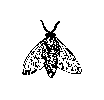
\includegraphics{fly}
%\caption{A sample black and white graphic.}
%\end{figure}
%
%\begin{figure}
%\centering
%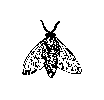
\includegraphics[height=1in, width=1in]{fly}
%\caption{A sample black and white graphic
%that has been resized with the \texttt{includegraphics} command.}
%\end{figure}
%
%
%As was the case with tables, you may want a figure
%that spans two columns.  To do this, and still to
%ensure proper ``floating'' placement of tables, use the environment
%\textbf{figure*} to enclose the figure and its caption.
%and don't forget to end the environment with
%{figure*}, not {figure}!
%
%\begin{figure*}
%\centering
%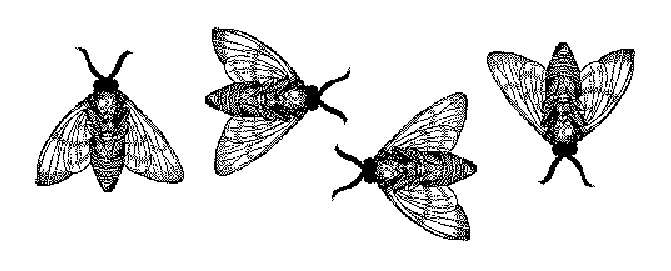
\includegraphics{flies}
%\caption{A sample black and white graphic
%that needs to span two columns of text.}
%\end{figure*}
%
%
%\begin{figure}
%\centering
%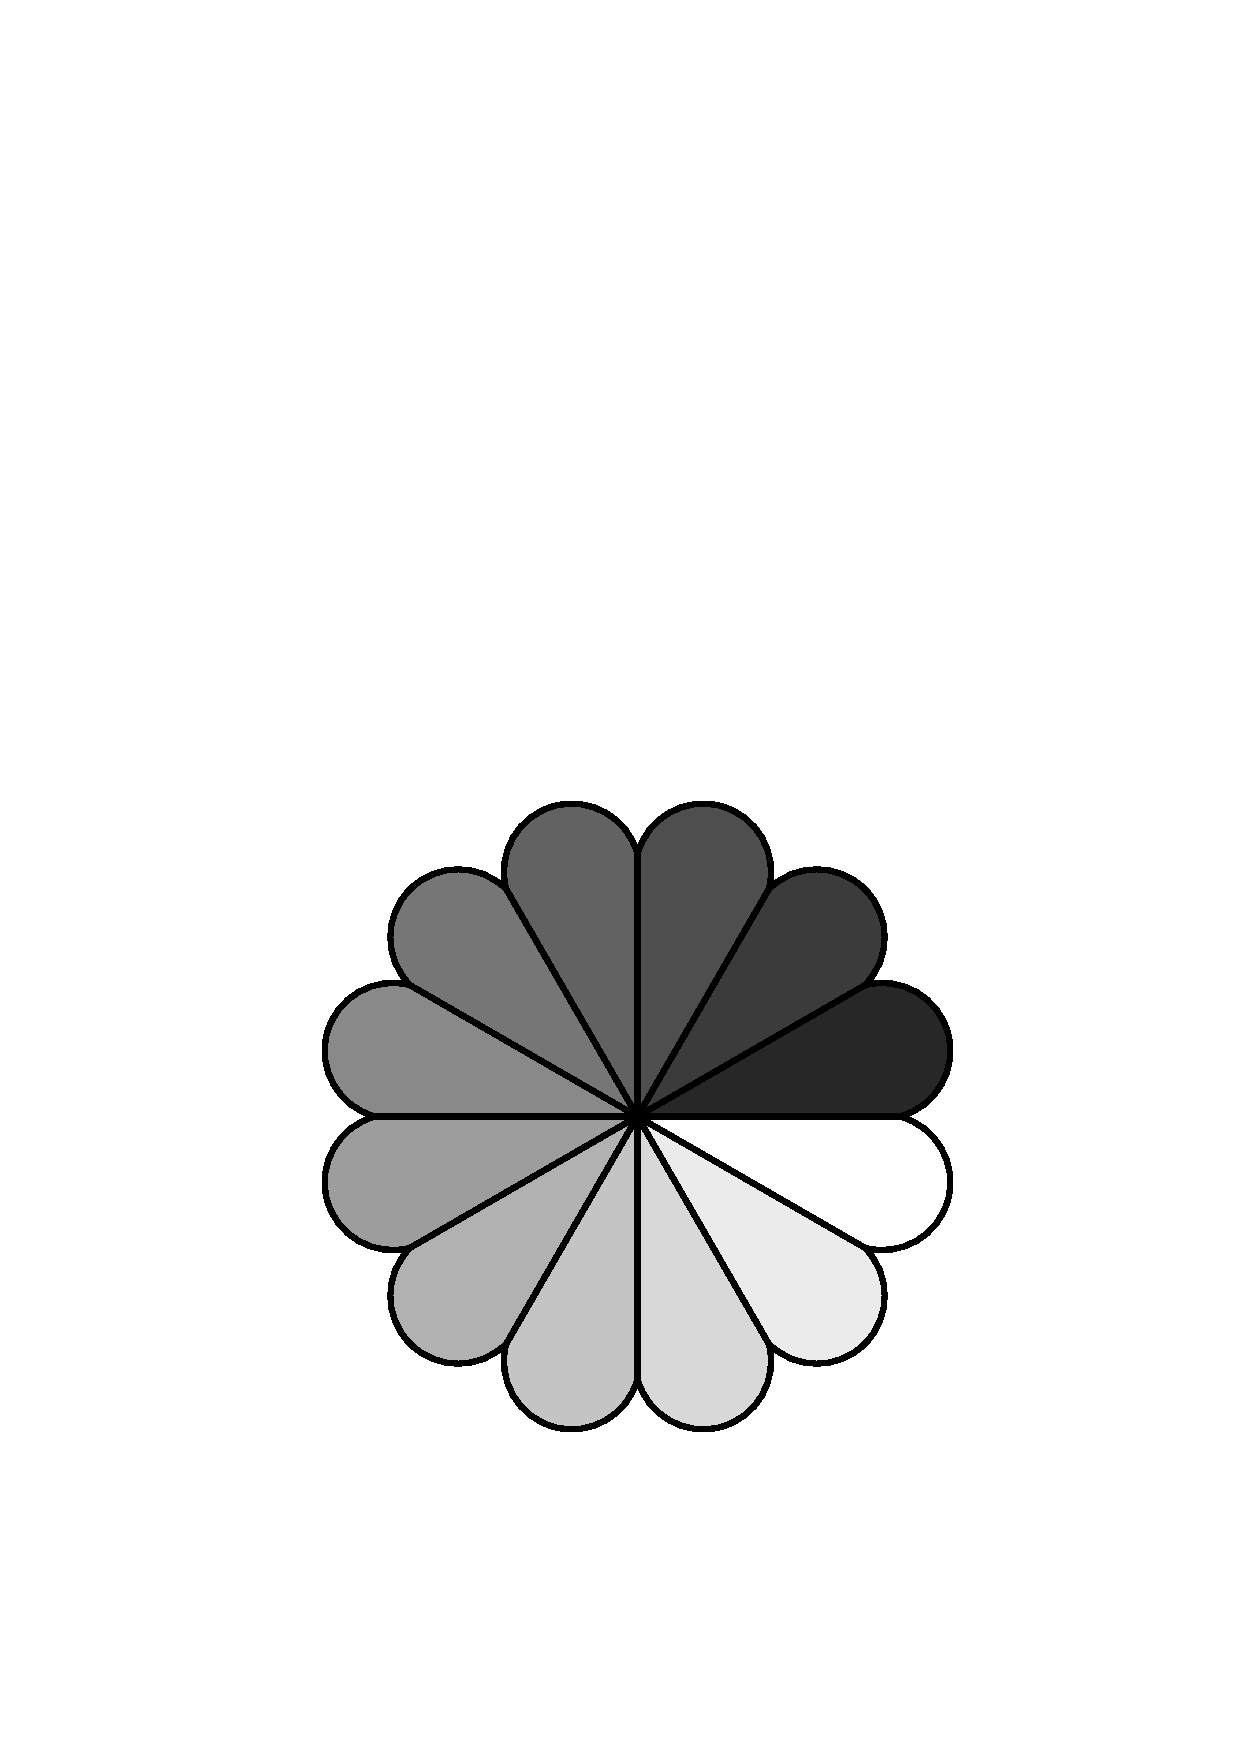
\includegraphics[height=1in, width=1in]{rosette}
%\caption{A sample black and white graphic that has
%been resized with the \texttt{includegraphics} command.}
%\vskip -6pt
%\end{figure}
%
%\subsection{Theorem-like Constructs}
%Other common constructs that may occur in your article are
%the forms for logical constructs like theorems, axioms,
%corollaries and proofs.  There are
%two forms, one produced by the
%command \texttt{{\char'134}newtheorem} and the
%other by the command \texttt{{\char'134}newdef}; perhaps
%the clearest and easiest way to distinguish them is
%to compare the two in the output of this sample document:
%
%This uses the \textbf{theorem} environment, created by
%the\linebreak\texttt{{\char'134}newtheorem} command:
%\newtheorem{theorem}{Theorem}
%\begin{theorem}
%Let $f$ be continuous on $[a,b]$.  If $G$ is
%an antiderivative for $f$ on $[a,b]$, then
%\begin{displaymath}\int^b_af(t)dt = G(b) - G(a).\end{displaymath}
%\end{theorem}
%
%The other uses the \textbf{definition} environment, created
%by the \texttt{{\char'134}newdef} command:
%\newdef{definition}{Definition}
%\begin{definition}
%If $z$ is irrational, then by $e^z$ we mean the
%unique number which has
%logarithm $z$: \begin{displaymath}{\log e^z = z}\end{displaymath}
%\end{definition}
%
%Two lists of constructs that use one of these
%forms is given in the
%\textit{Author's  Guidelines}.
%
%There is one other similar construct environment, which is
%already set up
%for you; i.e. you must \textit{not} use
%a \texttt{{\char'134}newdef} command to
%create it: the \textbf{proof} environment.  Here
%is a example of its use:
%\begin{proof}
%Suppose on the contrary there exists a real number $L$ such that
%\begin{displaymath}
%\lim_{x\rightarrow\infty} \frac{f(x)}{g(x)} = L.
%\end{displaymath}
%Then
%\begin{displaymath}
%l=\lim_{x\rightarrow c} f(x)
%= \lim_{x\rightarrow c}
%\left[ g{x} \cdot \frac{f(x)}{g(x)} \right ]
%= \lim_{x\rightarrow c} g(x) \cdot \lim_{x\rightarrow c}
%\frac{f(x)}{g(x)} = 0\cdot L = 0,
%\end{displaymath}
%which contradicts our assumption that $l\neq 0$.
%\end{proof}
%
%Complete rules about using these environments and using the
%two different creation commands are in the
%\textit{Author's Guide}; please consult it for more
%detailed instructions.  If you need to use another construct,
%not listed therein, which you want to have the same
%formatting as the Theorem
%or the Definition\cite{salas:calculus} shown above,
%use the \texttt{{\char'134}newtheorem} or the
%\texttt{{\char'134}newdef} command,
%respectively, to create it.
%
%\subsection*{A {\secit Caveat} for the \TeX\ Expert}
%Because you have just been given permission to
%use the \texttt{{\char'134}newdef} command to create a
%new form, you might think you can
%use \TeX's \texttt{{\char'134}def} to create a
%new command: \textit{Please refrain from doing this!}
%Remember that your \LaTeX\ source code is primarily intended
%to create camera-ready copy, but may be converted
%to other forms -- e.g. HTML. If you inadvertently omit
%some or all of the \texttt{{\char'134}def}s recompilation will
%be, to say the least, problematic.
%
%\section{Conclusions}
%This paragraph will end the body of this sample document.
%Remember that you might still have Acknowledgments or
%Appendices; brief samples of these
%follow.  There is still the Bibliography to deal with; and
%we will make a disclaimer about that here: with the exception
%of the reference to the \LaTeX\ book, the citations in
%this paper are to articles which have nothing to
%do with the present subject and are used as
%examples only.
%%\end{document}  % This is where a 'short' article might terminate
%
%%ACKNOWLEDGMENTS are optional
%\section{Acknowledgments}
%This section is optional; it is a location for you
%to acknowledge grants, funding, editing assistance and
%what have you.  In the present case, for example, the
%authors would like to thank Gerald Murray of ACM for
%his help in codifying this \textit{Author's Guide}
%and the \textbf{.cls} and \textbf{.tex} files that it describes.

%
% The following two commands are all you need in the
% initial runs of your .tex file to
% produce the bibliography for the citations in your paper.
\bibliographystyle{abbrv}
\bibliography{allrec}  % sigproc.bib is the name of the Bibliography in this case
% You must have a proper ".bib" file
%  and remember to run:
% latex bibtex latex latex
% to resolve all references
%
% ACM needs 'a single self-contained file'!
%
%APPENDICES are optional
%\balancecolumns
%\appendix
%%Appendix A
%\section{Headings in Appendices}
%The rules about hierarchical headings discussed above for
%the body of the article are different in the appendices.
%In the \textbf{appendix} environment, the command
%\textbf{section} is used to
%indicate the start of each Appendix, with alphabetic order
%designation (i.e. the first is A, the second B, etc.) and
%a title (if you include one).  So, if you need
%hierarchical structure
%\textit{within} an Appendix, start with \textbf{subsection} as the
%highest level. Here is an outline of the body of this
%document in Appendix-appropriate form:
%\subsection{Introduction}
%\subsection{The Body of the Paper}
%\subsubsection{Type Changes and  Special Characters}
%\subsubsection{Math Equations}
%\paragraph{Inline (In-text) Equations}
%\paragraph{Display Equations}
%\subsubsection{Citations}
%\subsubsection{Tables}
%\subsubsection{Figures}
%\subsubsection{Theorem-like Constructs}
%\subsubsection*{A Caveat for the \TeX\ Expert}
%\subsection{Conclusions}
%\subsection{Acknowledgments}
%\subsection{Additional Authors}
%This section is inserted by \LaTeX; you do not insert it.
%You just add the names and information in the
%\texttt{{\char'134}additionalauthors} command at the start
%of the document.
%\subsection{References}
%Generated by bibtex from your ~.bib file.  Run latex,
%then bibtex, then latex twice (to resolve references)
%to create the ~.bbl file.  Insert that ~.bbl file into
%the .tex source file and comment out
%the command \texttt{{\char'134}thebibliography}.
%% This next section command marks the start of
%% Appendix B, and does not continue the present hierarchy
%\section{More Help for the Hardy}
%The sig-alternate.cls file itself is chock-full of succinct
%and helpful comments.  If you consider yourself a moderately
%experienced to expert user of \LaTeX, you may find reading
%it useful but please remember not to change it.
%\balancecolumns % GM June 2007
% That's all folks!
 

%\begin{lstlisting}
%-------------------------------- MODULE RYW --------------------------------
%
%EXTENDS Naturals, TLC
%CONSTANT N
%VARIABLE el, op_i, op_j, x_i, x_j, v_i, v_j, W_i, R_j, sip, i, j, el1 , op_i1, op_j1, x_i1, x_j1, v_i1, v_j1, W_i1, R_j1, i1, j1
%
%st == {&lt;&lt;1, "w","x",1&gt;&gt;, &lt;&lt;2, "w","x",2&gt;&gt;, &lt;&lt;3, "r","x",2&gt;&gt;, &lt;&lt;4, "r", "x", 1&gt;&gt;}
%St == {&lt;&lt;1,"w","x",1&gt;&gt;, &lt;&lt;2,"r","x",2&gt;&gt;, &lt;&lt;3,"w","x",2&gt;&gt;, &lt;&lt;4,"r","x",1&gt;&gt;}
%perm == Permutations(st)
%
%Init  ==  /\ el \in st  /\ op_i \in {"r", "w"}  /\ op_j \in {"r", "w"}
%          /\ x_i \in {"x", "y"}  /\ x_j \in {"x", "y"}  /\ i \in 1..999
%          /\ j \in 1..999  /\ v_i \in 1..999  /\ v_j \in 1..999  /\ W_i \in 1..999
%          /\ R_j \in 1..999
%          /\ sip \in {RandomElement(perm) : p \in perm}
%          /\ el1 \in St /\ op_i1 \in {"r", "w"}  /\ op_j1 \in {"r", "w"}
%          /\ x_i1 \in {"x", "y"}  /\ x_j1 \in {"x", "y"}  /\ /\ i1 \in 1..999
%          /\ j1 \in 1..999 /\ v_i1 \in 1..999
%          /\ v_j1 \in 1..999  /\ W_i1 \in 1..999 /\ R_j1 \in 1..999
%
%Next  ==  (/\ el' \in St
%          /\ op_i' = IF el'[2] = "w" THEN el'[2] ELSE "999999999"
%          /\ op_j' = IF el'[2] = "r" THEN el'[2] ELSE "9999999"
%          /\ x_i' = IF op_i' = "w" THEN el'[3] ELSE "999999"
%          /\ x_j' = IF op_j' = "r" THEN el'[3] ELSE "99999"
%          /\ i' = IF op_i' = "w" THEN el'[1] ELSE 999999
%          /\ j' = IF op_j' = "r" THEN el'[1] ELSE 999999
%          /\ v_i' = IF op_i' = "w" THEN el'[4] ELSE 999
%          /\ v_j' = IF op_j' = "r" THEN el'[4] ELSE 999
%          /\ W_i' = IF op_i' = "w" THEN v_i' ELSE 9999
%          /\ R_j' = IF op_j' = "r" THEN v_j' ELSE 9999 )
%          \/ ( el1' \in st
%          /\ op_i1' = IF el1'[2] = "w" THEN el'[2] ELSE "999999999"
%          /\ op_j1' = IF el1'[2] = "r" THEN el'[2] ELSE "9999999"
%          /\ x_i1' = IF op_i1' = "w" THEN el'[3] ELSE "999999"
%          /\ x_j1' = IF op_j' = "r" THEN el'[3] ELSE "99999"
%          /\ i1' = IF op_i1' = "w" THEN el'[1] ELSE 999999
%          /\ j1' = IF op_j1' = "r" THEN el'[1] ELSE 999999
%          /\ v_i1' = IF op_i1' = "w" THEN el'[4] ELSE 999
%          /\ v_j1' = IF op_j1' = "r" THEN el'[4] ELSE 999
%          /\ W_i1' = IF op_i1' = "w" THEN v_i' ELSE 9999
%          /\ R_j1' = IF op_j1' = "r" THEN v_j' ELSE 9999
%          /\ sip' = RandomElement(perm) )
%
%
%LHS == (W_i =&gt; &lt;&gt; R_j) /\ W_i = W_i1 /\ W_i # 9999 /\ R_j # 9999 /\ x_i = x_j /\ (W_i1 =&gt; &lt;&gt; R_j1) /\ R_j1 = R_j1 \*W_i =&gt; &lt;&gt; R_j /\ W_i = R_j /\ W_i # 9999 /\ R_j # 9999 /\ x_i = x_j
%
%RHS == \E s \in sip : [] W_i =&gt; &lt;&gt; R_j  \* /\  PrintT(sip) &lt;&gt; W_i =&gt; &lt;&gt; R_j
%
%Spec  ==  /\ Init /\ [] [Next]_&lt;&lt;el, v_i, v_j, x_i, x_j, op_i, op_j, W_i, R_j, i, j, el1, v_i1, v_j1, x_i1, x_j1, op_i1, op_j1, W_i1, R_j1, i1, j1&gt;&gt;
%
%TypeInvariant  ==  st # {}  \* /\  PrintT(sip)
%
%-----------------------------------------------------------------------
%THEOREM Spec =&gt; [] TypeInvariant /\ LHS \*E_s \/ C
%=============================================================================
%\* Modification History
%\* Last modified Sun Dec 25 17:27:39 GMT 2016 by user
%\* Last modified Mon Dec 12 00:22:23 GMT 2016 by ssidha1
%\* Created Fri Dec 09 12:03:16 GMT 2016 by user
%
%\end{lstlisting}
\section{Appendix}
\subsection{Derivations of Rest of the ConSpec Specifications}\label{sec:restderive}
  %Session Monotonic or Monotonic Read (also referred to as Session Causality or MR) consistency model is
 %another popular consistency model \cite{Chockler2000, Terry:1994:SGW:645792.668302}.
  According to Chockler et al.,
 MR is expressed as: if the condition  (Condition 1) $\mathit{o}^1 \xrightarrow{\sigma} \mathit{o}^2$ holds for a given execution sequence $\sigma$, where both $\mathit{o}^1$ and $\mathit{o}^2$ are read operations,
  there must exist a serialization ${S_p}$, comprising the
   operations $\mathit{o}^1$ and $\mathit{o}^2$, for which the condition (Condition 2)
  $\mathit{o}^1 \xrightarrow{S_p} \mathit{o}^2$ holds.
   Again, following the same logic as in RYW, the above precedence relationships among operations $\mathit{o}^1$ and $\mathit{o}^2$ in Condition 1 can be directly
  expressed in terms of an LTL expression
    $R^{'} F R^{''} \in \mathit{st}$.   Similarly, the expression $\mathit{o}^1 \xrightarrow{S_p} \mathit{o}^2$ in Condition 2
  can be expressed in terms of LTL as $R^{'} F R^{''} \in S_p$. 
    Further, similar to the derivation of RYW,  we can rewrite the expression $R^{'} F R^{''} \in S_p$ in Condition 2 as  $R^{'} \preccurlyeq_{\mathit{st}+w} R^{''}$, thus reducing the above specification  into Equation \ref{eqn:MR}. 
%    Let us consider a sequence of consecutive read operations $R^i$ and $R^j$  in a given
%    session trace $\mathit{st}$, i.e., the condition ${R^i}^{'} F {R^j}^{'} \in \mathit{st}$ holds. Further,
%     consider that there exists two consecutive write operations $w^m$ and $w^n$ in the global session
%    history, i.e., the condition ${W^m}^{''} F {W^n}^{''}  \in \mathcal{S}_t$ holds. According to the definition of MR,
%     if the first read operation $r^i$ returns the
%    result of the later write $w^n$, then either of the following conditions must hold: 1) the read $r^j$ that follows $r^i$ can not return the result
%    written by an earlier read by the earlier write $w^m$, i.e., the condition $\left( {v^i}^{'} = {v^n}^{''} \right) \wedge \big( \left( {v^j}^{'} = {v^m}^{''} \right)$ holds, or 2) the read operation $r^j$ is directly followed by write
%    operation $w^m$, i.e., the condition $\left( {W^m}^{'} F {R^j}^{'} \in \mathcal{S}_t \right) \wedge \left( \not\exists {W^m}^{'} F {W^p}^{'} F {R^j}^{'} \in \mathcal{S}_t \right)$ holds.
%    %The above condition can be expressed in terms of LTL
%%    by the expression $\left( {v^i}^{'} = {v^n}^{''} \right) \wedge \big( \left( {v^j}^{'} = {v^m}^{''} \right)$.
%    The above conditions can be combined together to the anomaly expression for MR, i.e.,
%     $C = \not\exists \big( \left( {R^i}^{'} F {R^j}^{'} \in \mathit{st} \right) \wedge %\left( {\mathit{st}}^{'} \in \mathcal{S}_t \right) \wedge
% \left( {W^m}^{''} F {W^n}^{''}  \in \mathcal{S}_t \right) \\ \big( %\left( {W^m}^{''} F {W^n}^{''} F {R^i}^{'} F {R^j}^{'} \in \mathcal{S}_t \right) \wedge \\
% \left( {v^i}^{'} = {v^n}^{''} \right) \wedge \big( \left( {v^j}^{'} = {v^m}^{''} \right) \vee \big( \left( {W^m}^{'} F {R^j}^{'} \in \mathcal{S}_t \right) \wedge \\ \left( \not\exists {W^m}^{'} F {W^p}^{'} F {R^j}^{'} \in \mathcal{S}_t \right) \big) \big) \big)$.
 %Thus, the ConSpec specification for MR is directly derived from the definition by Chockler et al.
   %\begin{align}%\label{eqn:PL299}
%\begin{split}
%\big(\star \left( W^j(v_l)X^{o}R^k{v_m} \right) \\ \wedge \left( W^n(v_q) X^{o}R^s{v_t} \wedge ( R^k{v_m}F^{o}R^s{v_t} \right) \star \big)^\mathit{po}_{o}
%\\ \rightarrow \big(G\; \star \left( W^n(v_q) X^{o}R^s{v_t} \right)\oplus \\ \left(W^n(v_q) F^{o} W^u(v_x) X^{o} R^s{v_t} \right) \star \big)_{o}^\mathit{st}
%\end{split}
%\end{align}.  $W^n(v_q) X^{o}R^s{v_t}$ implies that the read operation $r^s(o){v_t}$ must return the value $v_x$ written by the write operation $w^n(, ov_q)$. This, in turn, implies $v_t = v_x$.
  %Thus, the above expression can be again rewritten as \begin{align}%\label{eqn:PL299}
%\begin{split}
%\big(\star \left( w^j(v_l)X^{o}r^k{v_m} \right) \wedge \left( w^n(v_q)X^{o}r^s{v_t} \right) \star \big)^\mathit{po}_{o} \\
%\rightarrow \big(G\; \star \left( v_q \gets \left( R^k{v_m}F^{o}R^s{v_t} \right) \right)\oplus \\ \left( v_x \gets \left( W^n(v_q) F^{o} W^u(v_x) X^{o} R^s v_t \right) \right) \star \big)_{o}^\mathit{st}
%\end{split}
%\end{align}.
% Additionally, we also consider a read operation $r^s(o){v_t}$ that reads values written by $w^n(o,v_q)$, i.e., \\ $w^n(o,v_q) X^{o} r^s(o){v_t}$. Then, without violating the above conditions, the above expression can be reduced to the ConSpec expression for MR, given as
% Hence, the above equation can be directly reduced to the equivalent ConSpec expression for MR, which is
% \begin{align}%\label{eqn:PL299}
%\begin{split}
%\forall i, j, k, l, m, n, q, r, s, t \big(\star ( W^j(v_l)X^{o}R^k{v_m} ) \\ \wedge ( W^n(v_q)X^{o}R^s{v_t} ) \wedge ( R^k{v_m}F^{o}R^s{v_t} ) \star \big)^\mathit{po}_{o} \\
%\rightarrow \big(G\; \star %\left( v_t = v_q \right) \wedge
%  (v_t = v_q ) \oplus ( W^n(v_q) F^{o} W^u(v_x) X^{o} R^s{v_t} ) \star \big)_{o}^\mathit{st}.
%\end{split}
%\end{align}.
%$\forall i, j, o, \mathit{st} \; \big( \mathit{Op}^i X \mathit{Op}^j \in \mathit{st}
%\rightarrow \exists S \left( \mathit{Op}^i X \mathit{Op}^j \in S \right) \\ \wedge
%\forall \mathit{st}  \left( \mathit{Op}^j X^o R_k \in \mathit{st} \right) \wedge \left( v^k = v^j  \right) \big)$
\par  Chockler et al. states WFR consistency as: if the condition (Condition 1) 
  $\mathit{o}^1 \xrightarrow{\sigma} \mathit{o}^2$ holds for a given execution sequence $\sigma$ of a read operation
   $\mathit{o}^1$ followed by a write operation  $\mathit{o}^2$, there must exist a serialization ${S_p}$, comprising the
   operations $\mathit{o}^1$ and $\mathit{o}^2$, for which the condition (Condition 2) 
  $\mathit{o}^1 \xrightarrow{S_p} \mathit{o}^2$ must hold.
   As in the case of of our derivations for sRYW and MR, the expressions $\mathit{o}^1 \xrightarrow{\sigma} \mathit{o}^2$,
  and $\mathit{o}^1 \xrightarrow{S_p} \mathit{o}^2$ for Conditions 1 and 2  can be rewritten as LTL expressions
   $R^{'} F W^{''} \in \mathit{st}$ and $R^{'} F W^{''} \in S_p$, respectively.  %, where a session trace $\mathit{st}$ is equivalent to $\sigma$ for the
    %means and purposes of this paper.
 % Thus, the expressions $\left(\mathit{o}^1 \rightarrow \mathit{o}^2\right)^\sigma$ can be rewritten as LTL formula
%  $\left(\mathit{Op}^1 X^{o} \mathit{Op}^2\right)_{o}^\mathit{po}$.
   %Similarly, the expression $\mathit{o}^1 \xrightarrow{S} \mathit{o}^2$ in Condition 2
  %can be expressed in terms of LTL as $R^{'} F W^{''} \in S_p$$. 
  Following from the reasoning of or derivations of  RYW and MR, the expression $R^{'}  F W^{''}  \in S_p$ for Condition 2 can be rewritten in terms of ConSpec as  $R^{'}  \preccurlyeq_{\mathit{st}+w} W^{''}$,  thus reducing the WFR definition to Equation \ref{eqn:WFR}. 
  % Further,
%   since WFR talks about a sequence comprising a read and a write operation, the propositional variable
%   $\mathit{Op}^1$ and   $\mathit{Op}^2$ in both Condition 1 and Condition 2 can safely be  replaced  by new
%   propositional variables  $R^i$ and $W^j$.
%   Further, let us consider consecutive read operations $r^k$ and $r^j$ in a  given session trace, and a write operation $w^i$
%   preceded by a write operation $w^l$.  According to WFR, under the above condition, if the earlier read $r^k$ returns the result of the later write
%   $w^i$, then  one of the following conditions must
%   hold: 1) a later read $r^j$ can not return the result of an earlier write $w^l$, i.e., $ {v^j}^{'} = {v^l}^{'}$, or
%   2) the read $r^j$ must directly succeed the write $w^l$ in the global session history, i.e., $\left( {W^l}^{'} F {R^j}^{'} \in \mathcal{S}_t \right) \wedge \left( \not\exists {W^l}^{'} F {W^m}^{'} F {R^j}^{'} \in \mathcal{S}_t \right)$.
%   Further, let us consider a session trace comprising a sequence of reads $r^i$ and $r^k$ that follows a write operation $w^j$, and a write
%   operation $w^m$ precedes read $r^k$ in the global session history. If $r^i$ reads from $w^j$, $r^k$ reads from $w^m$, and
%    a read operation $r^l$ reads from $w^j$, then one of the following conditions must hold: 1) $r^l$ reads from $w^m$, i.e.,
%     ${v^l}^{''} = {v^j}^{''}$,  or 2) $w^m$ is directly succeeded by $r^l$, i.e., $ \left( {W^m}^{''} F { R^l}^{''} \in \mathcal{S}_t \right) \wedge
%   \left(  \not\exists {W^m}^{''} F {W^n}^{''} F { R^l}^{''} \in \mathcal{S}_t  \right)$. %can be also expressed as: a read operation $r^n$ must not observe
%%    a value that is written by  an earlier read $r^i$ instead of a later write operation $w^j$ in the
%%    execution sequence. %The above condition can be expressed in terms of the LTL expression
%    %$\not\exists  \mathit{st} \left( R^i F W^j F R^n \in \mathit{st} \right) \wedge \left( W^j F R^n \in \mathit{st} \right) \wedge \left( v^n = v^i \right)$.
%     Combining the above
%  conditions, we can derive the ConSpec expression for WFR $ C = \not\exists  \big( %\left( {W^i}^{'} F {R^j}^{'} \in \mathit{st} \right) \wedge
%\left( {R^k}^{'} F {R^j}^{'} \in \mathit{st} \right) \wedge \\
%%\left(  \mathit{st}^{'} \in \mathcal{S}_t \right) \wedge
%\left( {W^l}^{'} F {W^i}^{'} \in \mathcal{S}_t \right) %\big) \\
%\big( \left(  {v^k}^{'} = {v^i}^{'} \right) \wedge \big( \left( {v^j}^{'} = {v^l}^{'} \right) \vee \\
%\big( \left( {W^l}^{'} F {R^j}^{'} \in \mathcal{S}_t \right) \wedge \left( \not\exists {W^l}^{'} F {W^m}^{'} F {R^j}^{'} \in \mathcal{S}_t \right) \big) \big) \big) \wedge \\
% \not\exists \big(  \left(  {W^j}^{''}  F  {R^i}^{''} F {R^k}^{''} \in \mathcal{S}_t \right) \wedge \left(  {W^m}^{''}  F  {R^k}^{''} \in \mathcal{S}_t \right) \wedge \\
% \left( {v^j}^{''} = {v^i}^{''} \right) \wedge \left( {v^m}^{''} = {v^k}^{''} \right)  \wedge \left( {v^l}^{''} = {v^j}^{''} \right)  \big) \big( \left( {v^m}^{''} = {v^l}^{''} \right) \\
%  \vee \big( \left( {W^m}^{''} F { R^l}^{''} \in \mathcal{S}_t \right) \wedge
%   \left(  \not\exists {W^m}^{''} F {W^n}^{''} F { R^l}^{''} \in \mathcal{S}_t  \right)  \big)  \big)$
%   (refer to Equation \ref{eqn:WFR}).
  \par Chockler et al. states the MW consistency model as: if the condition (Condition 1)   $\mathit{o}^1 \xrightarrow{\sigma} \mathit{o}^2$ holds for a given execution sequence $\sigma$ of write operations $\mathit{o}^1$ and $\mathit{o}^2$, there must exist a serialization ${S_p}$, comprising the
   operations $\mathit{o}^1$ and $\mathit{o}^2$, for which the condition (lCondition 2) 
  $\mathit{o}^1 \xrightarrow{S} \mathit{o}^2$ must hold.   Following the same line of reasoning as that of our derivations for RYW, MR, and WFR, the expressions $\mathit{o}^1 \xrightarrow{\sigma} \mathit{o}^2$,
  and $\mathit{o}^1 \xrightarrow{S_p} \mathit{o}^2$  can be rewritten as LTL expressions
   $W^{'} F W^{''} \in \mathit{st}$ and $W^{'} F W^{''} \in S_p$, respectively. 
%  The above precedence relationships among operations $\mathit{o}^1$ and $\mathit{o}^2$ in Condition 1 can be directly
%  expressed in terms of an LTL expression
%    $\mathit{Op}^1 F \mathit{Op}^2 \in \mathit{st}$, where a session trace $\mathit{st}$ is equivalent to $\sigma$ for the
%    means and purposes of this paper.
 % Thus, the expressions $\left(\mathit{o}^1 \rightarrow \mathit{o}^2\right)^\sigma$ can be rewritten as LTL formula
%  $\left(\mathit{Op}^1 X^{o} \mathit{Op}^2\right)_{o}^\mathit{po}$.
%   The expression $\mathit{o}^1 \xrightarrow{Si} \mathit{o}^2$ in Condition 2
%  can be expressed in terms of LTL as $\mathit{Op}^1 F \mathit{Op}^2 \in S_p$,  where
%  $S_p$ is equivalent to $S_p$.  Further,
%   since MW talks about a sequence of write operations, the propositional variable
%   $\mathit{Op}^1$ and   $\mathit{Op}^2$ in both Condition 1 and Condition 2 can safely be  replaced  by new
%   propositional variables  $W^{'}$ and $W^{''}$.
 Exactly like our previous derivations, the expression $W^{'}  F W^{''}  \in S_p$ for Condition 2  can be rewritten as  $W^{'}  \preccurlyeq_{\mathit{st}+w} W^{''}$,  thus reducing the definition into Equation \ref{eqn:MW}. 
%Further, the definition of MW can be also expressed as: a read operation $r^n$ must not observe
%    a value that is written by  an earlier write $w^i$ instead of a later write operation $w^j$ in the
%    execution sequence. The above condition can be expressed in terms of the LTL expression
%    $\not\exists  \mathit{st} \left( W^i F W^j F R^n \in \mathit{st} \right) \wedge \left( v^n = v^i\right)$.
% Let us consider that there exists two consecutive write operations $w^i$ and $w^j$ in a given session
%    trace, i.e., the condition ${W^i}^{''} F {W^j}^{''}  \in \mathit{st}$ holds. A read operation $r^m$
%    cannot read the result of the earlier write operation $w^i$.
% Further, let us consider a sequence of consecutive read operations $r^k$ and $r^l$  in a given
%   global session history $\mathcal{S}_t$, i.e., the condition ${R^k}^{'} F {R^l}^{'} \in \mathcal{S}_t$ holds. According to
%   the definition of MR, if the first read operation $r^k$ returns the
%    result of the later write $w^j$, then the later read $r^l$ that follows $r^k$ can not return the result
%    written by the earlier write $w^i$, i.e., the condition $\left( {v_k}^{''} = {v_j}^{'} \right) \wedge \left( {v_l}^{''} = {v_i}^{'} \right) $
%    must hold. Further, let us consider the read operation $r^k$  reads the result of a preceding write $w^m$, and the read $r^n$ reads the
%    result of a write $w^i$, the write $w^i(x)$ precedes $w^j(y)$ in the given session trace. Then, one of the following
%    conditions must hold: 1) $r^n$ read the result of the write $w^m$, i.e., ${v_m}^{''} = {v_n}^{''}$ or 2) $r^n$ directly follows $w^m$ in the given
%    session trace, i.e., $\left( {W^m}^{'} F {R^n}^{'} \in \mathcal{S}_t \right) \wedge \\
%      \not\exists \left( {W^m}^{'} F {W^p}^{'} F {R^n}^{'} \in \mathcal{S}_t \right)$. Combining the above
%  conditions, we can derive the anomaly expression for MW $C = \not\exists {W^j}^{'} F  {R^m}^{'} \in \mathit{st} \left( {v_m}^{'} = {v_i}^{'} \right)  \wedge \left( \not\exists  {R^k}^{''} F  {R^l}^{''} \in \mathcal{S}_t \right) \\
%   \left( \left( {v_k}^{''} = {v_j}^{'} \right) \wedge \left( {v_l}^{''} = {v_i}^{'} \right) \right) \wedge \not\exists \big( \left( {W^m}(x)^{'} F {R^k}(x)^{'} \in \mathcal{S}_t  \right) \wedge \\
%     \left( {v_m}^{''} = {v_k}^{'} \right) \wedge \left(  {W^i}(x)^{'} F {R^n}(x)^{'} \in \mathcal{S}_t \right) \wedge \left( {v_i}^{'} = {v_n}^{'} \right) \wedge \\
%     \left( {W^i}(x)^{'} F  {W^j}(y)^{'} \in \mathit{st} \right) \wedge \left( {R^l}(y)^{'} F  {R^k}(x)^{'} \in \mathcal{S}_t \right) \big) \\
% \big(  \left( {v_m}^{''} = {v_n}^{''} \right) \vee
% \big( \left( {W^m}^{'} F {R^n}^{'} \in \mathcal{S}_t \right) \wedge \\
%      \not\exists \left( {W^m}^{'} F {W^p}^{'} F {R^n}^{'} \in \mathcal{S}_t \right)  \big)$
%      (refer to Equation \ref{eqn:MW}).
 %The postcondition of Chockler et al. implies that in any serialization order, a read operation $\mathit{o}^j$
% must return the values written by the latest write operations that directly precedes it, namely $\mathit{o}^i$.
% This, in turn, implies $v_l = v_m$ and
% $v_l = v_m$, respectively.
% However, subsequent write operations $\mathit{o}^p$ may alternatively overwrite the
%  values  observed/written by operation $\mathit{o}^k$ . The above conditions may be specified by the
% expressions $\mathit{Op}^j F^{o} \mathit{Op}^p X^{o} \mathit{Op}^k$. Thus, the expression for causal
% consistency can be rewritten as
%  \begin{align}
%  \begin{split}
%\forall i, j, k, l, m, n, p, q \big( \big( \left( \mathit{Op}^j = \left( W^j(v_l) \oplus R^j{v_l} \right) \right) \\
%\wedge \left(   \mathit{Op}^k = \left( W^k(v_m) \oplus R^k{v_m} \right) \right) \wedge \left( \mathit{Op}^p = W^p(v_q)  \right) \big)
% \\ \wedge \big( \left( \left( \mathit{Op}^j F^{o} \mathit{Op}^k \right) \oplus \left( \mathit{Op}^j X^{o} \mathit{Op}^k \right) \right)  \\
% \vee \big( \left( \left( \mathit{Op}^j F^{o} \mathit{Op}^n \right) \oplus \left( \mathit{Op}^j X^{o} \mathit{Op}^n \right) \right)  \\
%\wedge \left( \left( \mathit{Op}^n F^{o} \mathit{Op}^k \right) \oplus \left( \mathit{Op}^n X^{o} \mathit{Op}^j \right) \right) \big) \big) \big)_{o}^\mathit{po} \\
%\rightarrow \big(G\;  \left( v_l = v_m \right) \oplus \left( \mathit{Op}^j F^{o} \mathit{Op}^p X^{o} \mathit{Op}^k \right) \big)_{o}^\mathit{st}.
%\end{split}
% \end{align}
%$\forall i, j, k, l, o, \mathit{st}_x, \mathit{st}_y \big( W^i F W^j \in \mathit{st}_x, \mathit{st}_y
%\\ \rightarrow  \exists S \left( W^i F W^j \in S \right) \wedge
%\\ \wedge \not\exists R^m  \left( W^i F W^j F R^m \in \mathit{st}_x, \mathit{st}_y \right) \\
%\wedge \big( \left( \left( v^m = v^i \in \mathit{st}_x  \right) \wedge \left( v^m = v^j \in \mathit{st}_y
%\right) \right) \\
% \vee \left( \left( v^m = v^j \in \mathit{st}_x  \right) \wedge \left( v^m = v^i \in \mathit{st}_y \right)
% \right) \big) \big)
%$
\par In their definition of Causal consistency, Chockler uses the notion of a 
\emph{direct precedence relation} between operations $\mathit{o}$
 and$\mathit{o}^{'} $ in an execution order $\sigma$, denoted as $\xRightarrow{\sigma}$. The expression $\mathit{o} \xRightarrow{\sigma} \mathit{o}^{'} $
  implies that either of the following conditions must hold: Condition 1) $\mathit{o}^{'} $ is a read operation which returns the values written by a write operation $\mathit{o}$, or Condition 2)  a precedence relationship
exists between $\mathit{o}$  and $\mathit{o}^{'} $  in the execution order $\sigma$ , i.e., the precedence condition 
$\mathit{o} \xrightarrow{\sigma} \mathit{o}^{'} $ holds. Causal consistency specifies: if the precondition holds (i.e., if either Condition 1 or Condition 2 holds) for a given pair of operations $\mathit{o}$  and $\mathit{o}^{'} $ in every client in the system (i.e., for every process $p_i$), then the operations $\mathit{o}$  and $\mathit{o}^{'} $ must occur in the same precedence order in an equivalent legal serialzation $S_p$ of a partial execution $\sigma |i + w$ comprising $\mathit{o}$  and $\mathit{o}^{'} $, i.e., the condition $\mathit{o} \xrightarrow{S_p}\mathit{o}^{'} $ must hold for each client in the system. 
 The above postcondition can be expressed in terms of LTL as  $\exists S_p \left( \forall \mathit{Op}^{'} F \mathit{Op}^{''} \in
S_p \right)$, for each client.  The condition ${\mathit{Op}}^{'}  F {\mathit{Op}}^{''}   \in S_p$ denotes a partial order among ${\mathit{Op}}^{'} $ and ${\mathit{Op}}^{''} $ with respect to each client. Hence, following the same line of reasoning as that  used in our derivation for RYW, the above postcondition can be restated as: must exist a partial order $\preccurlyeq$ comprising which respects the order specified among the operations with respect to each client, i.e., in each observed session trace. Thus, the postcondition reduces to the form ${\mathit{Op}}^{'}  \preccurlyeq {\mathit{Op}}^{''}  $.  Resuming our analysis of the preconditions, Condition 1 in the preconditions can be expressed in the
 form ${\mathit{Op}}^{'} F {\mathit{Op}}^{''}$, since the LTL eventually operator $F$  
  is equivalent to the precedence operator $\xrightarrow{\sigma}$.
 The latter part of the precondition implies read operation $\mathit{o}(x){v}^{'}$ corresponding to the propositional variable ${\mathit{Op}}^{'} $ reads the value
 written by the write $\mathit{o}(x,v)^{''}$ corresponding to the propositional variable  ${\mathit{Op}}^{''}$. The above precondition, comprising a logical disjunction over Condition 1 and 2, can be expressed as $ \left( {\mathit{Op}}^{'} = {W}^{'} \right) \wedge \left( {\mathit{Op}}^{''} = {R}^{''} \right) \wedge
   \left( v = v^{'} \right)$. According to Chockler er al., the precondition of causal consistency specifies that a transitive closure 
must exist over the direct precedence relation $\xRightarrow{\sigma}$, i.e., $\xRightarrow{\star}$ must exist. Thus,
the condition $ {\mathit{Op}}^{'} F {\mathit{Op}}^{''} \vee
 \left( \left( {\mathit{Op}}^{'} = {W}^{'} \right) \wedge \left( {\mathit{Op}}^{''} = {R}^{''} \right) \wedge
   \left( v_i = v_j \right) \right)$ must hold.  However, it directly follows from the Condition 1 in Definition \ref{def:form0} that if the postcondition holds, i.e., if a valid $S_p$ exists comprising $\mathit{o}$  and $\mathit{o}^{'} $ exists,  every operation that satisfies the postcondition must reflect results of prior operations in an equivalent $S_p$. Hence, the postcondition implies the transitivity condition in the precondition. Hence, the above precondition can be rewritten as ${\mathit{Op}}^{'}  F {\mathit{Op}}^{''}  \in \mathit{st}$. % The precondition specifies that operations $\mathit{o}^j$  and $\mathit{o}^k$ are comprised in the execution
%order $\sigma$.  The second precondition which claims
% closure under transitivity of direct precedence relations, we can specify that if $\mathit{o}^i$ directly precedes
% $\mathit{o}^k$, and $\mathit{o}^k$ directly precedes $\mathit{o}^j$, $\mathit{o}^i$ directly precedes
% $\mathit{o}^j$.
%Assuming the transitive closure property specified by the second precondition, the direct precedence
% relation among operations $\mathit{o}^i$ and $\mathit{Op}^j$ can be expressed in terms of LTL as : $\big(\big(  \mathit{Op}^i F \mathit{Op}^j \vee \\
% \exists \mathit{Op}^k \in  \mathit{st} \left( \mathit{Op}^i F \mathit{Op}^k  \wedge
%\mathit{Op}^k F \mathit{Op}^j \right) \big) \\ \vee \big( \left( \mathit{Op}^i = W^i \right) \wedge
%\left( \mathit{Op}^j = R^j \right) \wedge \\ \left( \left( v_i = v_j \right) \vee \exists \mathit{Op}^k \in  \mathit{st}
%\left( \left( v_i = v_k \right)
% \wedge \left( v_k = v_j \right) \right) \big) \right) \big)$.
% The above expression matches the LHS of Equation \ref{eqn:Causal}.
 Thus, Chockler's definition reduces into the specification given in Equation \ref{eqn:Causal}. 
% Additionally, the definition of  Causal consistency requires that the operation $\mathit{o}^j$ must not
% read the result of an earlier write operations $w^m$  instead of $\mathit{o}^i$ such that either of the following
%  conditions are satisfied. The first condition specifies that $r^j$ returns the result of $w^m$, i.e., the condition
%   ${v^j}^{'} = {v^m}^{''}$ holds. The second condition specifies that $r^j$ follows the write $w^m$, such that
%   the condition $\left( {W^m}^{'} F {\mathit{Op}^j}^{'} \in \mathit{st} \right) \wedge
%\left( \not\exists {W^m}^{'} F {W^n}^{'} F {\mathit{Op}^j}^{'} \in \mathit{st} \right)$ holds. %The above condition can be expressed as
%%  $\not\exists  \mathit{st} \left( W^m F \mathit{Op}^i F \mathit{Op}^j \in \mathit{st} \right)
%%\wedge \left( v^j = v^m \right)$.
%  We can combine the above expressions to form Equation \ref{eqn:Causal}, thus reducing it to the form of the anomaly condition, i.e.,
%  $C = \not\exists \big( %\left( \mathit{st}^{'} \in \mathcal{S}_t \right) \wedge
%   \left( {\mathit{Op}^i}^{'} F {\mathit{Op}^j}^{'} \in \mathit{st} \right) \wedge
%   \left( {W^m}^{''} \in \mathcal{S}_t \right) \\
%   \wedge \left( {\mathit{Op}^i}^{'} = {W^i}^{'} \right) \big)
%\big( \left( {W^m}^{''} F {\mathit{Op}^i}^{'}  \in \mathcal{S}_t \right) \wedge
%\big( \left( {v^j}^{'} = {v^m}^{''} \right) \vee \\
% \big( \left( {W^m}^{'} F {\mathit{Op}^j}^{'} \in \mathit{st} \right) \wedge
%\left( \not\exists {W^m}^{'} F {W^n}^{'} F {\mathit{Op}^j}^{'} \in \mathit{st} \right) \big) \big) \big)$
 \par Chockler et al. states Sequential Consistency as: the order of execution among operations comprised in any execution
 sequence of a given client application must match the precedence order in an equivalent legal serialization for the given
 execution sequence. Following the same approach as in previous derivation, %the order  of execution among operations in an execution sequence $\sigma$, 
 %can be given  in terms of a series of LTL expression that express the precedence of successive operations in the sequence.
  the precedence relation between a pair successive operations $\mathit{o}$ and $\mathit{o}^{'}$ in an execution sequence $\sigma$ can be expressed as
   $\mathit{Op}^{'} F \mathit{Op}^{''} \in \mathit{st}$.  %Thus, the above condition can be expressed as: any two operations in an execution
  % sequence must execute in an order that matches the precedence relation among these operations in a legal
  % serialization of the above execution sequence. In other words, any two operations must occur in a session trace in an
   %order that matches the precedence relation of these operations in a legal serialization of those operations.  Hence, this condition can be expressed in terms of LTL as
  % $\mathit{Op}^{'} F \mathit{Op}^{''} \in \mathit{st}
  SC requires that an equivalent legal serialization must exist comprising operations performed by all clients in the system which matches the precedence among the operations $\mathit{o}$ and $\mathit{o}^{'}$.  We denote such a legal serialization as $S_c$, the subscript $c$ denotes that the serialization corresponds to a global execution restricted to operations from a given client (refer to the definition of $S_c$ in Equation \ref{def:clientser}). Hence, the postcondition can be expressed as $ \exists S_c \left( \mathit{Op}^{'} F \mathit{Op}^{''} \in S_c \right)$. %, where $S_c$ denotes an equivalent legal serialization of a global execution restricted to operations from the given client (refer to the definition of $S_c$ in Equation \ref{def:clientser}). 
  As in our previous derivations, the above postcondition can be expressed as ${\mathit{Op}}^{'}  \preccurlyeq {\mathit{Op}}^{''}  \in S_c$.  Further, since the condition ${\mathit{Op}}^{'}  F {\mathit{Op}}^{''}  \in S_c$ implies a total order $\prec$ among ${\mathit{o}}(x,v)^{'} $ and ${\mathit{o}}(x,v^{'})^{''}$, we can replace the partial order symbol $\preccurlyeq$ with $\prec$. This does not cause any loss of information since a total order is a special case of a partial order, i.e., ${\mathit{Op}}^{'}  \prec {\mathit{Op}}^{''}$  implies $\left( {\mathit{Op}}^{'} \preccurlyeq {\mathit{Op}}^{''} \right) \vee \left( {\mathit{Op}}^{''}  \preccurlyeq {\mathit{Op}}^{'}\right)$. Hence, we can rewrite the above postcondition as  ${\mathit{Op}}^{'}  \prec {\mathit{Op}}^{''} $. Thus, Chockler's definition of SC reduces into the specification given in Equation \ref{eqn:SC}. 
% Additionally, consider that a read operations $r^j$ follows a write operation $w^i$ in a given session
% trace. Consider a read operation $r_k$ follows $r^j$ in the global session history. Strict serializability
% requires that the later read $r^k$ can not read the result of the write $w^i$ if the earlier read $r^j$ did not observe it,
% i.e., the condition $\left( {W^i}^{'} F {R^j}^{'} \in \mathit{st} \right) \wedge
% \left( {R^j}^{''} F {R^k}^{''} \in \mathcal{S}_t \right) \big)
% \big(  \left( {v^k}^{''} = {v^i}^{'} \right) \wedge   \left( {v^j}^{'} \not= {v^i}^{'} \right) \big)$ must hold.
% Further, consider that a read operation $r^l$ follows the above sequence of write and reads in the global session history,
% i.e., $ \left( {\mathit{Op}^i}^{'}  F {W^j}^{'} F  {R^k}^{'} \in \mathit{st} \right) \wedge
%  \left( {\mathit{Op}^i}^{'} F {W^j}^{''}   F  {R^k}^{'}  F  {R^l}^{'} \in \mathcal{S}_t \right)$. In that case,
%  among the reads following $w^j$ the later read $r^l$ can not observe the result of $w^j$ if the earlier read $r^k$ did not
%   observed it, i.e., \\ $\not\exists \big(  \left( {\mathit{Op}^i}^{'} = {W^i}^{'}  \oplus {R^i}^{'}  \right) \wedge  \left( {\mathit{Op}^i}^{'}  F {W^j}^{'} F  {R^k}^{'} \in \mathit{st} \right) \wedge \\
%  \left( {\mathit{Op}^i}^{'} F {W^j}^{''}   F  {R^k}^{'}  F  {R^l}^{'} \in \mathcal{S}_t \right) \big)
% \big(  \left( {v^l}^{''} = {v^j}^{'} \right) \wedge   \left( {v^k}^{''} = {v^i}^{'} \right) \big)$.
%  %must always observe the result
%% of the latest operation preceding $r_k$. This condition can be expressed in terms of LTL as
%% $\forall \mathit{st}  \left( \mathit{Op}^j X^o R^k \in \mathit{st} \right) \wedge \left( v^k = v^j  \right)$
%  Combining the above
%  conditions, we can derive the anomaly expression for strict serializability, i.e., $C = \not\exists \big( \left( {W^i}^{'} F {R^j}^{'} \in \mathit{st} \right) \\
%   \wedge \left( {R^j}^{''} F {R^k}^{''} \in \mathcal{S}_t \right) \big)
% \big(  \left( {v^k}^{''} = {v^i}^{'} \right) \wedge   \left( {v^j}^{'} \not= {v^i}^{'} \right) \big) \wedge \\
% \not\exists \big(  \left( {\mathit{Op}^i}^{'} = {W^i}^{'}  \oplus {R^i}^{'}  \right) \wedge  \left( {\mathit{Op}^i}^{'}  F {W^j}^{'} F  {R^k}^{'} \in \mathit{st} \right) \wedge \\
%  \left( {\mathit{Op}^i}^{'} F {W^j}^{''}   F  {R^k}^{'}  F  {R^l}^{'} \in \mathcal{S}_t \right) \big)
% \big(  \left( {v^l}^{''} = {v^j}^{'} \right) \wedge   \left( {v^k}^{''} = {v^i}^{'} \right) \big)$ %\wedge
%% \not\exists \big( \left( {\mathit{Op}}^{'} F {W^j}^{'} F {R^k}^{'} \in \mathit{st} \right) \wedge \\
%% \left( {W^i}^{'} F {W^j}^{'} F {R^k}^{''} F {R^l}^{l'} \in \mathcal{S}_t \right) \big)
%% \big(  \left( {v^l}^{''} = {v^j}^{'} \right) \wedge   \left( {v^k}^{'} \not= {v^i}^{'} \right) \big)$
% (refer to Equation \ref{eqn:Strict}).

 \par Goodman\textquotesingle s Processor consistency (PC) specifies that result of a preceding operation invoked from a given client must be observed in all processors before result of a
 succeeding operation can be observed in any processor (or client application).  In other words, the order in which any pair of  writes, invoked from a particular client, are observed in session traces of all other clients must always respect the invocation order of the above operations. Reads against  write operations should
  view the results of the writes
  according to the invocation order of these writes in a client application. Following the same approach as before, the ConSpec specification for PC can be directly derived from the definition of Goodman\textquotesingle s PC provided by Ahamad et al. \cite{Ahamad:1993:PPC:165231.165264}.  
 %PC talks about preserving the order of operations executed by individual processors (or client applications). 
 According to the above definition, there must exist a valid legal serialization for a partial execution  $\sigma |i + w$, which we denote as $S_p$, which must satisfy the following conditions. Condition 1 states: every pair of write operations $w(x,v)$ and $w^{'}(y,v^{'})$ in a system must occur in $S_p$ in the same precedence order as the invocation order of $w(x,v)$ and $w^{'}(y,v^{'})$ in a process $p$ which invokes $w(x,v)$ and $w^{'}(y,v^{'})$.  Ahamad et al. expresses Condition 1 as:  $\mathit{o}^1 \xrightarrow{\sigma} \mathit{o}^2$ implies $\mathit{o}^1 \xrightarrow{S_p} \mathit{o}^2$. In this paper, we refer to a processor  $p$ as a client $\mathit{Cl}$, and the session trace comprising the results observed by  $\mathit{Cl}$ is denoted as $\mathit{st}$. Hence, in our case, Condition 1 implies that the order among $w(x,v)$ and $ w^{'}(y,v^{'})$ invoked by in any valid legal serialization $S_p$ comprising operations performed by a  client $\mathit{Cl}$ must match the precedence order of $w(x,v)$ and  $w^{'}(y,v^{'})$ in a session trace $\mathit{st}$ observed by $\mathit{Cl}$. Following the same line of reasoning as in the previous derivations, we can express a valid legal serialization $S_p$ for a given client $\mathit{Cl}$ in terms of a partial order $\preccurlyeq(x)_{\mathit{st}+w}$ comprising all operations in a session trace $\mathit{st}$ for $\mathit{Cl}$ plus writes from all other clients. Condition 2 states: all writes to a given object in a system must follow an identical precedence order in valid legal serializations for all clients in the system. Imposing the restrictions of Condition 2 on a valid partial order that satisfies Condition 1, precedence order among any pair of writes in all valid partial order corresponding to partial executions of  all clients in a system must match the invocation order of the writes. It follows trivially from the definition of a session that the precedence order among $w(x,v)$ and  $w^{'}(y,v^{'})$ in a session trace $\mathit{st}$ observed by a client $\mathit{Cl}$ is equivalent to the invocation order of  $w(x,v)$ and  $w^{'}(y,v^{'})$ in $\mathit{Cl}$. In that light, the invocation order of a pair of writes  $w(x,v)$ and  $w^{'}(y,v^{'})$ invoked from a client $\mathit{Cl}$ can be expressed, in terms of LTL, as $W^{'}(x) F W^{''} (y) \in \mathit{st} $. We denote $ \preccurlyeq_{\mathit{st}+w}$ and $ \preccurlyeq_{{st}^{'}+w}$ as partial orders restricted to operations performed by clients $\mathit{Cl}$ and $\mathit{Cl}^{'}$ and writes from all other clients, respectively.  Then, according to  Condition 1 and Condition 2, the precedence order among $w(x,v)$ and  $w^{'}(y,v^{'})$ in the partial orders  $\preccurlyeq_{\mathit{st}+w}$ and $ \preccurlyeq_{{st}^{'}+w}$ must match the precedence order  $W^{'}(x) F W^{''} (y) \in \mathit{st} $.  %\\
%E^{s} = C =   \forall \mathit{st} \in \mathcal{S}_t \not\exists \big( \left(  {W^i}^{'}, {W^j}^{'} \in \mathit{st}  \right)
%\wedge \left( {R^k}^{'}, {R^l}^{'} \in \mathcal{S}_t \right) \big) \\
%\big( \left( {W^i}^{'} F {W^j}^{'} \in \mathit{st} \right) \wedge
%   \left( {R^k}^{'} F {R^l}^{'} \in \mathcal{S}_t \right) \wedge
%  \left( v_k^{''} = v_j^{'} \right)  \wedge \\
%  \left( v_l^{'} = v_i^{'} \right) \big) \wedge
%  \not\exists \left( {W^i}^{'}, {R^j}^{'}, {R^k}^{'}, {W^l}^{'}  \in \mathit{st}  \right)
%  \big( \left( {R^k}^{'} F {R^j}^{'} \in \mathit{st} \right) \\ \wedge
%\left( {W^l}^{'} F {W^i}^{'} \in \mathcal{S}_t \right) \wedge  
% \left(  {v^k}^{'} = {v^i}^{'} \right) \wedge \big( \left( {v^j}^{'} = {v^l}^{'} \right) \vee \\
%\big( \left( {W^l}^{'} F {R^j}^{'} \in \mathcal{S}_t \right) \wedge
% \left( \not\exists {W^l}^{'} F {W^m}^{'} F {R^j}^{'} \in \mathcal{S}_t \right) \big) \big) \big)
%E^s = \left( \mathcal{O}, \preccurlyeq \right), 
%$\forall x, y, \mathit{st} \in \mathcal{S}_t  \left( {\mathit{Op}}^{'}(x) F {\mathit{Op}}^{''} (y) \in \mathit{st} \right)  \rightarrow \left( {\mathit{Op}}^{'}(x) \preccurlyeq {\mathit{Op}}^{''} (y) \right),$  where $ \preccurlyeq$ is a partial order over operations across all data objects with respect to a given global session trace $ \mathcal{S}_t$.
Thus, PC can be expressed as $\forall x, y, \mathit{st}, \mathit{st}^{'} \in \mathcal{S}_t  \big( \left( W^{'}(x) F W^{''} (y) \in \mathit{st} \right) \rightarrow  \left(  \left( W^{'}(x) \preccurlyeq_{\mathit{st}+w} W^{''} (y)   \right) \wedge  \left( W^{'}(x)  \preccurlyeq_{{st}^{'}+w}  W^{''} (y)  \right) \right) \big)$.   The partial order relations $  \left( W^{'}(x) \preccurlyeq_{\mathit{st}+w} W^{''} (y)   \right)$ and $ \left( W^{'}(x)  \preccurlyeq_{{st}^{'}+w}  W^{''} (y)  \right)$ can be expressed in terms of the corresponding partial order sets $\left( \mathcal{O}, \preccurlyeq_{\mathit{st}+w} \right)$  and $\left( \mathcal{O}, \preccurlyeq_{{st}^{'}+w} \right)$. By that reasoning, the condition $ \left( W^{'}(x) \preccurlyeq_{\mathit{st}+w} W^{''} (y)   \right) \wedge  \left( W^{'}(x)  \preccurlyeq_{{st}^{'}+w}  W^{''} (y)  \right) $ can be expressed in terms of an intersection $\left( \mathcal{O}, \preccurlyeq^{'} \right)$ of the partial order sets  $\left( \mathcal{O}, \preccurlyeq_{\mathit{st}+w} \right)$  and $\left( \mathcal{O}, \preccurlyeq_{{st}^{'}+w} \right)$, where $ \preccurlyeq^{'} $ denotes the partial order relation  among elements of the new partial order set formed out of the intersection of $\left( \mathcal{O}, \preccurlyeq_{\mathit{st}+w} \right)$  and $\left( \mathcal{O}, \preccurlyeq_{{st}^{'}+w} \right)$.  Thus, the definitions of Ahmad et al. directly reduces to the expression given in Equation \ref{eqn:PC}.
\par Total Store Order (TSO) originally specified by Owens et al. \cite{Owens:2009:BXM:1616077.1616107}, where it was intended to serve as  a memory model for the existing x86 multiprocessor architecture. The axiomatic form of the TSO definition by Owens et al. is based on notations and mechanisms that are very specific to the internal protocol of the x86 architecture. Hence, instead of deriving our definitions directly from the axiomatic model, we first extract the substance of the model and interpret it in terms of a prose, using generalised notations, as follows. A read operation performed by a given client on a given data object can not return the result of write on the same object by a different client unless the former write has been observed by all clients. 
The above condition implies that partial orders for any session trace $\mathit{st}$ and $\mathit{st}^{'}$ must preserve the precedence among writes $ w(x,v)$  and $w^{'''}(x,v^{'''}$ to a  common data object $x$ with resect to succeeding reads.  
Consider an execution sequence comprising $w(x,v)$ followed by a read $r^{'}(x,v^{'})$, observed in a local session trace $\mathit{st}^{'}$. In another session trace $\mathit{st}^{'}$), a read operation $r^{''}(x)$  is  followed by a write $w^{'''}(x,v^{'''})$. 
According to TSO, in a valid global session trace $\mathcal{S}_t$, the read $r^{'}(x,v^{'})$ can not return the value written by $w^{'''}(x,v^{'''})$ before $r^{''}(x)$ returns the result of $w(x,v)$.  For such an $\mathcal{S}_t$  there must exist a valid legal serialization, comprising operations from each client,  where $w(x,v)$ occurs before $w^{'''}(x,v^{'''})$., i.e., there must exist a valid legal serializations for each session trace that orders $w(x,v)$ occurs before $w^{'''}(x,v^{'''})$.  In other words, a valid legal seriallizaton for partial execution of each client (i.e., for each session trace corresponding to the respective clients) must apply writes to each data object in the same precedence order.  Using the same approach that used in the prior derivations, the above condition of a valid legal serialization can be restated in terms of valid partial orders, i.e.,  there must exist valid partial orders $\preccurlyeq(x)_{{st}^{'}}$ and $\preccurlyeq(x)_{{st}}$ over operations comprised in the session traces $\mathit{st}$ and $\mathit{st}^{'}$ that order writes to each data object according to an identical  precedence order.  
  Thus, TSO is expressed as follows.
 $E^s = \forall x, \mathit{st}, \mathit{st}^{'} \in \mathcal{S}_t, w(x,v), r^{'}(x,v^{'}), r^{''}(x), w^{'''}(x,v^{'''}) \in \mathcal{O}  \big( \left( W^{'}(x) F R^{''} (x) \in \mathit{st} \right)  \wedge  \left( \mathit{R}^{'''}(x) F W^{''''} (x) \in \mathit{st}^{'} \right)  \wedge \left( v^{''} = v \right) \wedge \left( v^{'''} = v^{'} \right)  \big) \rightarrow   \big( \left( W^{'}(x) \preccurlyeq(x)_{st} W^{'''} (x) \right) \wedge \left( W^{'}(x) \preccurlyeq(x)_{{st}^{'}} W^{'''} (x) \right)  \big) \big).$
  TSO can be expressed in terms of an intersection of the partial order sets  $\left( \mathcal{O}, \preccurlyeq(x)_{st} \right)$  and $\left( \mathcal{O}, \preccurlyeq(x)_{{st}^{'}} \right)$, where $\preccurlyeq(x)^{'}$  denotes a partial order among elements  of the intersection-set comprising an intersection of the partial order sets $\left( \mathcal{O}, \preccurlyeq(x)_{st} \right)$  and $\left( \mathcal{O}, \preccurlyeq(x)_{{st}^{'}} \right)$. %In any two executions of a sequence of operations by two processors (or client applications), a pair of writes on a common system object $x$ must be executed in the same precedence order.  %serializations ${S_p}_i$ and ${S_p}_j$, the write operations on common storage system objects in ${S_p}_i$ and
% ${S_p}_j$ must be executed in the same order, i.e., ${S_p}_i|w$ = ${S_p}_j|w$.
 Thus,  the above expression for TSO can be reduced to the ConSpec form $E^s = \forall x, \mathit{st}, \mathit{st}^{'} \in \mathcal{S}_t, w(x,v), r^{'}(x,v^{'}), r^{''}(x), w^{'''}(x,v^{'''}) \in \mathcal{O}  \big( \left( W^{'}(x) F R^{''} (x) \in \mathit{st} \right)  \wedge  \left( \mathit{R}^{'''}(x) F W^{''''} (x) \in \mathit{st}^{'} \right)  \wedge \left( v^{''} = v \right) \wedge \left( v^{'''} = v^{'} \right)  \big) \rightarrow   \big( \left( W^{'}(x) \preccurlyeq(x)_{st} W^{'''} (x) \right) \wedge \left( W^{'}(x) \preccurlyeq(x)_{{st}^{'}} W^{'''} (x) \right)  \big).
$. 

%, i.e., there must exist a common serialization comprising all operations executed from the
% client applications which contains the above writes executed in a particular order. This condition can be expressed in terms of LTL as
% $W^i F W^j \in \mathit{st}_x, \mathit{st}_y \rightarrow  \exists S \left( W^i F W^j \in S \right)$.
% Let us consider a given sequence of operations $w^i$ and $r^j$ in any given session trace, whee $r^j$ does not return
%  the result of $w^i$. Further, consider a read operation $r^k$ that executes between  $w^i$ and $r^j$ in the
%  global session history. If the read $r^k$ also does not return the result of $w^i$, there can not exceed a write operation
%  $w^l$ that precedes the write $w^i$, such that one of the following conditions hold: 1) $r^i$ returns the result of $w^l$,
%  i.e., ${v^j}^{'} = {v^l}^{'}$, or 2) $r^i$ directly follows $w^l$, i.e., $\left( {W^l}^{'} F {R^j}^{'} \in \mathcal{S}_t \right) \wedge
% \left( \not\exists {W^l}^{'} F {W^m}^{'} F {R^j}^{'} \in \mathcal{S}_t \right)$.
% that must not observe the sequence
% of writes executing in  a different order in  two different session traces $\mathit{st}_x$ and $\mathit{st}_y$.% The above
%  condition can be expressed as
% $\not\exists R^m  \left( W^i F W^j F R^m \in \mathit{st}_x, \mathit{st}_y \right) \\
%\wedge \big( \left( \left( v^m = v^i \in \mathit{st}_x  \right) \wedge \left( v^m = v^j \in \mathit{st}_y
%\right) \right) \\
% \vee \left( \left( v^m = v^j \in \mathit{st}_x  \right) \wedge \left( v^m = v^i \in \mathit{st}_y \right)
% \right) \big) $.
% The above conditions can be combined to form the condition of TSO $C = \forall \mathit{st}, \mathcal{S}_t \; \big( \not\exists \big( \left({W^i}(x)^{'} \in \mathit{st} \right) \wedge
% \left({R^j}(x)^{''} \in \mathit{st}^{'} \right) \wedge \\
%  \left( {W^i}^{'}(x) F {R^j}^{''}(x) \in \mathcal{S}_t  \right) \wedge \left( {v_j}^{''} \not= {v_i}^{'} \right) \big) \\
%  \big( \not\exists \big( \left({R^k}(x)^{'} \in \mathit{st}^{'} \right) \wedge \left( {R^k}^{''}(x) F {R^j}^{''}(x) \in \mathcal{S}_t  \right)   \big)  \\
%  \left( {v_k}^{''} \not= {v_i}^{'} \right) \big) \wedge
% \not\exists  \big( %\left( {W^i}^{'} F {R^j}^{'} \in \mathit{st} \right) \wedge
%\left( {R^k}^{'} F {R^j}^{'} \in \mathit{st} \right) \wedge
%%\left(  \mathit{st}^{'} \in \mathcal{S}_t \right) \wedge
%\left( {W^l}^{'} F {W^i}^{'} \in \mathcal{S}_t \right) \\ %\big) \\
%\big( \left(  {v^k}^{'} = {v^i}^{'} \right) \wedge \big( \left( {v^j}^{'} = {v^l}^{'} \right) \vee
%\big( \left( {W^l}^{'} F {R^j}^{'} \in \mathcal{S}_t \right) \wedge \\
% \left( \not\exists {W^l}^{'} F {W^m}^{'} F {R^j}^{'} \in \mathcal{S}_t \right) \big) \big) \big)$.  
% The existential quantification over each of the LTL and first order logic expressions comprised in the above expression for $E^s$ can be rewritten as partial orders over the global session trace $\mathcal{S}_t$. 
%The above expression can be rewritten as follows. 
% $E^s = \forall \mathit{st}, \mathcal{S}_t \; \big( \not\exists \big( \left({W^i}(x)^{'} \in \mathit{st} \right) \wedge
% \left({R^j}(x)^{''} \in \mathit{st}^{'} \right) \wedge \\
%  \left( {W^i}^{'}(x) \preccurlyeq^{'}(x) {R^j}^{''}(x)  \right) \wedge \left( {R^j}^{''}(x) \preccurlyeq^{''}(x) {W^i}^{'}(x) \right) \big) \\
%  \big( \not\exists \big( \left({R^k}(x)^{'} \in \mathit{st}^{'} \right) \wedge \left( {R^k}^{''}(x)  \preccurlyeq^{'''}(x) {R^j}^{''}(x) \right)   \big)  \\
%  \left( {R^k}(x)^{'} \preccurlyeq^{''''}(x) {W^i}^{'}(x) \right) \big) \wedge
% \not\exists  \big( %\left( {W^i}^{'} F {R^j}^{'} \in \mathit{st} \right) \wedge
%\left( {R^k}^{'} \preccurlyeq^{''''}(x) {R^j}^{'} \right) \wedge \\
%%\left(  \mathit{st}^{'} \in \mathcal{S}_t \right) \wedge
%\left( {W^l}^{'} \preccurlyeq^{''''}(x) {W^i}^{'} \in \mathcal{S}_t \right)  %\big) \\
%\big( \left(   {R^k}^{'} \preccurlyeq^{''''}(x) {W^i}^{'}  \right) \\ \wedge \big( \left( {W^i}^{'}  \preccurlyeq^{'''''}(x)  {W^l}^{'} \right) \vee
%\big( \left( {W^l}^{'} \preccurlyeq^{'''''}(x) {R^j}^{'} \right) \wedge \\
% \left( \not\exists {W^l}^{'} \preccurlyeq^{'''''}(x) {W^m}^{'} \preccurlyeq^{''''''}(x) {R^j}^{'} \right) \big) \big) \big),$
% where each of the temporal and first order logic operators in the above expression are replaced by equivalent partial orders $\preccurlyeq^{'}(x), \preccurlyeq^{''}(x)...$  over $\mathcal{S}_t$, defined with respect to a given object $x$. The above expression can be further rewritten as $E^s = \left( \mathcal{S}_t, \preccurlyeq^{'}(x) \right) R ... R^{'} \left( \mathcal{S}_t, \preccurlyeq^{''}(x)\right), $ where $R, R^{'}, ... $ are binary relations, like $\vee, 
% \wedge, $ etc., composing the above partial order orders.  This expression can again be rewritten as 
%where $ \mathit{Si} $ is an equivalent legal serialization for a global execution comprising all clients executing in the system, defined in Equation \ref{def:ser}. The above expression can be trivially rewritten as Equation \ref{eqn:TSO}. % further rewritten in terms of a partial order $ \preccurlyeq(x)$ over a given object $x$ as $E^s = \forall x, \mathit{st}, \mathit{st}^{'} \in \mathcal{S}_t \not\exists \mathit{o}(x), \mathit{o}^{'}(x), \mathit{o}^{''}(x), \mathit{o}^{'''}(x) \in \mathcal{O}  \big( \left( \mathit{Op}^{'}(x) F \mathit{Op}^{''} (x) \in \mathit{st} \right)  \vee \big(  \left( \mathit{Op}^{'}(x) F \mathit{Op}^{'''} (x) \in \mathit{st} \right)  \wedge \\
% \left( \mathit{Op}^{''}(x) F \mathit{Op}^{''''} (x) \in \mathit{st}^{'} \right)  \wedge \left( v^{''} = v \right) \wedge \left( v^{'} = v^{'''} \right)  \big) \big) \rightarrow   \left( \mathit{Op}^{'}(x) \preccurlyeq(x) \mathit{Op}^{''} (x) \right),$
  % where $ \preccurlyeq(x)$ is a partial order over a given object $x$ with respect to a given global session trace $ \mathcal{S}_t$.
  %Thus, the ConSpec expression for TSO is derived as follows.
%   Any
%  two write operations with read operations following them must occur in the same order for all executions,
%  irrespective of the store where they are executed. Consider that there exists two write operations
%  $w^j(o,v_l)$ and $w^n(o,v_q)$, with two corresponding read operations $r^k(o){v_m}$ and $r^s(o){v_t}$, such
%  that  conditions $w^j(o,v_l)X^{o}r^k(o){v_m}$ and $w^n(o,v_q)X^{o}r^s(o){v_t}$ hold.
% Following the same line of reasoning as that used in the case of Causal consistency, the following condition
%  must hold:
%  \\ $\forall i, j, o, \mathit{st}, S \; \big( \mathit{Op}^i X W^j \in \mathit{st}
%\rightarrow \\ \forall S \left( \mathit{Op}^i X W^j \in S \right)
%\wedge \not\exists R^k  \left( \mathit{Op}^i X^o W^j X^o R^k \in \mathit{st} \right) \\ \wedge \left( v^k = v^i  \right) \big)
%$.
 %Also, the ConSpec expression for strict
% serializability follows directly from its definition.
%It states that  any serialization of a sequence of operations
%  executed by a processor must observe an identical order of execution among operations. This, in turn, is expressed using Equation
 %\ref{eqn:Strict}.
  %The specification for Write Follows Read consistency (see Equation \ref{eqn:WFR}) is also derived using similar line of reasoning.
%\par The ConSpec specifications for the isolation levels are derived from the definitions by Adya et al.
%\cite{DBLP:conf/icde/AdyaLO00}.  Here, we show that the isolation specifications in ConSpec, given in
%Equations \ref{eqn:PL1}, \ref{eqn:PL2}, \ref{eqn:PL3}, and \ref{eqn:PL299}, follow directly from the
%definitions of isolation levels PL-1, PL-2, PL-3, and PL-2.99 \cite{DBLP:conf/icde/AdyaLO00}. We analyze the
%ConSpec Equations, and demonstrate their equivalence to the definitions of  \cite{DBLP:conf/icde/AdyaLO00}, as
%follows.
%\par  The PL-1 specification states that the anomaly G0 must be proscribed in any session trace collected
%for the execution of a client application. G0 specifies that there can not be any directed cycle in the
%dependency graph corresponding to an execution of a pair of transactions, comprising entirely of write dependency edges.
%%The
%% condition can be avoided if the write dependencies are preserved in any execution of a given client
%% application, i.e., if any pair of write operations are executed in order. The LHS of
%%  Equation \ref{eqn:PL1}, i.e., the expression $W^i_\mathit{tx} F W^j_\mathit{tx} \in \mathit{st}$
%%  denotes the above precondition with respect to a given session trace $\mathit{st}$ comprising any two
%%  write operations $w^i_{tx}$ and $w^j_{tx}$. PL-1 specifies that any session trace must
%%  comprise the above write operations in the same order. This, in turn, implies that the write operation
%%  $w^j_{tx}$ in the session trace $\mathit{st}$ must overwrite the value written by the write operation $w^i_{tx}$, i.e.,
%%  $r^k_{tx}$ that follows the write operation $w^j_{tx}$ must not return the value $v_i$ written by an earlier
%%   write. The above condition can be expressed as $\not\exists R^k_\mathit{tx} \in \mathit{st} \left( W^i_\mathit{tx} F W^j_\mathit{tx} F R^k_\mathit{tx} \in \mathit{st} \right) \wedge \left( W^j_\mathit{tx} F R^k_\mathit{tx} \in \mathit{st} \right) \\ \wedge \left( v^k = v^i \right)$.
%%  Thus, the above condition can be reduced to the RHS of Equation \ref{eqn:PL1} using ConSpec operators.
% Let us consider a pair of transactions $\mathit{tx}$ and $\mathit{ty}$. Let us consider that write operations
% $w(x)_\mathit{tx}$ and $w^{'}(y)_\mathit{tx}$ write to objects $x$ and $y$ from transaction $\mathit{tx}$, and
% $w^{''}(x)_\mathit{ty}$ and $w^{'''}(y)_\mathit{ty}$ write to objects $x$ and $y$ from transaction $\mathit{ty}$.
% According to PL-1 there can not exist a pair of read operations $r^{''''}(x)_\mathit{tx}$ and $r^{'''''}(y)_\mathit{ty}$
% invoked from transactions  $\mathit{tx}$ and $\mathit{ty}$  such that the following conditions are simultaneously
% satisfied: 1) $r^{''''}(x)_\mathit{tx}$ reads the result of the
% write operation $w(x)_\mathit{tx}$ causing a $ww$ dependency from  $\mathit{tx}$ to $\mathit{ty}$, i.e.,
% $v^{''''}= v$ must not hold, and 2)
%  $r^{'''''}(y)_\mathit{ty}$ reads the result of the
% write operation $w^{'''}(y)_\mathit{ty}$ causing a $ww$ dependency between  $\mathit{ty}$ to $\mathit{tx}$, i.e.,
% $v^{'''''} = v^{'''} $ must not hold. Simultaneous
% satisfaction of conditions 1 and 2 results in a cycle comprising $ww$ dependencies between $\mathit{tx}$ and $\mathit{ty}$.
% Thus, we can express the specification of PL-1 as
%$C = \forall \mathcal{S}_t, \mathit{st}, \mathit{tx}, \mathit{ty}, x, y,
%  {W}(x)^{'}_\mathit{tx},  {W}(y)^{''}_\mathit{tx},
%  {W}(x)^{'''}_\mathit{ty}, {W}(y)^{''''}_\mathit{ty} \in  \mathcal{S}_t \\
% %\mathit{tx} F \mathit{ty} \rightarrow
%  \left( \not\exists {R}(x)^{'''''}_\mathit{tx}, {R}(y)^{''''''}_\mathit{ty} \in \mathcal{S}_t \right)
%  % \big( \left( {W^i}(x)^{'}_\mathit{tx} F c_\mathit{tx} F  {W^k}(x)^{'}_\mathit{ty} F {R^m}(x)^{'}_\mathit{ty} \in \mathit{st} \right) \\
%%\wedge \left( {W^j}(y)^{'}_\mathit{tx} F c_\mathit{tx} F {W^l}(y)^{'}_\mathit{ty} F {R^n}(y)^{'}_\mathit{ty} \in \mathcal{S}_t \right) \wedge \\
%\big( \left( \left( v^{'''''} = v^{''''} \right) \wedge \left( v^{''''} = v \right) \right) \vee \\
%\left( \left( v^{'''''} = v^{'} \right) \wedge \left( v^{''''} = v^{''} \right) \right)  \big)$
% which is identical to Equation \ref{eqn:PL1}. %It can be trivially observed that the above expression for PL-1 proscribes the anomaly G0, and thus satisfies PL-1 specifications.
%\par The isolation level PL-2 proscribes the anomalies G1-a, G1-b, and G1-c \cite{DBLP:conf/icde/AdyaLO00}. We show that
%the ConSpec specification for PL-2, given in Equation \ref{eqn:PL2}, disallows the above anomalies as follows.
%\textbf{G1-a}: According to G1-a, a transaction can not observe a value written by an aborted transaction.
% In other words, if either transaction  $\mathit{tx}$ or transaction $\mathit{ty}$ aborts, i.e., either of the conditions $a_\mathit{tx} \in \mathit{st}$ or $a_\mathit{ty} \in \mathit{st}$ hold,
% then there can not exist a read operation that reads the value written by an aborted transaction, i.e., the conditions
% ${W}(x)^{'}_\mathit{tx} F {R}(x)^{''}_\mathit{ty} \in \mathit{st}$ or $ {W}(y)^{'''}_\mathit{ty} F {R}(y)^{''''}_\mathit{tx} \in \mathit{st}$
% can not hold.
%Thus, the G1-a condition ca be directly translated to the expression $\not\exists a_\mathit{tx} \in \mathit{st} \;
% \left( {W}(x)^{'}_\mathit{tx} F {R}(x)^{''}_\mathit{ty} \in \mathit{st} \right) \wedge \\
%  \not\exists a_\mathit{ty} \in \mathit{st} \;
% \left( {W}(y)^{'''}_\mathit{ty} F {R}(y)^{''''}_\mathit{tx} \in \mathit{st} \right)$ in Equation \ref{eqn:PL2}.
%  \textbf{G1-b}: According to G1-b, a transaction must always read the final committed version of an object.
%  Let us consider consecutive write operations  $w(x)_\mathit{tx}$ and  $w^{'}(x)_\mathit{tx}$ invoked from transaction $\mathit{tx}$
%   followed by the commit statement $c_\mathit{tx}$, and a read operation $r^k(x)_\mathit{ty}$ invoked from transaction $\mathit{ty}$, i.e.,
%   $ {W}(x)^{'}_\mathit{tx}  F {W}(x)^{''}_\mathit{tx} F  c_\mathit{tx} F {R}(x)^{'''}_\mathit{ty} \in  \mathit{st}$.
% According to G1-b, $\mathit{ty}$ can never read a value written by an operation in $\mathit{tx}$ that was not finally committed by $tx$.
% Thus, $r^{''}(x)_\mathit{ty}$ cannot return the result of $w(x)_\mathit{tx}$ since it was overwritten by another write
%  $w^{'}(x)_\mathit{tx}$ before the commit $c_\mathit{tx}$.
% The above condition can be expressed as $\not\exists \big( \big(
% {W}(x)^{'}_\mathit{tx}  F {W}(x)^{''}_\mathit{tx} F  c_\mathit{tx} F {R}(x)^{'''}_\mathit{ty} \in  \mathit{st} \big)
%   \wedge \left( v^{''} = v \right)  \big) \wedge
%   \not\exists \big( \big(
% {W}(x)^{'}_\mathit{ty}  F {W}(x)^{''}_\mathit{ty} F  c_\mathit{ty} F {R}(x)^{'''}_\mathit{tx} \in  \mathit{st} \big)
%   \wedge \left( v^{''} = v \right)  \big)$.
% \textbf{G1-c}: %PL-2 orders all operations according to their w-r dependency, i.e., if their is a write
%% followed by a read in an execution sequence, all executions must contain the above write and read in the same order.
%  G1-c specifies that there can be no direct cycle comprising dependency edges, i.e., $wr$ and $ww$ dependencies, between
%  transactions in a given execution. The condition \\ 
%  $\not\exists \big(
% {W}(x)^{'}_\mathit{tx}, {R}(y)^{''}_\mathit{tx}, {W}(y)^{'''}_\mathit{ty}, {R}(x)^{''''}_\mathit{ty} \in  \mathcal{S}_t \big)
%   \big( \left( v^{'''} = v \right) \\ 
%   \wedge \left( v^{''} = v^{'} \right) \big)$ proscribes $wr$ dependency cycles. The expression
%   \\ $\big( \not\exists {W}(x)^{'}_\mathit{tx},  {W}(y)^{''}_\mathit{tx},
%  {W}(x)^{'''}_\mathit{ty}, {W}(y)^{''''}_\mathit{ty}, {R}(x)^{'''''}_\mathit{tx}, {R}(y)^{''''''}_\mathit{ty} \\ \in \mathcal{S}_t \big)  
%% \big( \left( {W^i}(x)^{'}_\mathit{tx} F c_\mathit{tx} F  {W^k}(x)^{'}_\mathit{ty} F {R^m}(x)^{'}_\mathit{ty} \in \mathit{st} \right) \\
%%\wedge \left( {W^j}(y)^{'}_\mathit{tx} F c_\mathit{tx} F {W^l}(y)^{'}_\mathit{ty} F {R^n}(y)^{'}_\mathit{ty} \in \mathcal{S}_t \right) \wedge \\
%\big( \left( \left( v^{'''''} = v^{''''} \right) \wedge \left( v^{''''} = v \right) \right) \vee  \\ \left( \left( v^{'''''} = v^{'} \right) \wedge \left( v^{''''} = v^{''} \right) \right)  \big)$
%proscribes $ww$ cycles. % In
%%  the LHS of Equation \ref{eqn:PL2}, the expressions
%%  $ \left( \mathit{tx} F \mathit{ty} \right) \wedge \left( W^i_\mathit{tx} F R^j_\mathit{tx} \in \mathit{st} \right) \\
%%\wedge \left( W^k_\mathit{ty} F R^l_\mathit{ty} \in \mathit{st} \right)
%%$ denotes the condition that there are write operations followed by read operations in the execution order of
%% transactions $tx$ and $ty$, respectively. Similarly, the RHS of Equation \ref{eqn:PL2} indicates the
%% following. Let us consider that the above condition holds for a given session trace. Then, read operations
%%   that follow the operations $w^i_{tx}$ and $r^j_{tx}$, or $w^k_{ty}$ and $r^l_{ty}$, respectively, in the respective transactions
%% $tx$ and $ty$, must not observe results of write operations that occurred earlier than $w^i_{tx}$ or $w^k_{ty}$
%% according in the session trace $\mathit{st}$.   This, in turn, implies that \\
%%  $\not\exists W^m_\mathit{tx} \in \mathit{st} \left( W^m_\mathit{tx} F W^i_\mathit{tx} F R^j_\mathit{tx} \in \mathit{st} \right) \wedge \left( W^m_\mathit{tx} F W^i_\mathit{tx} \in \mathit{st} \right) \\ \wedge \left( v^j = v^m \right) \\
%%\wedge \not\exists W^n_\mathit{ty} \in \mathit{st} \left( W^n_\mathit{ty} F W^k_\mathit{ty} F R^l_\mathit{ty} \in \mathit{st} \right) \wedge \left( W^n_\mathit{ty} F W^k_\mathit{ty} \in \mathit{st} \right) \\ \wedge \left( v^l = v^n \right)$,
%%   thus Equation \ref{eqn:PL2} proscribes G1-c.
%%     Further, in the RHS, all operations in $tx$ occur before the commit
%%   operation $c_{tx}$ is executed in the session trace $\mathit{st}$. The above condition is true for operations in
%%   transaction $ty$ as well, thus proscribing G1-a. Further, we can observe that in the RHS, $tx F ty$, i.e., an
%%   operation in $ty$ can only occur after all operations in $tx$ have finished, proscribing G1-b.
% Thus, the ConSpec
%   specification of PL-2 in  Equation \ref{eqn:PL2} proscribes G1-a, G1-b, and G1-c; thus, Equation \ref{eqn:PL2} is
%   equivalent to PL-2 specifications by Adya et al.
%% \begin{align}\label{eqn:PL2}
%%\begin{split}
%%\forall i, j, k, l, m, n, q, s, t, u, tx, ty \big( tx F ty \; \wedge \left( w^j_{tx}(o,v_l)X^{o} r^k_{tx}(o){v_m} \right) \\ \wedge \left( w^n_{ty}(o,v_q)X^{o} r^s_{tx}(o){v_u} \right)  \big)^\mathit{po}_{\mathit{o}_i} \\ \rightarrow \big(\left( v_l \gets (\left( w^j_{tx}(o,v_l) \; X^{o} \; r^k_{tx}(o){v_m} \right) \right) F \;  c_{tx} \\ F \; \left( v_q \gets \left( w^n_{ty}(o,v_q) \; X^{o} \; r^s_{ty}(o){v_u} \right) \right) \; F \; c_{ty} \star \big)^\mathit{st}_{\mathit{o}_i},
%%\end{split}
%%  \end{align}
% \par  The isolation level PL-3 proscribes the anomaly G-2 \cite{DBLP:conf/icde/AdyaLO00}. According to the
% ConSpec specification for PL-3 (refer to Equation \ref{eqn:PL3}), apart from proscribing G1 anomalies, G2 anomalies are
%  also disallowed. According to G2, their can be
% effectively no cycle comprising anti-dependency edges between transactions. The expression \\
% $\big( \not\exists  \left({R}(x)^{'}_\mathit{tx} F {W}(x)^{''}_\mathit{ty} F {R}(x)^{'''}_\mathit{ty} \in \mathcal{S}_t \right) \wedge \\
%  \big( {R}(x)^{''''}_\mathit{ty} F {W}(x)^{'''''}_\mathit{tx} F {R}(x)^{''''''}_\mathit{tx} \in \mathcal{S}_t \big)  \big) \big(  \left( v^{''} = v^{'} \right) \wedge \\ 
% \left( v^{'''''} = v^{''''} \right) \big) \big)$ proscribes anti-dependency cycles. Thus, the
% ConSpec expression disallows G2, and effectively follows PL-3. Following the same line of reasoning, we can
%  prove that the ConSpec expression in Equation \ref{eqn:PL299} effectively  specifies PL-2.99.
 
\subsection{Serialization Definitions}\label{sec:ser}  
 A \emph{serialization} is a linear sequence comprising all operations comprising a global  execution on a
   storage system. Here, we demonstrate how various flavours of serialization used in the original definitions of Chockler et al.  \cite{Chockler2000} can be expressed in terms of the ConSpec language. 
A serialization is said to be \emph{legal} if every read operation returns the value written by the latest write
    operation preceding it in the serialization.  Following Chockler et al., ConSpec defines
  consistency levels in terms of valid legal serialization orders equivalent to a given execution. Similar to Chockler et al., ConSpec defines different consistency models in terms of different specialized forms of legal serialization, which have been defined below. ConSpec defines those consistency models, which can not be expressed in terms of legal serialization, in terms of constraints on the global execution order,  represented by the global session trace $\mathcal{S}_t$.
    Let the propositional variable ${\mathit{Op}^i}^{'}$ denote an execution of the
    i\textquotesingle th operation comprised in the set $mathcal{O}$ of operations executed from a given client application in a session trace.
    \begin{definition}(Legal Serialization)
    We represent a global execution, comprising concurrent operations executed from multiple clients on a system, with a global session trace $\mathcal{S}_t$, which is a set of operations from all clients. A legal serialization $\mathit{Ser}$ of a given global execution is represented by a sequence of propositional variables ${\mathit{Op}^i}^{'}$, each variable ${\mathit{Op}^i}$ denoting an execution of an
  operation ${\mathit{o}}^i$, comprised in the set of operations $\mathcal{O}$ executed by a given client, observed a global session trace $\mathcal{S}_t$, as follows.
    $\mathit{Ser}$ = $\Set{ {\mathit{Op}^i}^{'} } {{\mathit{Op}^i}^{'} \in \mathit{st}}, $ such that
    $\forall {\mathit{o}^i}^{'}, {\mathit{o}^j}^{'} \in \mathcal{O} \\ \big( {\mathit{Op}^i}^{'} = {W^i}^{'} \wedge {\mathit{Op}^j}^{'} = {R^j}^{'}  \wedge \exists \mathit{st} \in \mathcal{S}_t  \; \big( \big( {\mathit{Op}^i}^{'} F {\mathit{Op}^j}^{'} \in \mathit{st}  \; \wedge \\
   \not\exists {\mathit{Op}^k}^{'} = {W^k}^{'} \left( {\mathit{Op}^i}^{'}  F {\mathit{Op}^k}^{'} F {\mathit{Op}^j}^{'} \in \mathcal{S}_t  \right) \big)
   \rightarrow \left( {v_j}^{'} = {v_i}^{'} \right) \big) \big)$.
    \end{definition}\label{def:ser}
 \begin{definition}(Serialization of a Client)
    We  represent a local execution of a given client observed at a client machine, with a local session trace $\mathit{st} $, comprising results observed for operations executed by a given client application, comprised in the set of operations $\mathcal{O}$.  We formally define \emph{serialization of a client}, $S_c$, as the restriction of a legal serialization of a global execution
    to  the operations invoked by a particular client application, which in turn,
    corresponds to operations observed in a particular session trace $\mathit{st}$.
     $S_c$ = $ \Set{ {\mathit{o}^i}^{'}, {\mathit{o}^j}^{'} \in \mathcal{O} \wedge {\mathit{Op}^i}^{'} } {{\mathit{Op}^i}^{'} \in \mathit{Ser} \wedge {\mathit{Op}^i}^{'} \in \mathit{st} } $.
    \end{definition}\label{def:clientser}
   \begin{definition}(Serialization of a Partial Execution)
   The notation $S_p$ is used to denote a legal serialization of a partial execution comprising all    operations from the set of operations $\mathcal{O}$
    performed by a given client application, represented by a local session trace $\mathit{st}$, and all write
  operations  executed from all other concurrent client applications, comprised in the global session trace $\mathcal{S}_t$. The above partial execution is denoted as $\sigma |i + w$ by Chockler et al. Thus, we formally denote $S_p$ as
    \\ $S_p$ = $\Set{ {\mathit{Op}^i}^{'} } { \left( {\mathit{Op}^i}^{'} \in \mathit{st} \right) \vee \left(
   {\mathit{Op}^i}^{'} = {W^i}^{'} \wedge {\mathit{Op}^i}^{'} \not\in \mathit{st} \right)}, $ such that
   $\forall {\mathit{o}^i}^{'}, {\mathit{o}^j}^{'} \in \mathcal{O} \big( {\mathit{Op}^i}^{'} = {W^i}^{'} \wedge {\mathit{Op}^j}^{'} = {R^j}^{'}  \wedge \\ \exists \mathit{st} \in \mathcal{S}_t  \; \big( \big( {\mathit{Op}^i}^{'} F {\mathit{Op}^j}^{'} \in \mathit{st}  \; \wedge \not\exists {\mathit{Op}^k}^{'} = {W^k}^{'} \\ \left( {\mathit{Op}^i}^{'}  F {\mathit{Op}^k}^{'} F {\mathit{Op}^j}^{'} \in \mathcal{S}_t  \right) \big)
   \rightarrow \left( {v_j}^{'} = {v_i}^{'} \right) \big) \big)$.
   \end{definition}\label{def:parser}
   The above legal serialization does not comprise read operations from other clients, hence its a  serialization of a partial execution.
   
    \subsection{Equivalence between Dependency Relations and LTL Relations of ConSpec} \label{sec:equiv}
 State-of-the-art definitions specify consistency levels in terms of dependency relations, namely
  $w \xrightarrow{wr} r$,  $w \xrightarrow{ww} w^{'}$, and  $w \xrightarrow{wr} r$ dependency, respectively
  \cite{Hennessy:2011:CAF:1999263}.  The $w \xrightarrow{wr} r$ dependency can be translated to the form
  $\exists \big( %\left(  \mathit{st}, \mathit{st}^{'} \in \mathcal{S}_t \right) \wedge
  \left( W^{'} \in \mathit{st} \right)
  \wedge \left(  R^{''} \in \mathcal{S}_t \right) \big)  \left( v  = {v}^{'} \right)$, where we represent the write and read operations $w$ and $r$
  involved in the  dependency relation with the propositional variable $W^{'}$ and $R^{''}$, respectively. Denoting
  $w$, and $w^{'}$ with propositional variables $W^{'}$ and $W^{''}$, the
  dependency relation $w \xrightarrow{ww} w^{'}$ is translated into ConSpec form as follows.
  \begin{align}\label{eqn:ww}
\begin{split}
   \exists \big( %\left( \mathit{st}, \mathit{st}^{'} \in \mathcal{S}_t \right) \wedge
   \left( {W}^{'} \in \mathit{st} \right)
   \wedge \left( {W}^{''}  \in  \mathcal{S}_t \right)  \big)
   \big( %\wedge
 % \left( {W^i}^{'} \in \mathit{st} \right)
  \exists %\big(  %\left( \mathit{st}^{''} \in \mathcal{S}_t \right) \wedge
  \left( { R}^{''''} \in \mathcal{S}_t \right) %\big)
  %\exists \left( \mathit{st}, \mathit{st}^{'} \in \mathcal{S}_t \right)  %{W^i}^{'}  F { R^k}^{''} \in \mathit{st}^{''}  \wedge \\
  %\wedge {R^l}^{'''} F { R^k}^{'''} \in \mathit{st}^{''} \wedge
   \left( {v}^{'''} = {v}^{'} \right) 
   \wedge \big( \left(  {v}^{'''} = v \right) \vee
  \big( \left( {W^i}^{''} F { R^l}^{''} \in \mathcal{S}_t \right) \wedge \\
   \left(  \not\exists {W}^{'} F {W}^{'''''} F { R}^{''''} \in \mathcal{S}_t \right)  \big) \big) \big) %\left( \not\exists {W^j}^{''} F {W^m}^{''} F { R^l}^{''} \in \mathit{st}^{'} \; \wedge \; {v_l}^{'} = {v_j}^{'}
%  \right) \\
%  \vee \left( \exists {W^j}^{''} F {W^m}^{''} F { R^l}^{''} \in \mathit{st}^{'} \right) \left({v_l}^{'} = {v_m}^{'}  \right) \big) % \\
  %\not\exists {W^i}^{'} F {W^n}^{'} F { R^l}^{'} \in \mathit{st}  \big)
   %\big( \left( {v_k}^{'} = {v_j}^{'}  \right) \vee \\
   %\exists \left( \mathit{st}^{'''} \in \mathcal{S}_t \wedge {W^j}^{''''} F {W^m}^{''''} F { R^k}^{''''}  \in \mathit{st}^{'''} \right)
   %\left( {v_k}^{'} = {v_m}^{'}  \right) \big).
   \end{split}
   \end{align}
   Similarly, denoting  $r$, and $w$ with propositional variables $R^{'}$ and $W^{''}$, the
   $r \xrightarrow{rw} w$ dependency is translated into ConSpec form as follows.
     \begin{align}\label{eqn:rw}
\begin{split}
\exists \big( %\left( \mathit{st}, \mathit{st}^{'}, \mathit{st}^{''}  \in \mathcal{S}_t \right)  \wedge
\left( {R}^{'} \in \mathit{st} \right)
   \wedge \left( {W}^{''}  \in  \mathcal{S}_t \right) \wedge
   \left( \exists  {W}^{'''} \in \mathit{st}  \right) 
   \left( v = {v}^{''} \right) \wedge
  \left( \exists {R}^{''''} \in \mathcal{S}_t  \right) \left( {v}^{'''} = {v}^{'} \right)  \big)
 \big( \left( {v}^{''} = {v}^{'''} \right) \vee \\
  \big(  \left( {W}^{'''} F { R}^{''''} \in \mathcal{S}_t \right) \wedge
    \left(  \not\exists {W}^{'''} F {W}^{'''''} F { R}^{''''} \in \mathcal{S}_t  \right) \big) \big)
   %\left( {W^j}^{''} F { R^l}^{''} \in \mathit{st}^{'} \right) \wedge
% \left( \not\exists {W^m}^{'} F {R^i}^{'} \in \mathit{st}^{''} \right) \left( {v_l}^{'} = {v_m}^{'} \right) \big)
 % \big( {v_l}^{'} = {v_j}^{'}
  %\; \vee \left( \exists {W^j}^{''} F {W^n}^{'} \in \mathit{st}^{'} \right) \\
  %\left( {v_j}^{'} = {v_n}^{'} \right) \big).
  \end{split}
  \end{align}
   \par Adya et al. define isolation  levels in terms of $w \xrightarrow{wr} r$,
   $w \xrightarrow{ww} w^{'}$, and  $w \xrightarrow{wr} r$  dependencies among transactions
   \cite{DBLP:conf/icde/AdyaLO00}. The $wr$ dependency relation of the dependency graph can be translated into
   ConSpec form $\exists \big( %\left(  \mathit{st}, \mathit{st}^{'} \in \mathcal{S}_t \right) \wedge
   \left( W^{'}_\mathit{tx} \in \mathit{st} \right)
  \wedge \left(  R^{''}_\mathit{ty} \in \mathcal{S}_t \right) \big) \left( v = {v}^{'} \right) $. The $ww$ dependency relation
    between transactions $\mathit{tx}$ and $\mathit{ty}$ can be translated to \begin{align}\label{eqn:ww}
\begin{split}
 \exists \big( %\left( \mathit{st}, \mathit{st}^{'} \in \mathcal{S}_t \right) \wedge
 \left( {W}^{''}_\mathit{tx} \in \mathit{st} \right)
   \wedge \left( {W}^{''}_\mathit{tx}  \in  \mathcal{S}_t \right)  \big)
   \big( %\wedge
 % \left( {W^i}^{'} \in \mathit{st} \right)
  \exists %\big( % \left( \mathit{st}^{''} \in \mathcal{S}_t \right) \wedge
  \left( { R}^{''''}\mathit{ty} \in \mathcal{S}_t \right) %\big)
  %\exists \left( \mathit{st}, \mathit{st}^{'} \in \mathcal{S}_t \right)  %{W^i}^{'}  F { R^k}^{''} \in \mathit{st}^{''}  \wedge \\
  %\wedge {R^l}^{'''} F { R^k}^{'''} \in \mathit{st}^{''} \wedge
    \left( {v}^{'''} = {v}^{'} \right)
   \wedge
   \big( \left(  {v}^{'''} = v \right) \vee
  \big( \left( {W}^{''} F { R}^{''''}_\mathit{ty} \in \mathcal{S}_t \right) \wedge \\
   \big( \left(  \not\exists {W}^{'}_\mathit{tx} F {W}^{'''''}_\mathit{tx} F { R}^{''''}_\mathit{ty} \in \mathcal{S}_t \right)  
  \wedge  \left(  \not\exists {W}^{'}_\mathit{tx} F {W}^{'''''}_\mathit{ty} F { R}^{''''}_\mathit{ty} \in \mathcal{S}_t \right) \big) \big) \big) \big)
  %\left( \not\exists {W^j}^{''} F {W^m}^{''} F { R^l}^{''} \in \mathit{st}^{'} \; \wedge \; {v_l}^{'} = {v_j}^{'}
  % \exists \big( \mathit{st}, \mathit{st}^{'}, \mathit{st}^{''} \in \mathcal{S}_t \wedge
%  {W^i}^{'}_\mathit{tx} F { R^l}^{'}_\mathit{tx} \in \mathit{st}
%  \wedge {W^j}^{''}_\mathit{ty} F { R^k}^{''}_\mathit{ty} \in \mathit{st}^{'} \\
%  \wedge {R^l}^{'''}_\mathit{tx} F { R^k}^{'''}_\mathit{ty} \in \mathit{st}^{''} \wedge
%  \not\exists {W^j}^{''}_\mathit{ty} F {W^m}^{''}_\mathit{ty} F { R^k}^{''}_\mathit{ty} \in \mathit{st}^{'} \wedge \\
%  \not\exists {W^i}^{'}_\mathit{tx} F {W^n}^{'}_\mathit{tx} F { R^l}^{'}_\mathit{tx} \in \mathit{st}  \big)
%   \big( \left( {v_k}^{'} = {v_j}^{'}  \right) \vee \\
%   \exists \left( \mathit{st}^{'''} \in \mathcal{S}_t \wedge {W^j}^{''''}_\mathit{ty} F {W^m}^{''''}_\mathit{ty} F { R^k}^{''''}_\mathit{tx}  \in \mathit{st}^{'''} \right)
%   \left( {v_k}^c{'} = {v_m}^{'}  \right) \big).
   \end{split}
   \end{align}
 The $rw$ dependency relation between transactions $\mathit{tx}$ and $\mathit{ty}$ can be translated into ConSpec form
  \begin{align}\label{eqn:rw}
\begin{split}
\exists \big( %\left( \mathit{st}, \mathit{st}^{'}, \mathit{st}^{''}  \in \mathcal{S}_t \right)  \wedge
\left( {R}^{'}_\mathit{tx} \in \mathit{st} \right)
   \wedge \left( {W}^{''}_\mathit{ty}  \in  \mathcal{S}_t \right) \wedge
   \left( \exists  {W}^{'''}_\mathit{tx} \in \mathit{st}  \right) 
   \left( v = {v}^{''} \right)  \wedge 
  \left( \exists {R}^{''''}_\mathit{ty} \in \mathcal{S}_t  \right) \left( {v}^{'''} = {v}^{'} \right)  \big)
  \big( \left( {v}^{''} = {v}^{'''} \right)  \\
   \vee  \big(  \left( {W}^{'''}_\mathit{tx} F { R}^{''''}_\mathit{ty} \in \mathit{st}^{''} \right)  \wedge
    \big( \left(  \not\exists {W}^{'''}_\mathit{tx} F {W}^{'''''}_\mathit{tx} F { R}^{''''}_\mathit{ty} \in \mathcal{S}_t \right)  \wedge
   \left(  \not\exists {W}^{'''}_\mathit{tx} F {W}^{'''''}_\mathit{ty} F { R}^{''''}_\mathit{ty} \in \mathcal{S}_t \right) \big) \big)
%\left( \exists \mathit{st}, \mathit{st}^{'}, \mathit{st}^{''}  \in \mathcal{S}_t \right) \big(
%  \left( {R^i}^{'}_\mathit{tx} F {W^j}^{''}_\mathit{ty} \in \mathit{st} \right) \wedge \\
%   \left( {W^j}^{''}_\mathit{ty} F { R^l}^{''}_\mathit{ty} \in \mathit{st}^{'} \right) \wedge
% \left( \not\exists {W^m}^{'}_\mathit{tx} F {R^i}^{'}_\mathit{tx} \in \mathit{st}^{''} \right) \left( {v_l}^{'} = {v_m}^{'} \right) \big).
%\exists \big( \mathit{st}, \mathit{st}^{'} \in \mathcal{S}_t \wedge
%  {W^k}^{'}_\mathit{tx} F { R^i}^{'}_\mathit{tx} \in \mathit{st} \wedge {W^j}^{''}_\mathit{ty} F { R^l}^{''}_\mathit{ty} \in \mathit{st}^{'} \wedge \\
%  \not\exists {W^k}^{'}_\mathit{tx} F {R^l}^{'}_\mathit{ty} F { R^i}^{'}_\mathit{tx} \in \mathit{st} \big) \big( {v_l}^{'} = {v_j}^{'}
%  \; \vee \left( \exists {W^j}^{''}_\mathit{ty} F {W^m}^{'}_\mathit{ty} \in \mathit{st}^{'} \right) \\
%  \left( {v_j}^{'} = {v_m}^{'} \right) \big).
  \end{split}
  \end{align}

\subsection{A Hierarchy of ConSpec Specifications }\label{sec:hierarchy}
Definitions of consistency models are specified using ConSpec in the form of LTL properties. Hence, ConSpec specifications can be classified using the same basic principles by which LTL properties are categorised \cite{Manna:1990:HTP:93385.93442}. There are four broad categories of  LTL properties: safety, guarantee, recurrence, and persistence. Consider that $\phi$ is a given LTL property, which may be a conjunction or disjunction of multiple LTL properties. A safety property is expressed in a generic format $\forall \phi$, whereas a guarantee property is expressed as $\exists \phi$; recurrence and persistence properties are expressed as $R \phi$ and $P \phi,$ respectively.  The specification $\mathcal{E}^{s} $  for each of the consistency models RYW, MR, Causal, WFR, and MW can be expressed in the form $\forall p \rightarrow \exists q, $ which can be rewritten as $\forall F p \rightarrow F q.$ This form of LTL specification is called the conditional guarantee form of LTL property. The specifications for the TSO and PC consistency models can be expressed in the form  $\forall p_1 \circ  p_2 \circ^{'}  ... \circ^{''}  p_k, $  where $\circ, \circ^{'}, ... , \circ^{''}$ are conjunction or disjunction operators of first order logic over LTL constraints $p_1, p_2, .... , p_k$. The above expression can be transformed into the form $\forall p,$ which is called the safety form of LTL property.  Thus, the ConSpec specifications can be broadly classified as conditional guarantee and safety properties. 
 \par Now, let us further analyze the consistency models belonging to the conditional guarantee form. The specifications $\mathcal{E}^{s} $ of RYW, MR, Causal, WFR, and MW can be expressed in the form  $\mathcal{E}^{s} = A \rightarrow B$ (refer to Definition \ref{def:form0}), where the precondition $A$ is specified as $A$ =$ {\mathit{Op}}^{'} F {\mathit{Op}}^{''} \in \mathit{st} $ .  The precondition $A$  in the specification $\mathcal{E}^{s} $ for Causal consistency  (refer to Equation \ref{eqn:Causal}) imposes an LTL constraint  on any  pair of operations $ {\mathit{o}}$ and  ${\mathit{o}^{'}}$  comprised in a given session trace.  Since the above operations $ {\mathit{o}}$ and  ${\mathit{o}^{'}}$ can be both read and write operations, precondition $A$ for Causal consistency is more restrictive than others. Thus, in turn, the set of session traces that satisfies the precondition $A$ for Causal consistency is smaller in size than the set that satisfies RYW, MR, WFR, and MW.  However, the postcondition $B$ for RYW, MR, Causal WFR, MW uniformly defines an existential quantification on the serialization of a partial execution for a given client.  The strength (degree of the strength) of a consistency model can be quantified by the size of the set of session traces that consistency model; smaller size  implies more restrictive condition, which, in turn, implies stronger the consistency model. Hence, Causal consistency is stronger than the rest of the above consistency models, namely RYW, MR, Causal WFR, and MW.  The precondition $A$ for RYW (refer to Equation \ref{eqn:RYW}) comprises an LTL constraint ${W}^{'} F {R}^{''}$ on successive write and read operations ${w}$ and ${r}^{'}$.  On the other hand, WFR (refer to Equation \ref{eqn:WFR}) comprises an LTL constraint ${R}^{'} F {W}^{''}$ on successive read and write operations ${r}$ and ${w}^{'}$. However the writes ${w}^{'}$ have no meaning in the observed session traces, unless viewed in company of a succeeding read  ${r}^{''}$.  Thus, the precondition $A$ for WFR can be expressed as ${W}^{'} F {R}^{''} F {R}^{'''}$, making it more restrictive; thus the set of traces which satisfy WFR is smaller than that of RYW and MR. Hence, WFR is stronger than the precondition $A = {R}^{'} F {R}^{''}$ for MR, as well as the precondition $A = {W}^{'} F {R}^{''}$. Similarly, the precondition $A$ =  ${W}^{'} F {W}^{''}$  for MW can be expressed as   $A$ =  ${W}^{'} F {W}^{''} F {R}^{'''} $, making it also stronger than RYW and MR.  Strict serializability model, on the other hand, specifies the precondition $A$ as an LTL constraint on any pair of operations; particularly,  it specifies $A$ as  $A$ =  ${\mathit{Op}}^{'} X {\mathit{Op}}^{''}$. The LTL operator next $X$ implies that the set of session traces satisfies the above precondition is even smaller than the set that satisfies Causal consistency. Hence Strict Serializability is stronger than the rest of the consistency models of the conditional guarantee form. 
\subsection{Analysis of Consistency Models With Respect To CAP}\label{sec:capanalyze}
 For RYW, MR, Causal consistency, WFR, and MW, $E^s$ imposes restrictive conditions on operations comprised in an
equivalent legal serialization of a partial order $\preccurlyeq_{\mathit{st}+w}$, composed of operations performed by the given client, along with only
writes from other concurrent clients. Since $\preccurlyeq_{\mathit{st}+w}$ does not comprise read operations from all clients in   $\mathcal{S}_t$, the above consistency models impose only a strict partial order with respect to  operations in $\mathcal{S}_t$. Thus, writes from concurrent clients are allowed to overwrite results of writes from
a given client as long as there exists an equivalent legal serialization comprising the combination of
operations from the given client and the concurrent writes. It only restricts that the partial order, i.e., precedence, among the operations from
each client is maintained. Similarly, Processor consistency (PC) restricts that the order among operations in a given client must be preserved in all executions, i.e., no client may observe the operations from a given client in a different order than the invocation order. Hence, PC does not enforce a partial order  across operations from different concurrent clients, it only imposes a strict partial order on all operations from a given client.  Thus, these comprise a weaker class of consistency models that can be satisfied without synchronization
among clients, i.e., these consistency models are not dependent among reliable communication among concurrent clients (like broadcasting
of results on common data objects, or blocking of conflicting operations). % Under these consistency models,
% a pair of concurrent clients, namely $\mathit{Cl}_1$ and $\mathit{Cl}_2$, can continue providing high availability guarantees in a partitioned network, where there
% all communication between $\mathit{Cl}_1$  and  $\mathit{Cl}_2$ are lost. Hence, the above consistency models are CAP-relaxed.
 %For Strict Serialization, $E^s$ imposes a restrictive conditions that mutual order among operations performed by each client
% in a global execution must be preserved in an equivalent legal serialization $S_c$, where $S_c$ is a restriction of the
% legal serialization $\mathit{Ser}$ with respect to a given
%client $\mathit{Cl}$.
% Using the expression for $S_c$ from Definition \ref{def:clientser} in Equation \ref{eqn:Strict}, the specification for Strict
% Serializability can be given in the same manner as Chockler et al., as follows.  
% $E^{s} =  \forall \mathit{st} \big( \mathit{Op}^{'} X^o {\mathit{Op}}^{''} \in \mathit{st}
%\\ \rightarrow
%\exists \left( {\mathit{Op}^i}^{'}, {\mathit{Op}}^{''} \in \mathit{Ser} \wedge {\mathit{Op}}^{'}, {\mathit{Op}}^{''} \in \mathit{st} \right) \\ 
%\left( {\mathit{Op}}^{'} X^o {\mathit{Op}}^{''} \in S_c \right) \big).$
%Since, $ \mathit{S_c} \subset \mathit{Ser}$, ${\mathit{Op}}^{'} X^o {\mathit{Op}}^{''} \in \mathit{S_c}$ implies ${\mathit{Op}}^{'} X^o {\mathit{Op}}^{''} \in \mathit{Ser}$
%Hence, moving the existential quantifier out of the enclosing scope of the universal quantifier, the above expression can be rewritten as
%\\ $E^{s} =  \exists \left( {\mathit{Op}}^{'}, {\mathit{Op}}^{''} \in \mathit{Ser} \right) \forall \mathit{st} \big( \mathit{Op} X^o {\mathit{Op}}^{''} \in \mathit{st}
%\\ \rightarrow \left( {\mathit{Op}}^{'} X^o {\mathit{Op}}^{''} \in \mathit{Ser} \right) \big).$
% Thus, 
 Strict Serializability restricts that the mutual execution order among operations
performed by each client in a global execution must be preserved in a partial order $\preccurlyeq$ comprising all operations in  in a global execution (similar to an equivalent  legal serialization $\mathit{Ser}$ in the definitions of Chockler et al. defined in Equation \ref{def:ser}). Thus, Strict serializability imposes a partial order among  operations from all clients comprised in  $\mathcal{S}_t$.
 %Legal serialization $\mathit{Ser}$ strictly orders results of all operations from all clients
% such that each read operation performed by each client returns the result of the preceding write performed by the same client.
 %Hence, Strict Serializability imposes strong restrictions on the execution order and observed results for each clients, such that
% a concurrent client may not overwrite the results of an operation performed by a given client. %In Equation \ref{form-1},
% the LTL operators $R$ and $R^{'}$ can imply constraints
% either on the observed results (in the form of equality relation among values observed) or precedence relation (denoted by
% eventually operator $F$ or special-purpose next operator $X^o$) among each pair of operations.
 TSO 
 imposes restrictions on the execution order and observed results among all operations performed by different concurrent clients observed in a global session trace $\mathcal{S}_t$. Hence, it directly follows from the definitions that TSO imposes a partial order on  $\mathcal{S}_t$, where each operation performed. by a given client in $\mathcal{S}_t$ is bounded by a partial order relation with an operation in $\mathcal{S}_t$ performed by another concurrent client.
 Hence, these consistency models require strict synchronization among operations from different clients, such that
 operations from each client must  be executed in isolation from other concurrent clients.   

% \subsection{Comparison of ConSpec Tool With the State-of-the-art}\label{sec:compare}
% Here, we compare our approach of analyzing session traces against ConSpec specification with the traditional approach of analyzing server traces \cite{DBLP:conf/icde/AdyaLO00, Chockler2000, Terry:1994:SGW:645792.668302, Burckhardt:2014:PEC:2693641.2693642}. %Let us start by assuming that both approaches use a single expression to represent a given consistency model or isolation level. Let us also assume that session traces used in our approach, and server traces used in traditional approaches, are equivalent in the context of complexity analysis.  Under the above assumptions, complexity of trace analysis with our approach can be potentially worse than the server trace analysis approach if anomaly exists in a given trace. This can be attributed to the fact that, with the server trace analysis approach, the analysis terminates as soon as an anomaly is found in any portion of a given execution trace.  Contrastingly, with our approach, the analysis may continue till the very end of the trace, since it checks if all portions of the trace conforms to the ConSpec specifications. Thus a trace analysis may terminate earlier with the server trace analysis approach. However, we fix the problem by modifying our approach to indirectly detect anomalies (see later part of this Section), thus enabling it to terminate early, similar to the server trace analysis approach.
%%\par On the other hand, in absence of anomalies in a given execution, i.e., in both the session trace and the server trace for the execution, the complexity of our approach matches the server trace analysis approach; since, in this case, the analysis with both approaches terminate at the very end of the trace. We further reduce the search space of session trace for session trace analysis, by considering only the session traces comprising operations performed on a concerned object.
% In the current state-of-the-art, a consistency model or isolation level is typically represented by two components: 1) axiomatic rules, given by a group of first order logic expressions, representing the allowed execution order among operations, and 2)  DSGs representing the anomalies proscribed by the given consistency model or isolation level. On the other hand, our approach uses only a single LTL-like expression to express the same consistency model or isolation level. Thus, the server trace analysis approach compares each element in an  execution trace with two components. Contrastingly, with our approach, each element in a session trace is compared with only a single ConSpec expression. Hence, the complexity of the server trace analysis approach (refer to Section \ref{sec:complex}) is roughly twice the complexity with our approach, particularly in the case of absence of anomaly in a given trace. In the presence of anomalies in a session trace, the comparison between complexities of the two approaches is more complicated; we need to consider the position of the first occurrence of an anomaly with respect to the size of the trace.
%\par Moreover, the traditional approach of server trace analysis involves analysis of execution traces collected from server nodes comprising the storage system cluster. It analyzes whether the results of operations observed at the system end, i.e., at the end of the storage system, matches the results expected as per a given consistency model or isolation level. Thus, this approach considers a system-centric view of a given consistency model or isolation level. On the other hand, we analyze whether a session trace, observed from a client application, satisfies the specification for a given consistency model or isolation level, i.e., whether the results in the session trace follow an order that is allowed by the above specification. Hence, our approach is concerned with client-centric view of a given consistency model or isolation level. Further, the traditional approach has the disadvantage of having to deal with much longer traces, comprising execution of operations performed from multiple applications or sessions on storage system servers. Extracting a session trace from a server trace is a computationally expensive task by itself, since it requires an exhaustive search on the server trace to identify portions that are relevant to a given application. Contrastingly, our approach directly analyzes session traces, collected from the client machines.
%%\subsection{Complexity of Verification: Comparison with the State-of-the-art}\label{sec:complex}
%% %A session trace is comprised of results of execution of storage operations invoked from a client application on a target storage system, observed from a client machine. 
%%% Let $\mathit{o}$ be signature of an 
%%%$i^\mathit{th}$ operation invoked from a given client application. $\mathit{o}$ can be a read or write operation that reads (or writes) a unique value from (or to) a storage system object $o$; signature of a read and write operation are of the form $r(o){v_m}$ and $w(o,v_l)$, respectively.
%%% Let $v_k$ be the current value observed against the operation $\mathit{o}$ on an object $o$. Let the length of the given session trace be denoted by the integer term $s_t$. A a session trace $\mathcal{S}_t$ can be expressed as a collection of tuples, where each tuple comprises: 1) the unique signature of the operation, 2) the name of the storage system object that the operation accesses, 3) the value written by the operation. Using the above notations, a session trace $\mathcal{S}_t$ is given as $\mathcal{S}_t$ = \[ \Set{\tuple{\mathit{o},o,v_k}} {1\le i \le s_t, 1\le j\le m, 1\le k\le n}{.} \]
%%%Let the ConSpec expression for a given consistency
%%% guarantee or an isolation level be given as $\mathcal{E}_c$ =\[ \Set{e_i} {1\le i\le s_c}{,} \] where
%%% $e_i$ is the $i^\mathit{th}$ character in the ConSpec expression, and the length of a given ConSpec expression is $s_c$.
%% %$\tuple{\mathit{o}_i,o_j,v_k}$
%%It can be verified whether a storage system actually supports a consistency guarantee or an isolation level by analyzing a session trace with respect to a ConSpec specification $\mathcal{E}^s$ for the above consistency guarantee or isolation level. Verifying a given session trace $\mathcal{s}_t$ against a specification $\mathcal{E}^s$  involves comparing the observed result of each operation in
%%  $\mathcal{s}_t$ against each expression in $\mathcal{E}^s$. The complexity (here we consider time complexity) of comparing each character in a session trace $\mathcal{s}_t$ against the specification $\mathcal{E}^s$ is equivalent to the length of the specification, i.e., $s_c$. For verification, the above step is repeated for all characters in the session trace (in the absence of anomalies). Thus, the total complexity  of verifying a session trace against a given ConSpec specification is $s_t \times s_c$.
%%\par  As already discussed in Section \ref{sec:compare}, state-of-the-art definitions of consistency models and isolation levels comprise a combination of axiomatic rules and anomaly DSGs. Let the total number of axiomatic rules in a state-of-the-art consistency specification  be $n_e$. Let the length of the expression for each axiomatic rule comprising a state-of-the-art specification  be $s_1$, $s_2$, ..., $s_{n_e}$, respectively. Thus, the total length of such expressions in a state-of-the-art specification
%% is given as $\mathcal{E}^s$ =\[ \Set{\mathcal{E}^{i}_s}{1\le i\le n_e}{,}{,}\] where $\mathcal{E}^{i}_s$ is the $i^\mathit{th}$
%% expression in the given specification. The process of verifying a given session trace against a specification involves comparing each expression in the given specification with each character in the session trace. The complexity (time complexity) of comparing the expression $\mathcal{E}^{i}_s$ against the session trace can be given as $s_t \times S_p$, where $S_p$ is the length of $\mathcal{E}^{i}_s$. The total complexity of verifying the given session trace against the above expressions comprising the given specification involves carrying out the above step for all expressions in the specification, which in turn, can be given as $s_t \times \left(s_1+s_2+...+s_{n_e}\right)$. Now, let us consider verifying the given session trace against the anomaly DSGs for the given specification. Let the number of anomaly DSGs for a given specification be $n_g$. Let the size of each anomaly DSG be $g_1$, $g_2$, ...., $g_{n_g}$. Verifying a given session trace against an anomaly DSG involves performing
%% a pattern search in each of the DGSs with the session trace. The complexity $\mathcal{C}$ of the above search, using any algorithm based on Depth First Search,  can be given as $\mathcal{C}$ = $V+E$, where $V$ and $E$ are the number of vertices and edges in each DSG,
%% respectively. Considering each DSG to be fully connected, the number of edges approximately equals the number of vertices
%%  -1, i.e., $E \approx V - 1$. Hence, $\mathcal{C}$ can be further rewritten as $\mathcal{C}=V+E\approx 2V -1$. Thus, the complexity of a graph search algorithm can be given $\approx 2V -1$. The total complexity
%%  of verifying he given session trace against anomaly DSGs involves performing the above pattern search for all anomaly DSGs comprising the given specification. Thus, the total complexity of verifying against anomaly DSGs can be given as
%%  $s_t \times 2 \times \left( g_1 + g_2 ... + g_{n_g} \right) - n_g$.  Combining the complexity of verifying against the expressions and the complexity of verifying against the anomaly DSGs, the total complexity of verification
%%   as per the state-of-the-art can be given as
%%   $s_t \times \left( s_1+s_2+...+s_{n_e} + 2 \times g_1 + 2 \times g_2 ... + 2 \times g_{n_g} - n_g \right).$
%   
%\subsection{Violation Examples: Verified \\ Against ConSpec Specifications}\label{sec:examples}
%  Using example session traces, we illustrate situations where a given consistency model is violated. Let us consider a
%session trace $\mathit{st}_1$: $w^1(x,1), w^2(x,2), r^1(x){2}, r^2(x){1}$ to demonstrate how violation of RYW consistency can occur.
% From the session trace $\mathit{st}_1$, the following LTL expression  \\ $W^1 F W^2 F R^1 F R^2$ follows
% directly from the temporal order of execution as per the session trace. In $\mathit{st}_1$, the read operation $r^1(x){2}$
% follows the write operation $w^1(x,1)$ can be expressed by the LTL expression $W^1 F R^1$; which satisfies the
% condition given in LHS of the shorter specification $E^{s}$ in Equation \ref{eqn:MR} if $W^i$ = $W^1$, $R^j$ = $R^1$. The session trace
% $\mathit{st}_1$ can be transformed into the following partial legal serializations (that also comprises all write operations from other
% clients: $\mathit{Si}_p^1$ = $W^1 F R^2 F W^2 F R^1$, $\mathit{Si}_p^2$ = $W^2 F R^1 F W^1 F R^2$,
%  and $\mathit{Si}_p^3$ = $R^1 F W^2 F W^1 F R^2$.
% Only for $\mathit{Si}_p^1$, the condition $W^1 F R^2 \in \mathit{Si}_p^1$ holds, which does not hold for $\mathit{Si}_p^2$ and $\mathit{Si}_p^3$.
% thus the condition corresponding to the RHS of the implies operator $\rightarrow$ in $E^{s}$ , given in Equation \ref{eqn:RYW}, holds.
%  %$W^k$ preceding  $W^1$ such that the above LTL condition holds.
%  Next, we consider the sequence in the session trace where the
%   write operation $w^1(x,1)$ is followed by the read operation  $r^2(x){1}$, expressed by the LTL expression $W^1 F R^2$. As discussed before a partial
%  serialization $\mathit{Si}_p^1$ exists for the session trace such that $W^1 F R^2 \in \mathit{Si}_p^1$, satisfying the first
%  condition in the RHS of Equation \ref{eqn:RYW}.
%  %Also, following the same argument as
%%   above, there does not exist a $w^k$ such that the temporal order represented by the LTL condition $W^k F^x W^1 F^x R^2$ holds.
%  Next, we consider the sequence write operation $W^2$ followed by $R^1$ in the session trace, given as $W^2 F R^1$.
%  This implies that the condition $W^i F^x R^j$ in the LHS of the $E^{s}$ condition in Equation \ref{eqn:RYW} holds, where $W^i$ = $W^2$ and
%  $R^j$ = $R^1$. Again a legal partial serialization $\mathit{Si}_p^1$ exists such that $W^2 F R^1 \in \mathit{Si}_p^1$.
%%  Regarding the second condition in the RHS of  Equation \ref{eqn:RYW}, there does not exist
%%  a write operation $W^k$ such that the LTL conditions $W^k F^x W^i F^x R^j$ and $v_j=v_k$ hold, where $W^i$ = $W^2$
%%  and $R^j$ = $R^1$. Thus, the condition $\not\exists W^k \in \mathit{st} \left( W^k F^x W^i F^x R^j \in \mathit{st} \right) %\wedge \left( W^k F W^i \in \mathit{st} \right)
%% \wedge \left( v^j = v^k \right)$ does not hold, where $\mathit{st}$ = $\mathit{st}_1$.
%  %$R^1$ returns a value 2 was written by the write operation $W^1$ which precedes $W^2$.
%%   Thus the condition
%%  $\not\exists W^k \in \mathit{st} \left( W^k F^x W^i F^x R^j \in \mathit{st} \right) %\wedge \left( W^k F W^i \in \mathit{st} \right)
%% \wedge \left( v^j = v^k \right)$ holds, where $\mathit{st}$ = $\mathit{st}_1$.
%  Next, we consider the sequence write operation $W^2$ followed by $R^2$ in the session trace, given as $W^2 F R^2$.
%  This implies that the condition $W^i F^x R^j$ in the LHS of $E^{s}$ in Equation \ref{eqn:RYW} holds, where $W^i$ = $W^2$ and
%  $R^j$ = $R^2$. $\mathit{Si}_p^1$ is the only legal partial serialization that satisfies the condition $W^i F R^j \in \mathit{Si}_p$
%   in the RHS of Equation \ref{eqn:RYW} for all the above write-read operation sequences. However, $\mathit{Si}_p$ does not satisfy
%  $W^i F R^j \in \mathit{Si}_p$ for the write-read sequence $W^2 F R^2$.
%  %Regarding the second condition in the RHS of  Equation \ref{eqn:RYW}, there does exist
%%  a write operation $W^k$ = $W^1$ such that the LTL condition $W^k F^x W^i F^x R^j$ holds,  where $W^i$ = $W^2$ and
%%  $R^j$ = $R^2$. Further, the read operation
%%  $R^2$ returns a value 1 which was written by the write operation $W^1$ that precedes $W^2$. Thus the condition $v_j=v_k$
%%  holds, and thus, in turn, the condition $\not\exists W^k \in \mathit{st} \left( W^k F^x W^i F^x R^j \in \mathit{st} \right) %\wedge \left( W^k F W^i \in \mathit{st} \right)
%% \wedge \left( v^j = v^k \right)$ does not hold, where $\mathit{st}$ = $\mathit{st}_1$.
%  For anomaly
%  condition $C$  in Equation \ref{eqn:RYW} to hold, their cannot exist in the global session trace a read operation $r^k$ preceding the read operation
%  $r^j$ (which is $r^2(x){1}$) and a write operation $w^l$ preceding $w^i$ (which is $w^2(x,2)$ in this case)
%   such that the LTL condition $\left(  {v^k}^{'} = {v^i}^{'} \right) \wedge \big(\left( {v^j}^{'} = {v^l}^{'} \right) \vee
%\big( \left( {W^l}^{'} F {R^j}^{'} \in \mathcal{S}_t \right) \wedge \left( \not\exists {W^l}^{'} F {W^m}^{'} F {R^j}^{'} \in \mathcal{S}_t \right) \big) \big)$ hold.
%However, in the given session trace  $\mathit{st}_1$, there does exist a read $r^1(x){2}$ and a write $w^1(x,1)$, such that
%conditions $\left(  {v^k}^{'} = {v^i}^{'} \right) $ and $\left( {v^j}^{'} = {v^l}^{'} \right)$ hold, thus, in turn,
%violating the anomaly condition.
%  Hence, the RYW condition is violated for the given session trace.
% %In $\mathit{st}_1$, read operations $r^1(x){2}$ and $r^2(x){1}$ follow the $w^2(x,2)$, the latest write operation on $x$,
%%   satisfying the RHS of Equation \ref{eqn:RYW}. However, the value returned by $r^2(x){1}$ is 1, which does not match the
%%    value written by the latest write operation $w^2(x,2)$ preceding $r^2(x){1}$; hence, $S_1 $does not satisfy the
%%    condition $v_m = v_l$ in Equation \ref{eqn:RYW}.  Further, the value written by $w^2(x,2)$ is not overwritten by any
%%     subsequent write preceding $r^2(x){1}$; hence, $S_1$ does not satisfy the condition
%%     $W^j(v_l) F^{o} W^p(v_q) F^{o} R^k{v_m}$ in  Equation \ref{eqn:RYW}. Thus $S_1$ does not satisfy Equation
%%     \ref{eqn:RYW}.
% \par Let us consider a session trace $\mathit{st}_2$:  $w^1(x,1)$, $\mathit{st}_2^{'}$: $w^2(x,2)$, and $\mathit{st}_2^{''}$: $r^1(x){1}, r^2(x){2}, r^3(x){1}$ to illustrate how
% violation of MR consistency can occur. Since the above session traces comprise write operations followed by read on the same object, as well
% as multiple read operations on same object x, they satisfy the conditions given in LHS of Equation \ref{eqn:MR}.
% First, let us consider the sequence of read operations $r^1(x){1}$ and $r^2(x){2}$ in $\mathit{st}^2$, given by the LTL expression $R^1 F^x R^2$.
% If and only if $R^i$ = $R^1$ and $R^j$ = $R^2$, the above sequence of reads can satisfy the LHS of the condition  $E^{s}$ in Equation \ref{eqn:MR}.
%  The above traces can be transformed into legal partial serialization order $\mathit{Si}_p$ =
% $W^1 F R^1 F R^3 F W^2 F R^2$, such that $R^1 F R^2 \in \mathit{Si}_p$ holds, thus satisfying
% the first condition the RHS of the implies operator $\rightarrow$
% in  $E^{s}$ in Equation \ref{eqn:MR}.
%   Next, we consider the sequence $r^1(x){1}$ followed by $r^3(x){1}$ in the above traces, given as the LTL expression $R^1 F R^3$. The above condition satisfies the LHS of $E^s$ Equation
%   \ref{eqn:MR}, given that
%  $R^i$ = $R^1$ and $R^j$ = $R^3$, which, in turn, implies $v_i$ = $v_1$ = 1 and $v_j$ = $v_2$ =1. As discussed above, a
%  legal partial serialization $\mathit{Si}_p$ exists for the above trace, such that $R^1 F R^3 \in \mathit{Si}_p$
%  holds; the condition $E^s$  in the RHS of Equation \ref{eqn:MR} holds for the above sequence of reads.
%  %Also, $W^m$ and $W^n$ are the only write operations
%%  that can satisfy the condition $W^m F^x W^n F^x R^i F^x R^j \in \mathit{st}$. Hence,
%%  the second condition in the RHS requires that $W^m$ = $W^1$ and $W^n$ = $W^2$, and thus $v_m$ = $v_1$ = 1 and $v_n$ = $v_2$ = 2.
%%  Hence,  $v_n \not= v_i$, which, in turn, implies that the condition $\left( v^i = v^n \right) \wedge \left( v^j = v^m \right)$
%%  $\left( v^i = v^n \right) \wedge \left( v^j = v^m \right)$ holds. This, in turn, second condition in the RHS of
%%  Equation \ref{eqn:MR} holds.
%   Next, we consider the sequence $r^2(x){2}$ followed by $r^3(x){1}$ in the above traces, given
%  as $R^2 F R^3$. However, the above sequence of reads does not match the order among these reads in the serialization  $\mathit{Si}_p$, i.e.,
%  $R^2 F R^3 \in \mathit{Si}_p$ holds;
%    thus it does not satisfy the first condition in the RHS of Equation \ref{eqn:MR}.
%    Further, for the LHS of Equation \ref{eqn:MR} to hold for the above sequence of reads,   $R^i$ = $R^2$ and $R^j$ = $R^3$,
%   which, in turn, implies $v_i$ = $v_2$ = 2 and $v_j$ = $v_3$ =1.
%   For the anomaly condition $C$ in Equation \ref{eqn:MR} to hold for the sequence of read operations $r^1(x){1}$ followed by $r^3(x){1}$, there cannot exist write
%  operations $w^m$ and $w^n$ corresponding to the reads $r^i$ and $r^j$  such that the LTL condition
%  $\left( {v^i}^{'} = {v^n}^{''} \right) \wedge \big( \left( {v^j}^{'} = {v^m}^{''} \right) \vee \big( \left( {W^m}^{'} F {R^j}^{'} \in \mathcal{S}_t \right) \wedge \\ \left( \not\exists {W^m}^{'} F {W^p}^{'} F {R^j}^{'} \in \mathcal{S}_t \right) \big)$ holds.
%   Here, $W^m$ = $W^1$ and $W^n$ = $W^2$, since $W^m$ and $W^n$ are the only write operations in the given session history.
%   Hence, $v_m$ = $v_1$ = 1 and $v_n$ = $v_2$ = 2. Also, it is given that
%  $v_i$ = $v_1$ = 1 and $v_j$ = $v_2$ =2. Hence, the conditions $\left( v^i = v^n \right)$ and $ \left( v^j = v^m \right)$
%  is satisfied; thus, in turn, the above LTL condition is also satisfied. Thus, the violation condition $C$
%  in Equation \ref{eqn:MR} holds.
%   %Also, $W^m$ = $W^1$ and $W^n$ = $W^2$. Hence,
%%   $v_n$ = $v_i$ and $v_m$ = $v_j$. Thus, the second condition does not hold here.
%    Hence, the above traces violate the MR condition.
%   %\par
% % In $S_2$, $r^1(x){1}$ returns a value 1, whereas it should have returned 2, which is the value written by the latest write operation $w^2(x,2)$ preceding $r^1(x){1}$. Thus, $S_2$ does not satisfy the condition $v_l = v_m$. Since there are not write operations overwriting the latest write operation $w^2(x,2)$ preceding each read, the condition $W^j(v_l) F^{o} W^x(v_y) F^{o} R^k(v_m)$ holds. Following the same line of argument, we can show that $S_2$ does not
%% satisfy any of the  conditions in RHS of Equation \ref{eqn:MR}. Hence, $S_2$ does not satisfy Equation \ref{eqn:MR}.
% \par Let us consider a session trace \\ $\mathit{st}_3$: $w^1(x,1), r^1(x){2}$, $\mathit{st}_3^{'}$: $r^2(x){1} w^2(x,2), r^3(x){1}$, and \\ $\mathit{st}_3^{''}$: $r^4(x){2}, r^5(x){1}$ to demonstrate
% a violation of Causal consistency. Since, there are successive operations with direct precedence relation on the object x, $\mathit{st}_3$
% satisfies LHS of the $E^s$ condition in Equation \ref{eqn:Causal}.  We can transform
% the above session traces into a partial serialization $\mathit{Si}_p$ =
% $W^1 F R^2 F R^3 F R^5 F W^2 F R^1 F R^4$. First, let us consider the sequence of operations
% $w^1(x,1)$ and $r^1(x){2}$ in the above traces, given by the LTL expression $W^1 F R^1$. The above expression satisfies
% the condition $\mathit{Op}^i F^x \mathit{Op}^j$, where $\mathit{Op}^i$ = $W^1$ and $\mathit{Op}^j$ = $R^1$;
% thus satisfying the LHS of the implies operator $\rightarrow$ in $E^s$ in Equation \ref{eqn:Causal}. The above sequence of
% writes and reads satisfies the condition $W^1 F R^1 \in \mathit{Si}_p$, thus satisfying the first condition the RHS of
% the implies operator $\rightarrow$ in $E^s$ in Equation \ref{eqn:Causal}.
% %For the second condition in the RHS of
%% Equation \ref{eqn:Causal} to hold, there cannot exist write  operations $W^m$ such that the LTL conditions
%%   $W^m F^x \mathit{Op}^i F^x \mathit{Op}^j \in \mathit{st}$ and $v^j = v^m$ hold.
%% Since there is no such $W^m$ preceding $\mathit{Op}^i$, the second condition in the RHS of Equation \ref{eqn:Causal}
%% holds for the above sequence of operations.
% Following the same line of argument, the sequence of operations
%  $w^1(x,1)$ and $r^2(x){1}$, $w^1(x,1)$ and $r^3(x){1}$, $w^1(x,1)$ and $r^4(x){2}$, $w^1(x,1)$ and $r^5(x){1}$
%  and $w^1(x,1)$ and  $w^2(x,2)$ satisfy the LHS and RHS of $E^s$ in the Equation \ref{eqn:Causal}. Next, let us consider
%  the sequence of operations $w^2(x,2)$ and $r^3(x){1}$, which is expressed using LTL condition $W^2 F^x R^3$.
%  Thus, the above sequence satisfies LHS of $E^s$ in the Equation \ref{eqn:Causal}. The above sequence of
% writes and reads do not satisfies the condition $W^2 F R^3 \in \mathit{Si}_p$, violating the RHS of $E^s$ in Equation \ref{eqn:RYW}.
%  Let us consider the anomaly condition $C$ in Equation \ref{eqn:Causal} for the write and read operations $w^2(x,2)$ (which is
%  $w^i$ in this case) and $r^3(x){1}$ (which is $r^j$ in this case). Since  $w^2(x,2)$ is followed by $r^3(x){1}$ in the session trace, they satisfy the LHS of the condition
%  $C$. For the RHS of $C$ to hold, there cannot a exist write operations $w^m$ preceding the write $w^2(x,2)$ such that the
%  LTL condition $\left( {v^j}^{'} = {v^m}^{''} \right) \vee
% \big( \left( {W^m}^{'} F {\mathit{Op}^j}^{'} \in \mathit{st} \right) \wedge
%\left( \not\exists {W^m}^{'} F {W^n}^{'} F {\mathit{Op}^j}^{'} \in \mathit{st} \right) \big)$
% holds.
% We can assign $W^m = W^1$ since $w^1(x,1)$ precedes $w^2(x,2)$. Subsequently the condition \\ $\left( {v^j}^{'} = {v^m}^{''} \right)$
% holds (since $R^j$ = $R^3$ and $v_j$ = 1 in this case). Hence, the RHS of $C$ is satisfied for Equation \ref{eqn:Causal} for the above sequence of operations.
% %Also, we can assign $W^m$ = $W^1$,
%%   $\mathit{Op}^i$ = $W^2$, and $\mathit{Op}^j$ = $R^3$, such that the LTL conditions
%%   $W^m F^x \mathit{Op}^i F^x \mathit{Op}^j \in \mathit{st}$ holds. Further, $v_j$ = $v_m$ = 1, violating
%%   the condition $\not\exists  \mathit{st} \left( W^m F^x \mathit{Op}^i F^x \mathit{Op}^j \in \mathit{st}
%%   \right) \wedge \left( v^j = v^m \right)$, violating the RHS of Equation \ref{eqn:Causal}.
% It results in
%   violation of Causal consistency condition.
%% \forall i, j, k, o, \mathit{st} \big( \exists \mathit{Op}^k \in  \mathit{st}
%%\big( \mathit{Op}^i F \mathit{Op}^j \vee \\ \left( \mathit{Op}^i F \mathit{Op}^k  \wedge
%%\mathit{Op}^k F \mathit{Op}^j \right)
%%\vee \big( \left( \mathit{Op}^i = W^i \right) \wedge \left( \mathit{Op}^j = R^j \right) \wedge \\
%%\left( \left( v_i = v_j \right) \vee \left( \left( v_i = v_k \right)
%% \wedge \left( v_k = v_j \right) \right) \big) \right) \big)
%%\\ \rightarrow \exists \mathit{Si}_p \left( \forall \mathit{Op}^i F \mathit{Op}^j \in \mathit{Si}_p \right)
%%\wedge \not\exists  \mathit{st} \left( W^m F \mathit{Op}^i F \mathit{Op}^j \in \mathit{st} \right) \\
%%\wedge \left( v^j = v^m \right) \big)
%
% %The operation $r^1(x){2}$ returns 2, which does not match the write operation
%% $w^1(x,1)$ that directly preceded $r^1(x){2}$. Similarly, $r^3(x){1}$  does not return the correct value written by
%% the latest write $w^2(x,2)$ which directly precedes $r^3(x){1}$. Thus, $S_3$ does not satisfy the conditions in Equation
%% \ref{eqn:Causal}.
% All the above session traces violate the specification of Strict Serializability, given in Equation
% \ref{eqn:Strict}. Consider the session traces $\mathit{st}_3$, $\mathit{st}_3^{'}$, and $\mathit{st}_3^{''}$, which can be transformed into the legal
% serialization $\mathit{Si}$, which is, in this case, equivalent to  $\mathit{Si}_p$ in absence of writes from other
% client applications in the given session history (see above). The sequence of operations $w^1(x,1)$ and
% $r^1(x){2}$ in the above session trace satisfies the LHS of the condition $E^s$ (i.e., the condition
% $\mathit{Op}^i X \mathit{Op}^j$). Since $v_i \not= v_j$, the above sequence of write and read operations
% do not satisfy the condition  in the RHS of $E^s$, i.e., it violates the condition $W^1 X R^1 \in \mathit{Si}$.
% For the anomaly condition $C$ to hold for the above sequence of operations, let us consider the
% sequence of operations $w^2(x,2)$ and $r^3(x)1$. For the RHS of $C$ to hold, there cannot a exist write operations $r^k$ following the read $r^3(x)1$ such that the
%  LTL condition $\big(  \left( {v^k}^{''} = {v^i}^{'} \right) \wedge   \left( {v^j}^{'} \not= {v^i}^{'} \right) \big) \wedge
% \not\exists \big(  \left( {\mathit{Op}^i}^{'} = {W^i}^{'}  \oplus {R^i}^{'}  \right) \wedge  \left( {\mathit{Op}^i}^{'}  F {W^j}^{'} F  {R^k}^{'} \in \mathit{st} \right) \wedge \left( {\mathit{Op}^i}^{'} F {W^j}^{''}   F  {R^k}^{'}  F  {R^l}^{'} \in \mathcal{S}_t \right) \big) \\
% \big(  \left( {v^l}^{''} = {v^j}^{'} \right) \wedge   \left( {v^k}^{''} = {v^i}^{'} \right) \big)$
% holds.
% We can assign $r^k = r^4$ since $r^4(x)2$ follows $r^3(x)1$. Subsequently the conditions \\ $\left( {v^k}^{''} = {v^i}^{''} \right)$
%and $\left( {v^j}^{'} \not= {v^i}^{'} \right)$ holds, since $r^j$ yields $v_j$ = 1, and
% $r^k$ yields $v_k$ = 2.
% Thus, it also violates the anomaly condition in Equation \ref{eqn:Strict}, violating strict serializability.
% \par  We consider the session traces \\ $\mathit{st}_4$: $w^1(x,1)$, $\mathit{st}_4^{'}$: $r^1(x){1}, w^2(x,2)$, and
% $\mathit{st}_4^{''}$: $r^2(x){2}, r^3(x){1}$ to show how
% WFR consistency can be violated. The above session traces can be transformed into a legal serialization \\
% $\mathit{Si}_p$  = $W^1 F R^1 F R^2 F W^2$. The write operation $w^1(x,1)$ follows
%  the read operation $r^1(x){1}$, and can be expressed as $W^1 F^x R^1$. The above expression satisfies
% the condition $W^i F R^j$, where $W^i$ = $W^1$ and $R^j$ = $R^1$. Hence, the above traces satisfy the
% condition in the LHS of Equation \ref{eqn:WFR}. Further, by observation, the above sequence of write-read
% operations satisfies the condition  $W^1 F R^1 \in \mathit{Si}_p$. Thus, the condition $E^s$ in the RHS of
% Equation \ref{eqn:WFR} holds. According to the anomaly condition $C$ in Equation \ref{eqn:WFR}, there must not
% exist a read operation $r^n(x)$ such that the conditions $\left( R^i F^x W^j F^x R^n \in \mathit{st} \right) \wedge
%\left( W^j F^x R^n \in \mathit{st} \right)$ and $v^n = v^i$ are satisfied. Since $r^2(x){1}$ succeeds  $w^2(x,2)$, we can
%assign $R^n$ = $R^2$. But, the read operation $r^2(x){1}$ returns a value 1 which was written by $w^1(x,1)$; thus
%the condition $v^n = v^i$ holds. Thus, $\mathit{st}_4$ violates the second condition in
% RHS of Equation \ref{eqn:WFR}; hence, it violates WFR consistency.
% \par Let us consider the session traces \\ $\mathit{st}_5$: $w^1(x,1), r^1(x){2}, w^2(x,2)$, $\mathit{st}_5^{'}$: $r^2(x){2}$, and \\
% $\mathit{st}_5^{''}$: $r^3(x){1}, r^4(x){2}$, and demonstrate violation of
%  MW consistency with it. The above session traces can be transformed in a legal serialization
%  $\mathit{Si}$ = $W^1 F W^2 F R^1 F R^2$.
%   Since the above session traces comprise a sequence of successive writes $w^1(x,1), w^2(x,2)$ on same object x,
%   it can be expressed as $W^i F W^j$, thus satisfying the LHS of $E^s$ in Equation \ref{eqn:MW}, where $W^i$ = $W^1$ and $W^j$ = $W^2$.
%  Also, the above sequence of write operations satisfies the first condition of the RHS of Equation \ref{eqn:MW},
%  i.e., $W^i F W^j \in \mathit{Si}$. The above traces can be transformed into a legal serialization order $\mathit{Si}$ =
%   $w^1(x,1), r^2(x){1}, w^2(x,2), r^1(x){2}$, thus satisfying the first condition in the RHS of Equation \ref{eqn:WFR}.
%   For the anomaly condition $C$ to hold, there cannot exist a sequence of write operations $w^1(x,1)$ and
%    $w^2(x,2)$ followed by a sequence of read operations $r^k$ and $r^l$ such that the following condition holds:
%  $\left( \not\exists  {R^k}^{'} F  {R^l}^{'} \in \mathcal{S}_t \right)
%   \wedge  \left( {v_k}^{'} = {v_j}^{'} \right) \wedge \\
%   \left( {v_l}^{'} = {v_i}^{'} \right)$. For the above session trace,
%  we assign the operations $r^2(x){2}$ and $r^3(x){1}$ to the read operation $r^k$ and $r^l$. However, the above
%  read operations $r^k$ yields $v_k$ = 2, and $r^l$ yields $v_l$ = 1, such that the condition
%  $\left( {v_k}^{'} = {v_j}^{'} \right) \wedge \\
%   \left( {v_l}^{'} = {v_i}^{'} \right)$ holds.
%   %According to the RHS of Equation \ref{eqn:MW},  there must not exist a read operation $r^n(x)$ that satisfies the
%%   conditions $ W^i F^x W^j F^x R^n \in \mathit{st}$ and $v^n = v^i$. In other words, any operation that
%%   follows the above write sequence must not return a value updated by a write operation that precedes the latest write.
%%   Since the read operation $r^1(x){1}$ succeeds the sequence of writes $W^1 F^x W^2$, $R^n$ = $R^1$. But, $r^1(x){1}$
%%   returns the value 1; thus, the condition $v^n = v^i$ holds. Thus, $\mathit{st}_5$ violates the RHS of Equation \ref{eqn:MW},
%%    and, in turn, violates MW consistency.
%  \par Consider a group of 2 clients (or processors), namely $\mathit{Cl}_1$ and $\mathit{Cl}^2$, respectively.  Let us
%  consider  that operations are invoked from the above 2 clients, and a session trace  $\mathit{st}_6$ is
%  collected as follows.
%  $\mathit{st}_6$: $w^1(x,1), r^1(y){1}$, $\mathit{st}_6^{'}$: $w^2(y,1), r^2(x){2}$. % In
%%   $\mathit{st}_6$, the order of write operations $w^1(x,1)$ and $w^2(y,1)$ are different in each of the
%%  2 session traces. In $\mathit{st}^2$, $r^2(x){1}$ returned while $w^1(x,1)$ did not yet execute. In
%%  $\mathit{st}_1$, $w^1(x,1)$ executed but $r^2(x){1}$ did not execute.
%  For the above session trace to satisfy TSO consistency, the condition \\
%  $\left( {W^i}^{'}(x) F {R^j}^{''}(x) \in \mathcal{S}_t  \right) \wedge 
%    \left( {v_j}^{''} \not= {v_i}^{'} \right)  \wedge \\
%  %\big( \not\exists \big( \left({R^k}(x)^{'} \in \mathit{st}^{'} \right) \wedge  \\
%  \left( {R^k}^{''}(x) F {R^j}^{''}(x) \in \mathcal{S}_t  \right)
%     \wedge \left( {v_k}^{''} \not= {v_i}^{'} \right)  \\
%     \wedge
% %\not\exists  \big( %\left( {W^i}^{'} F {R^j}^{'} \in \mathit{st} \right) \wedge
%\left( {R^k}^{'} F {R^j}^{'} \in \mathit{st} \right)  \wedge
%%\left(  \mathit{st}^{'} \in \mathcal{S}_t \right) \wedge
%\left( {W^l}^{'} F {W^i}^{'} \in \mathcal{S}_t \right) %\big) \\
%\wedge \left(  {v^k}^{'} = {v^i}^{'} \right) \wedge \\
%\big( \left( {v^j}^{'} = {v^l}^{'} \right) \vee
%\big( \left( {W^l}^{'} F {R^j}^{'} \in \mathcal{S}_t \right)  \wedge \\
% \not\exists  {W^m}^{'} \left( {W^l}^{'} F {W^m}^{'} F {R^j}^{'} \in \mathcal{S}_t \right) \big) \big)$
%  must hold. In the above session traces, let us assign the operation  $w^1(x,1)$ as $w^i$. $r^2(x){2}$ occurs in another session trace, and thus invoked was from a different client. Further,
%  $r^2(x){2}$ follows $w^1(x,1)$ in the global session order. Hence we can assign the operation
%  $r^2(x){2}$ as $r^j$. Since $r^2(x){2}$ returns 2 instead of 1, the condition ${v_j}^{''} \not= {v_i}^{'} $ does not hold.
%  Also, there doesn't exist an operation $r^k$ preceding $r^2(x){2}$ that satisfies the condition ${v_k}^{''} \not= {v_i}^{'} $.
%  Thus, the given session trace violates Equation \ref{eqn:TSO}.
%    \par  Consider two client applications (or processors), namely $\mathit{Cl}_1$ and $\mathit{Cl}^2$,
%  respectively. Consider a session trace collected by executing operations on the above client  applications as follows.
%   $\mathit{st}_7$: $w^1(x,1), w^2(y,1)$,    $\mathit{st}_7^{'}$: $r^1(x){1}$,  $\mathit{st}_7^{''}$:
%  $r^2(y){1}, r(x){1}$. To satisfy the PC consistency, any sequence of write operations $w^i$ and $w^j$ invoked by a client must satisfy
%  the condition $\big(\not\exists \left( {W^i}^{'} F {W^j}^{'} \in \mathit{st} \right) \wedge
%  \left( \mathit{st}^{'} \in \mathcal{S}_t \right) \wedge
%  \left( {R^k}^{'} F {R^l}^{'} \in \mathit{st}^{'} \right) \big)
% \big( \left( v_k^{''} = v_j^{'} \right) \wedge \left( v_l^{'} = v_i^{'} \right)\big)$. Thus, there must not exists a sequence of
% reads $r^k$ and $r^l$ such that the condition  $\left( v_k^{''} = v_j^{'} \right) \wedge \left( v_l^{'} = v_i^{'} \right)$
% holds. In the above session traces, the write operations  are executed according to the precedence order
%  $w^1(x,1)$ followed by $ w^2(y,1)$, hence we assign $w^1(x,1)$ and $ w^2(y,1)$ as $w^i$ and $w^j$. Also, let us assign
%  the sequence of read operations $r(x){1}$  and $r^2(y){1}$ as $r^k$ and $r^l$, respectively. According to the
%   above condition, reads against the above writes should view the results of the above write operations
%  according to the invocation order of these writes. However, in the given session trace, the client application
%  $\mathit{Cl}_2$ observes the above writes out of order. Since  $r^2(y){1}$ executes before ,$r(x){1}$ in the above session
%  traces, $\mathit{Cl}_2$ observes the result of $w^2(y,1)$ before observing result of $w^1(x,1)$.  Thus,
%   the above traces violate Equation \ref{eqn:PC}.
% \par Consider a session trace $\mathit{st}_8$: $w^1_{tx}(x,2), w^2_{ty}(x,5),  w^1_{ty}(y,5), \\ c_{ty},
% w^2_{tx}(y,8), r^1_{ty}(x){5}, r^2_{ty}(y){8}, c_{tx}$. According to the  specification of PL-1 isolation level
% (refer to Equation \ref{eqn:PL1}), there cannot exist read operations $r^m_\mathit{ty}$ and $r^n_\mathit{ty}$ such that they satisfy the condition
% $\left( \left( v_n^{'} = v_l^{'} \right) \wedge \left( v_m^{'} = v_i^{'} \right) \right) \\ \vee \left( \left( v_n^{'} = v_j^{'} \right) \wedge \left( v_m^{'} = v_k^{'} \right) \right) $.
% In the session trace $\mathit{st}_8$, the write operations $w^1_{tx}(x,2)$,  $w^2_{tx}(y,8)$, $w^2_{ty}(x,5)$, and $w^1_{ty}(y,5)$
% are $W^i_{tx}$,  $W^j_{tx}$,  $W^k_{ty}$, and  $W^l_{ty}$, respectively. Also, we can assign the read operations $r^1_{ty}(x){5}$ and $r^2_{ty}(y)8$ as $r^m_\mathit{ty}$
% and $r^n_\mathit{ty}$, respectively. Under the above assignment, we have $v_m$ = 8 and $v_n$ = 5, which in turn,
% satisfies the conditions $\left( v_n^{'} = v_j^{'} \right) \wedge \left( v_m^{'} = v_k^{'}\right)$.
%  % The observed execution order in transactions $tx$ and $ty$ are given as
%%  $w^1_{tx}(o_1,5)$, $w^2_{tx}(o_2,8)$ and $w^1_{ty}(o_1,5)$, $w^2_{ty}(o_2,5)$, respectively. In $\mathit{st}_8$,
%%  write operations in transaction $tx$ execute in the order $w^1_{tx}(o_1,5)$, $w^2_{tx}(o_2,8)$.
%%  However,  the write operations in transaction $ty$ execute in the order $w^2_{ty}(o_1,5),  w^1_{ty}(o_2,5)$.
%  This, in turn, satisfies the anomaly condition for PL-1. Thus, $\mathit{st}_8$ violates
%  PL-1.
%  \par Let us consider a session trace \\ $\mathit{st}_9$: $w^1_{tx}(x,1), r^1_{t_y}(x){1}, w^2_{tx}(x,2), c_{ty}, c_{tx}$.
%  According to PL-2 (refer to Equation \ref{eqn:PL2}), a transaction never must read a value from an operation
%  if the transaction executing above operation has not yet committed. In other words there must not exist a read operation
% $r^k(x)_\mathit{ty}$ such that $r^k(x)_\mathit{ty}$ reads a value written by a write operation  $w^i(x)_\mathit{tx}$
% that does not write the final (committed) version of the object $x$ for the transaction $\mathit{tx}$, i.e., the condition \\
%  $\not\exists \big( \big(
% {W^i}(x)^{'}_\mathit{tx}  F {W^j}(x)^{'}_\mathit{tx} F  c_\mathit{tx} \in  \mathit{st} \big)
%   \wedge \left( v_k^{'} = v_i^{'} \right)  \big) \wedge \\
%   \not\exists \big( \big(
% {W^i}(x)^{'}_\mathit{ty}  F {W^j}(x)^{'}_\mathit{ty} F  c_\mathit{ty} \in  \mathit{st} \big)
%   \wedge \left( v_k^{'} = v_i^{'} \right)  \big)$ does not hold. In the session trace $\mathit{st}_9$, the read operation
%   $r^1_{ty}(x){1}$ returns a value 1 written by the operation $w^1_{tx}(x,1)$ in transaction $tx$. However, the write
%   operation $w^2_{tx}(x,2)$, which follows $w^1_{tx}(x,1)$ in $\mathit{st}_9$, writes the committed version (i.e., the
%   final version) of $x$, which is 2. Thus, the above condition does not hold for  $\mathit{st}_9$, resulting in violation of PL-2.
%  \par Consider a session trace \\ $\mathit{st}_{10}$: $r^1_{tx}(\mathit{tx}){50}, r^1_{\mathit{ty}}(x){-50}, r^2_{\mathit{ty}}(y){100},
%  w^1_{\mathit{ty}}(x,100), w^2_{\mathit{ty}}(y,50), \\
%   c_{\mathit{ty}},  w^1_{\mathit{tx}}(y,-50), r^2_{\mathit{ty}}(x){100}, r^2_{\mathit{tx}}(y){-50}, c_{\mathit{tx}}$.
%  In $\mathit{st}_{10}$, the read operation $r^1_{\mathit{tx}}(x){50}$ on object $x$ in $\mathit{tx}$ is followed by write
%  operation  $w^1_{\mathit{ty}}(x,100)$.
%    The read operation $r^2_{\mathit{ty}}(x){100}$ following the commit $c_{\mathit{ty}}$ returns the value 100, indicating a rw
%    dependency between transactions $\mathit{tx}$ and $\mathit{ty}$. Similarly, the read operation $r^2_{\mathit{ty}}(y){100}$
%     on object $y$ in $\mathit{ty}$ is followed by write
%  operation  $w^1_{\mathit{tx}}(y,50)$.
%    The read operation $r^2_{\mathit{tx}}(y){-50}$ following the commit $c_{\mathit{ty}}$ returns the value -50, implying
%    a read-write dependency between  $\mathit{ty}$ and $\mathit{tx}$.
%    %This causes anomaly DSGs comprising of anti-dependency edges
%   %(r-w dependencies) between operations $r^1_{tx}(x){50}$ and $w^1_{ty}(x,100)$, and between $ w^2_{ty}(y,50)$
%  % and $r^2_{tx}(y){-50}$, which are proscribed by PL-3.
%  Thus, there is a read-write dependency cycle in $S_{11}$, violating PL-3 specifications. Let us consider a session trace
%   $\mathit{st}_{11}$: $r^1_{tx}(\mathit{tx}){50}, r^1_{\mathit{ty}}(x){-50}, \\
%   r^2_{\mathit{ty}}(x){100}, w^1_{\mathit{ty}}(x,100),  w^2_{\mathit{ty}}(y,50), c_{\mathit{ty}},
%    w^1_{\mathit{tx}}(x,-50), r^2_{\mathit{ty}}(x){100}, \\ r^2_{\mathit{tx}}(x){-50}, c_{\mathit{tx}}$
%   Following similar line of reasoning, we can
%   observe that the session trace   $\mathit{st}_{11}$ violates the isolation level PL-2.99, given in Equation \ref{eqn:PL299}.
\end{document}
